%
% thesis
% @author Tobias Weber <tweber@ill.fr>
% @date jan-2021
% @license see 'LICENSE' file
%

\documentclass[english, 11pt, a4paper]{book}

\RequirePackage{fixltx2e}
\RequirePackage{fix-cm}

\usepackage{amsmath}
\usepackage{amssymb}
\usepackage{tensor}
\usepackage{bm}
\usepackage{siunitx}
\usepackage{graphicx}
\usepackage{wrapfig}
\usepackage[section]{placeins}
\usepackage{babel}
\usepackage[hyphens]{url}
\usepackage[shortlabels]{enumitem}
\usepackage[numbib, chapter]{tocbibind}
\usepackage[colorlinks=true, linkcolor=black, citecolor=blue, urlcolor=blue, unicode=true]{hyperref}

\usepackage{listings}
\lstset{
	basicstyle = \ttfamily,
}
\lstset{
	language = C++,
	emph = {concept, requires, decltype, constexpr},
	emphstyle = \bf
}

\usepackage[a4paper]{geometry}
%\geometry{tmargin=2.5cm, bmargin=2.5cm, lmargin=2cm, rmargin=2cm}
\geometry{tmargin=2.5cm, bmargin=2.5cm, lmargin=2.25cm, rmargin=1.75cm}

\usepackage{float}
%\floatstyle{plain}
%\floatstyle{boxed}
\floatstyle{ruled}
\newfloat{listing}{htb}{lol}[chapter]
\floatname{listing}{Listing}

\renewcommand{\arraystretch}{1.25}

\makeatletter
% Bold math tip from Prof. Icking and https://tex.stackexchange.com/questions/209466/problem-with-tocloft-minitoc-and-bold-math-mode
\g@addto@macro\bfseries{\mathversion{bold}}
\makeatother


\begin{document}

\newcommand{\ill}{Institut Laue-Langevin (ILL), 71 avenue des Martyrs, CS 20156, 38042 Grenoble cedex 9, France}
\newcommand{\fuh}{Fernuniversit\"at in Hagen (FUH), Universit\"atsstraße 47, 58097 Hagen, Germany}

\title{Pathfinding for Triple-Axis Spectrometers}
\author{Tobias Weber, tweber@ill.fr}

\maketitle
\tableofcontents




% ====================================================================================================================================
%\part{Front matter}
%\addcontentsline{toc}{part}{Front matter} 
%
% project plan / abstract
% @author Tobias Weber <tweber@ill.fr>
% @date jan-2021
% @license see 'LICENSE' file
%

\chapter*{Abstract}
\addcontentsline{toc}{chapter}{Abstract}

The triple-axis spectrometer (TAS) \cite{Shirane2002} was invented by B. Brockhouse in the 1950s and 
is among the foremost measurement methods in the field of inelastic neutron scattering. 
It enables the probing of vibrational (phonon) or magnetic (magnon) excitations in single-crystals and allows 
mappings of their dispersion relations, i.e. their energy-momentum relation, $E\left( \underline{Q} \right)$.

The three axes of a TAS are offset by relative angles to one another, and comprise 
(i) the reactor-monochromator-sample axis, where a specific neutron energy is picked out of the polychromatic 
beam coming from the reactor's moderator; 
(ii) the monochromator-sample-analyser axis, whose angle selects a specific momentum transfer, $\underline{Q}$, 
from the neutron to the sample; and 
(iii) the sample-analyser-detector axis, which selects the energy transfer, $E$.

During the usual operation of a TAS, the user selects $\left( \underline{Q}, E \right)$ coordinates in the reciprocal (dual)
crystal space of the sample to be measured. While the vector space of crystal coordinates 
is in general non-Euclidean, crystal coordinates have a one-to-one correspondence with the axis angles 
of the TAS. The correspondence can be calculated by the so-called ``$UB$ matrix formalism'' \cite{Lumsden2005}. 
Here, $B$ is the transformation matrix from crystal to lab coordinates and $U$ is a rotation to a specific 
crystal plane. From that, the TAS angles can be derived using Bragg's law.

Due to angular constraints by cables and tubes, as well as spatial constraints from the crammed instrument space, 
not every $\left( \underline{Q}, E \right)$ coordinate point is accessible, and a careful mapping of each point is
usually required beforehand to avoid collisions of the instrument with walls, collisions with itself or movements
which could pull out fragile cables.

The goal of the proposed project is the development and implementation of a path-finding algorithm for 
neutron triple-axis spectrometers. Given a user-selected target coordinate in reciprocal crystal space, 
the algorithm will be able to navigate the instrument in its constrained angular space. The problem is similar to 
moving a robot arm around obstacles, with the addition of having the start and target coordinates in a 
coordinate system with a different metric.

%\begin{figure}[ht]
%	\begin{centering}
%	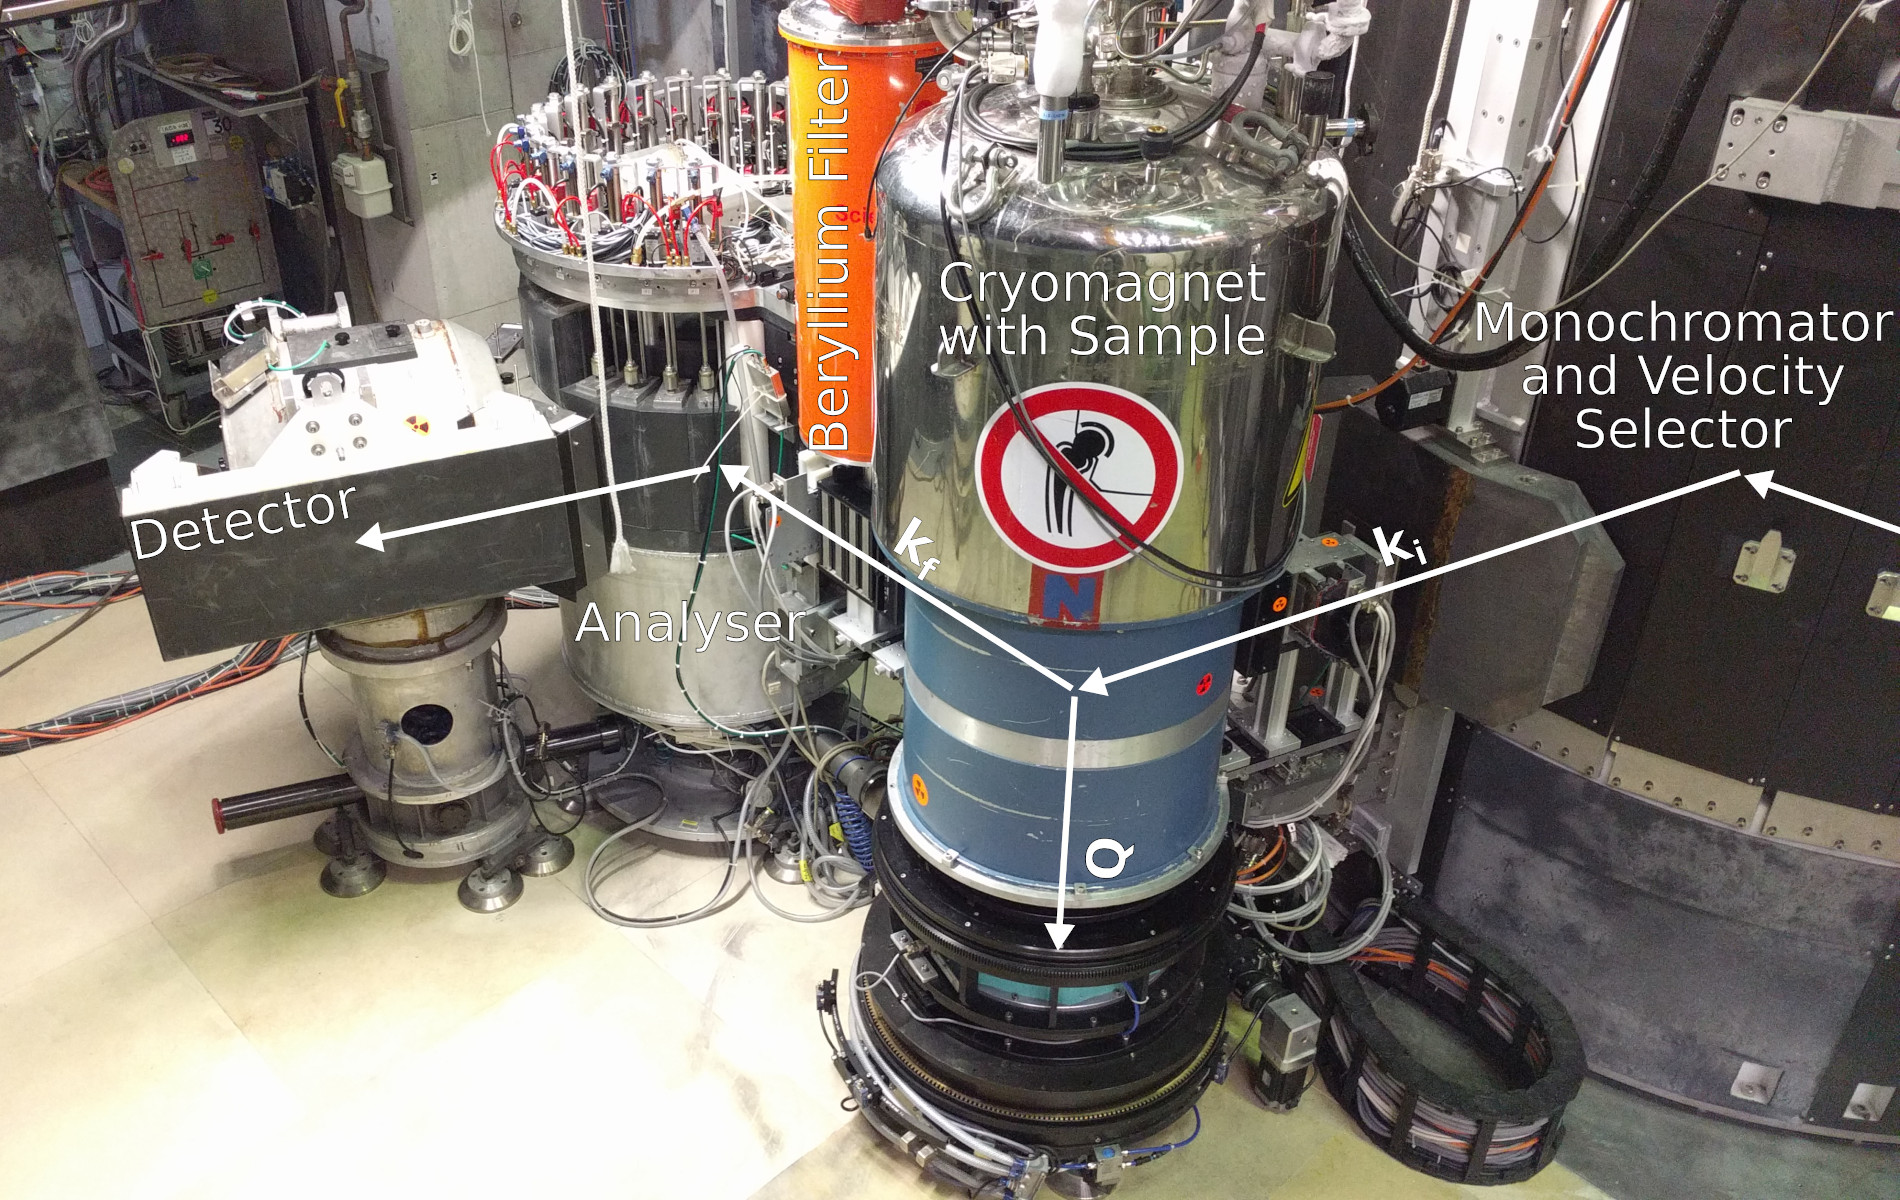
\includegraphics[width=0.66\textwidth]{figures/thales.jpg}
%	\end{centering}
%	\caption{The picture shows the triple-axis spectrometer \textit{ThALES} \cite{thales} at the ILL.}
%	\label{fig:tas}
%\end{figure}

%
% acknowledgements and thanks
% @author Tobias Weber <tweber@ill.fr>
% @date july-2021
% @license see 'LICENSE' file
%

\chapter*{Acknowledgements}
\addcontentsline{toc}{chapter}{Acknowledgements and Thanks}

I wish to thank my thesis advisors, Prof. Dr. Christian Icking and Dr. Lihong Ma, for accepting 
and supporting this project, for their advice and our regular discussions, the friendly atmosphere, 
as well as for always being available for questions.

Equal thanks to Dr. Martin B\"ohm, leader of the spectroscopy group at the ILL and instrument 
scientist at the Thales spectrometer, to Yannick Le Goc (computer scientist at the instrument 
control and electronics group), as well as Dr. Paul Steffens (Thales instrument scientist) for our 
regular discussions about various triple-axis automatisation projects, our experiments and the
instrumental aspects. I furthermore wish to thank Jérôme Locatelli (instrument control group) for
all the help with \textit{NOMAD}, the instrument control system at the ILL, and the technical discussions
about its internal details. 
Thanks to Dr. Paolo Mutti, the head of both the scientific computing and the instrument control group 
at the ILL, for supporting this project and for the great atmosphere and working environment there.

Also not to forget the continuing support from my former advisor for past theses, Prof. Dr. Peter B\"oni,
as well as from Prof. Dr. Christian Pfleiderer, Prof. Dr. Markus Garst, and Dr. Marc Janoschek in all our ongoing projects.

Financial support by the Institut Laue-Langevin via its \textit{P\^ole Formation} is gratefully acknowledged,
an I wish to thank Carole Fauchier for the administrative help.

Last but not least also many thanks to my family and to Soilhat for always being there for me!

%
% foreword
% @author Tobias Weber <tweber@ill.fr>
% @date sep-2021
% @license see 'LICENSE' file
%

\chapter*{Foreword}
\addcontentsline{toc}{chapter}{Foreword}
The present work is concerned about the development of a path-finding system for neutron triple-axis
spectrometers using the concepts of robot motion planning.
It touches upon multiple disciplines in physics and computer science. Among these are the field
of neutron scattering, concept of solid-state physics and crystallography for the physical part,
as well as Voronoi diagrams, graph theory and spatial index trees for robot motion 
planning, furthermore three-dimensional graphics and unit testing.
This work is organised in a manner to introduce important concepts with dedicated chapters that are
as self-contained as possible. These introductory chapters appear directly before the chapters that reference
them.

\paragraph{Layout of this work}
After some general introduction in chapter \ref{ch:intro}, the two subsequent chapters 
provide the necessary building blocks for the development of the path-finding algorithm that follows.
These are chapter \ref{ch:xtal}, which reviews important concepts from crystallography and
neutron scattering, namely crystal and instrument coordinate systems,
as well as chapter \ref{ch:algos}, which presents data structures and algorithms 
that are necessary for the path-finding.
Chapter \ref{ch:paths} is concerned about the general concept of path-finding and motion planning, providing
a review of different alternatives for the present problem as well as a high-level overview of the algorithm
to be developed in this work. The actual details and the implementation of the path-finding algorithm
is outlined in chapter \ref{ch:impl}.
Chapter \ref{ch:gl} contains a brief introduction to the mathematics of three-dimensional computer graphics.
This maths is made use of in chapter \ref{ch:gui} which is concerned about the user interfaces to the software
developed in this work. The user interfaces include a graphical one based on an interactive, three-dimensional
view of the instrument, as well as a purely command-line scripting interface.
Chapter \ref{ch:tests} describes unit testing necessary for maintaining
a reasonably sized software relatively bug-free.
The closing chapter, \ref{ch:outlook}, discusses the results and gives an outlook 
on future developments.

\paragraph{Accompanying software}
The source code of the software that is part of this work is provided on a supplementary 
medium together with compiled binary versions for several systems.
The source code is furthermore available via the DOI (digital object identifier) 
\href{https://doi.org/10.5281/zenodo.4625649}{10.5281/zenodo.4625649} and can be
accessed online via the URL \url{https://doi.org/10.5281/zenodo.4625649}.
An up-to-date list of possible future errata to this work will be provided under the DOI
\href{https://doi.org/10.5281/zenodo.5092159}{10.5281/zenodo.5092159} and the corresponding URL
\url{https://doi.org/10.5281/zenodo.5092159},
see appendix \ref{ch:online} for more details.


%\part{Main part}
%
% intro
% @author Tobias Weber <tweber@ill.fr>
% @date mar-2021
% @license see 'LICENSE' file
%

\chapter{Introduction}
\label{ch:intro}
In this first chapter, we introduce some basic concepts of neutron scattering and shortly present two types of
instruments typically found at research reactors (section \ref{sec:instruments}). A special emphasis is put
on triple-axis spectrometers (TAS) as the work-horse of inelastic neutron scattering. Finally, we summarise
the current state of autonomous experimentation (section \ref{sec:autonomous}).


\section{A brief history of neutron physics \label{sec:neutrons}}

The history of neutron physics begins in 1932 with the discovery of the neutron by James Chadwick, who used
alpha particles (helium nuclei) to bombard a beryllium-9 sample, thereby producing carbon-12 and one neutron
per reaction \cite[p. 1]{Jacrot2021}. The neutron that was created in this way was found to have a mass similar
to the proton ($m_n = 1.675\cdot10^{-27}\,\mathrm{kg}$, $m_p = 1.673\cdot10^{-27}\,\mathrm{kg}$), but, as the
name implies, no charge was detected \cite[p. 2]{Squires2012}. The absence of a charge makes the neutron very
useful for science, as it is subject to purely nuclear interactions with atomic nuclei, without any electrostatic
repulsion, for example by the electron hull \cite[p. 1]{Squires2012}.

In 1939, Otto Hahn used a Chadwick-type neutron source to irradiate uranium isotopes in an attempt to produce
heavy trans-uranium elements \cite{wiki_fission}. The measurements did not yield the expected results, because
instead of heavier elements, the experiment produced lighter elements. This was interpreted by Lise Meitner as
a splitting of the uranium nucleus, marking the discovery of nuclear fission \cite{wiki_fission}. A typical possible
channel of a fission reaction is the decay of uranium-235 into baryum-144 and krypton-89, where two to three
neutrons are produced by each reaction in addition to the daughter nuclei and energy \cite{wiki_fission}.

In 1942, Enrico Fermi made use of the excess neutrons that are obtained by each fission reaction to produce a
continuous, self-sustaining chain reaction in the first artificial nuclear reactor, the
\textit{Chicago Pile-1}~\cite[p.1]{Jacrot2021}.
It is interesting to note that while \textit{Chicago Pile-1} was the first \textit{artificial} nuclear reactor,
it was not the first one, strictly speaking. The first \textit{natural} reactor was discovered to have run more
than 1.5 billion years ago in Oklo, Gabun, at an average power of about 100 kW for a period of half a million
years \cite{wiki_oklo}.

The first research reactor, having a power of 3.5 MW~\footnote{As research reactors do not produce electricity,
the given numbers refer to thermal powers.} and being used for studies in solid-state physics, was built in
Oak Ridge, USA, in 1943, shortly after Fermi's pile \cite[p. 3]{Jacrot2021}.
Here, first neutron scattering experiments were performed by Clifford Shull using a two-axis diffractometer \cite[pp. 3, 37]{Jacrot2021}.

From there on, science advanced fast, and several centres dedicated to neutron research were founded around the world.
A selection of research reactors in operation today include the 20 MW \textit{Forschungsreaktor M\"unchen II}~\cite{web_mlz}
(FRM-II) at the Heinz-Maier-Leibnitz-Zentrum in Germany,
the 20 MW reactor at the NIST Center for Neutron Research~\cite{web_nist} (NCNR),
the 85 MW \textit{High Flux Isotope Reactor}~\cite{web_oakridge} (HFIR) at the Oak Ridge National Laboratory,
both based in the United States,
and the reactor of the Institut Laue-Langevin~\cite{web_ill} (ILL) in France, which - at 58 MW - is the most
powerful neutron source used for science in Europe.

Studying the structure and dynamics of crystals is made possible since neutrons emerging from the reactor can be
slowed down (moderated) into energy regions where their de Broglie wavelength $\lambda = h/p$ \cite[p. 89]{Gross2012}
corresponds to typical inter-atomic distances in crystal unit cells, which is of the order of 1 \AA{}ngstr\"om,
i.e. $10^{-10}$ m \cite[pp.1,3]{Squires2012}. In the formula, $p$ denotes the neutron momentum and $h$ Planck's constant.
Such a slowing-down of neutrons is usually performed using a secondary moderator outside the reactor's main moderator --
which itself sustains the nuclear fission -- for example using liquid $\mathrm{D_2O}$ \cite[p. 82]{Jacrot2021}.
Here, neutrons are brought into a new thermal equilibrium by elastic collisions with the nuclei of the moderator's
atoms \cite[p. 30]{Stacey2007}, i.e. the neutrons take the temperature and thus energy of the surrounding material.



\section{Instruments for neutron scattering \label{sec:instruments}}

While a modern research reactor houses a multitude of different instrument types, among them time-of-flight,
back-scattering and spin-echo spectrometers, furthermore Larmor, Laue and small-angle diffractometers, in
this section, we instead want to shortly present the most basic types of instrument, the two-axis diffractometer
and the triple-axis spectrometer. Together, the discovery of these two instruments by Clifford Shull and Bertram Brockhouse,
respectively, was awarded the 1994 Nobel Prize in Physics~\cite{web_nobel1994}.
A comprehensive introduction into these instruments, especially triple-axis spectroscopy, can be found in the
book by G. Shirane \cite{Shirane2002}. An advanced treatment of neutron scattering theory is given by
G. L. Squires \cite{Squires2012}.


\subsection{Two-axis diffractometers}

A two-axis diffractometer is used for determining the static structure of crystals, which are here typically provided
in powder form, but can also be single-crystals. It is the single most fundamental kind of machines in the field of
neutron scattering at research reactors. This instrument type consists of a single-crystal (meaning it comprises one
single grain), which is called ``monochromator'' and named after its function to pick out one specific wavelength,
$\lambda_i$, from the polychromatic neutron beam coming from the reactor core or from one of its moderators.
The physical principle behind wavelength selection is Bragg reflection \cite[p. 68]{Gross2012} \cite[p. 13]{Shirane2002},
\begin{equation}
	\label{eq:bragg}
	n \cdot \lambda_i \ =\  2 d \cdot \sin\left( \theta_M \right),
\end{equation}
with $\lambda_i$ being the neutron wavelength, $d$ the spacing of the crystal lattice planes from which scattering
takes place, $\theta_M$ half the monochromator scattering angle and $n$ the order of the reflection. A graphical
interpretation of Eq. \ref{eq:bragg} is depicted in Fig. \ref{fig:braggscattering}.

\begin{figure}[htb]
	\centering
	\includegraphics[width=0.35\textwidth]{figures/bragg.pdf}
	\caption[Bragg scattering.]{
		Bragg scattering on crystal planes having a spacing $d$. An incoming parallel neutron beam is reflected at an
		angle $2 \cdot \theta_M$ on both the upper and lower crystal plane, leading to a path difference of
		$2d \sin\theta$ between the beams. If the path difference is an integer multiple of the neutron wavelength,
		$\lambda_i$, the beams interfere constructively. Figure drawn after \cite[p. 68, Fig. 2.7]{Gross2012}. }
	\label{fig:braggscattering}
\end{figure}

The resulting monochromatic beam with the wavelength $\lambda_i$ and wavevector $\underline{k}_i$ is Bragg-scattered
a second time, this time from a sample powder containing small crystallites. Diffractometers typically contain hundreds
of neutron detectors surrounding the sample and picking up diffracted neutrons at a whole range of scattering angles
$2 \theta_S$. The scattering angles define the momentum transfer from the neutron to the sample as \cite[p. 11]{Shirane2002}
\begin{equation}
	\label{eq:Q}
	\hbar \underline{Q} \ =\  \hbar \left( \underline{k}_i - \underline{k}_f \right),
\end{equation}
where the two wavevectors $\underline{k}_i$ and $\underline{k}_f$ point along the propagation directions of the neutrons
before and after scattering from the sample, respectively. They both have the same magnitudes for diffraction, namely
$k_{i,f} = 2\pi / \lambda_i$ and are rotated by $2\theta_S$ from one another, see Fig. \ref{fig:diffraction} for a visualisation.
The symbol $\hbar$ denotes the reduced Planck's constant, $\hbar = h / \left( 2\pi \right)$.

\begin{figure}[htb]
	\centering
	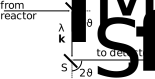
\includegraphics[width=0.35\textwidth]{figures/diffraction.pdf}
	\caption[Neutron diffraction.]{
		Principle of neutron diffraction. A polychromatic neutron beam coming from the reactor core is Bragg-scattered
		from the monochromator (M), picking out a single wavelength $\lambda_i$ and corresponding wavevector $\underline{k}_i$.
		The monochromatic beam is next scattered on the sample (S) at an angle $2\theta_S$, defining the direction of a
		wavevector $\underline{k}_f$. The momentum transferred from the neutron to the sample is given by Eq. \ref{eq:Q}
		as the difference of the two wavevectors.}
	\label{fig:diffraction}
\end{figure}

By the intensity of the sample's Bragg reflections, each of which appears at a different scattering angle $2\theta_S$
and thus momentum transfer $\hbar \underline{Q}$, the so-called static nuclear structure factor \cite[p. 25]{Shirane2002}
can be reconstructed. Absences of Bragg peaks determine the crystal symmetry given by its space group. Together,
they determine the structural build-up of the crystal.


\subsection{Triple-axis spectrometers}

In a two-axis diffractometer the scattering angle from a sample defines a momentum $\hbar \underline{Q}$ which is
transferred from the the neutron to the sample. It does not allow to select a sample-neutron energy transfer,
which is given by the de Broglie equation as \cite[p. 89]{Gross2012} \cite[p. 11]{Shirane2002}
\begin{equation}
	\label{eq:E}
	E \ =\ E_i - E_f \ =\ \frac{\left( \hbar k_i \right)^2}{2 m_n} - \frac{\left( \hbar k_f \right)^2}{2 m_n}.
\end{equation}
The constant $m_n$ is the neutron mass, for elastic scattering $k_i = k_f$.
The data obtained from such an instrument is instead integrated over all possible energy transfers.
This is no problem in practice, because elastic scattering, i.e. scattering with no energy transfer,
is usually many orders of magnitude stronger than inelastic scattering and any inelastic contribution
would not hide the elastic signals used for crystal structure determination.

Complementary to the two-axis instrument, a triple-axis spectrometer (TAS) is usually not used to study structures,
but instead measures the dynamics of the sample crystal. The samples used at TAS are usually in single-crystalline form.
At TAS machines, we are only interested in non-zero energy transfers, i.e. the cases when neutrons scattering from the
sample crystal excite collective modes. These modes typically comprise vibrations of the crystal's nuclei, called phonons,
which can be imagined as quantised sound waves \cite[pp. 123-137]{Shirane2002}. Another typical example includes the
coupled motions of the atom hull's electron spins, which are named spin-waves or magnons \cite[pp. 137-144]{Shirane2002}.

As the name implies, the difference of the TAS set-up compared to the two-axis diffractometer is one additional axis.
Having passed the sample, the neutrons may have changed their energy and thus wavelength and magnitude of the wavevector.
A further single-crystal is placed in the neutron path between the sample and the detector. Bragg scattering on this crystal
allows the detection of the neutron wavelength $\lambda_f$ after the sample, which remained unknown in the diffractometer.
Since we also know the incoming wavelength $\lambda_i$ before the scattering event at the sample, we can calculate the
transferred energy as given by Eq. \ref{eq:E}. This additional crystal and the corresponding instrument axis are named ``analyser''.
Fig. \ref{fig:spectroscopy} visualises the principles of the instrument, Fig. \ref{fig:thales} shows a typical triple-axis
instrument with its three axes, namely the monochromator in the right-hand side of the picture, the sample and the analyser
with the attached detector.

\begin{figure}[htb]
	\centering
	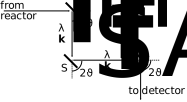
\includegraphics[width=0.4\textwidth]{figures/spectroscopy.pdf}
	\caption[Neutron spectroscopy.]{
		Principle of neutron spectroscopy. A polychromatic neutron beam coming from the reactor core is Bragg-scattered
		from the monochromator crystal (M), picking out a single wavelength $\lambda_i$ and wavevector $\underline{k}_i$.
		The monochromatic beam is next scattered on the sample (S) at an angle $2\theta_S$, defining a wavevector $\underline{k}_f$.
		The magnitude of $\underline{k}_f$ and thus $\lambda_f$ is determined by Bragg-scattering on the analyser crystal (A).
		The momentum and energy transfers are given by Eqs. \ref{eq:Q} and \ref{eq:E}, respectively. }
	\label{fig:spectroscopy}
\end{figure}

\begin{figure}[htb]
	\centering
	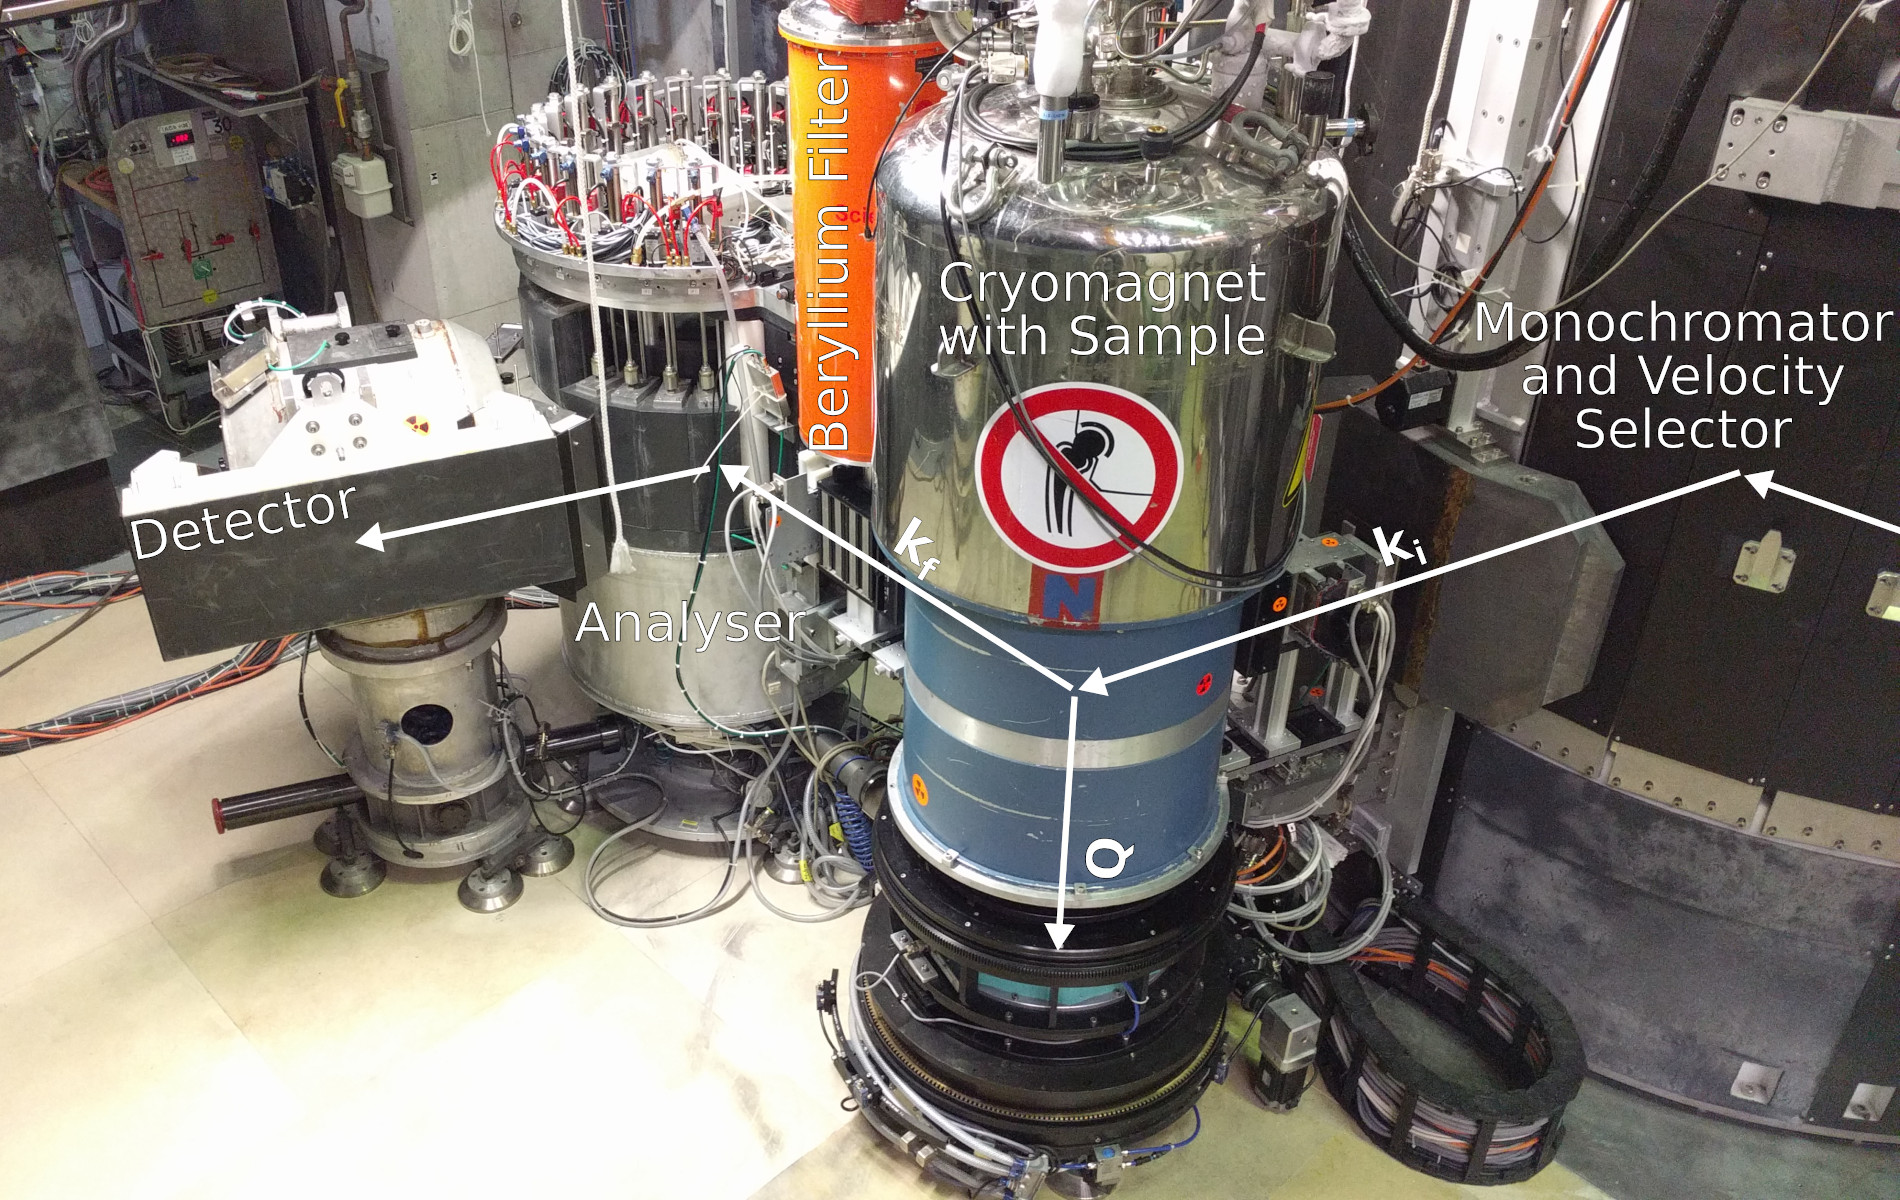
\includegraphics[width=0.75\textwidth]{figures/thales.jpg}
	\caption[The Thales instrument at the ILL.]{
		The triple-axis spectrometer ThALES \cite{thales} at the Institut Laue-Langevin in Grenoble, France. The neutron
		path from the reactor to the detector is marked as white arrows. The momentum transfer, $\hbar \underline{Q}$,
		is also shown. This picture is reproduced from the supplementary information of Ref. \cite{skxpaper}.}
	\label{fig:thales}
\end{figure}



\section{Autonomous experiments \label{sec:autonomous}}

Up until the end of 2019, TAS experiments usually required external scientists to stay at the research reactor for
typically one week and conduct the experiment together with the instrument's responsible scientists. Specifically
at the Institut Laue-Langevin (ILL), there had already been attempts \cite{Song2020} of the instrument control
and scientific computing groups to convince the instrument scientists of the benefits of instrumentation with full- or
semi-autonomous as well as remote control. Nevertheless, the impact had been limited.
Virtual experiments, on the other hand, had already been established in the simulation of actual experiments and in their
planning phase. Noteworthy software systems are \textit{McStas} \cite{McStas2020, McStas2021}, a neutron ray-tracing software based on the
Monte-Carlo method, simulating a large number of random neutrons and their interaction with various neutron-optical components,
as well as the software \textit{vTAS} \cite{vTAS2013}, which simulates the angles and crystal coordinates of a triple-axis
instrument and also provides support for calculating collisions with walls.

The situation changed significantly with the Covid-19 pandemic. Receiving visiting scientists from other countries had
not been possible anymore, or only to a very limited degree. Instead, remote experimentation and instrument control has
now become the new norm, with users connecting to a web interface from which the experiment can be planned and data can
be analysed~\cite{web_ill_visa}.
Discussions with instrument scientists take place via web-cams that have been installed at every instrument.

At the same time, the idea to automate manual tasks at instruments using algorithms and artificial intelligence has
gained significant traction, with first autonomous experiments being attempted at the ILL's spectroscopy group
\cite{web_ill_autonomous2020, Noack2021}.

As part of the current drive towards autonomous experimentation at the ILL, the goal of the present work is the design
and implementation of a software tool which enable an automatic path-finding for TAS instruments. Path-finding
is necessary for the instrument to circumvent obstacles in its way and for safe, collision-free movement close to walls.
Currently, this task has to be performed by the instrument scientists before each new scan series in a time-consuming fashion.
The current approach requires the instrument to be driven along the programmed scan path, but without measuring and with
the neutron beam from the reactor closed.
The scientist has to stay in the instrument space and watch the instrument as it moves to every scan position.
A manual stop has to be initiated when the instrument would collide with a wall, with itself, or when the rotation of one
of the axes would pull out a cable or tube.

An early attempt at automatic collision prevention and path-finding for a triple-axis spectrometer can be found in 
the 2006 work by M\"uhlbauer and Hradil \cite{Muehlbauer2006}, but their method is based on a simple grid search and thus
does not result in paths which keep the furthest distance to obstacles. A reason for such a solution might be
that computing power was not sufficient at that time to calculate the mesh of possible paths as it is 
done with the algorithms to be presented in the current work.



\section{Summary}

This chapter provided a short glance at neutron physics and the types of instrument typically used at research
reactors, with special emphasis on the triple-axis spectrometer. The complexity of the movement of these kind of
instruments necessitate the use of a path-finding system for a more effective set-up of measurements.
In the next chapter, we will introduce the coordinate systems used in crystallography and at TAS instruments,
and show how one set of coordinates transforms into the other.

%
% xtal formulas
% @author Tobias Weber <tweber@ill.fr>
% @date 13-jul-2018
% @license see 'LICENSE' file
%

\chapter{Crystal and Instrument Coordinate Systems}
\label{ch:xtal}

In this chapter we review the theory for conversion between crystal coordinates and scattering angles 
at the triple-axis instrument. Section \ref{sec:xtalcoords} introduces crystal coordinates and the so-called 
$UB$ matrix formalism, section \ref{sec:tasangles} calculates the corresponding TAS angles. 
The formalisms \cite{Lumsden2005} reviewed here are ubiquitous in neutron science, they are not only used 
in the control programs of triple-axis instruments, among them \textit{NOMAD} \cite{web_NOMAD} 
or \textit{NICOS} \cite{web_NICOS}, but are also employed in virtual instrument simulators like \textit{vTAS} \cite{vTAS2013} or 
\textit{McStas} \cite{McStas2020}, as well as in data analysis software like \textit{Mantid} \cite{Arnold2014}.

Note that this chapter has already been published in the manual of the software from Ref. \cite{Takin2021},
as well as in my (physics) PhD thesis \cite[pp. 139-143]{PhDWeber},
where the latter featured an earlier version of the same text, figures, and derivations.
Originally, these formulas were re-derived with the aid of the source
code of \textit{McStas'} \textit{templateTAS} virtual instrument \cite{web_mcstas_templateTAS, McStas2020}.


% ------------------------------------------------------------------------------------------------------------------------------------
\section{Fractional crystal coordinates \label{sec:xtalcoords}}

We begin by presenting the so-called $UB$ matrix formalism to convert between relative lattice units 
of a crystal and laboratory coordinates used in instrument space. This method has been described in 
Ref. \cite{Lumsden2005}. The derivation of the transformation matrices, $A$ and $B$, describing fractional
crystal coordinates, can be found in \cite{wiki_fractional}, which we follow here.

\subsection{$A$ and $B$ matrices}
\paragraph{Real-space crystal lattice}
The unit cell of the crystal is spanned by its three basis vectors $\left| a \right>$, $\left| b \right>$, and $\left| c \right>$, 
which -- in general -- are not perpendicular to one another, but instead enclose angles of $\alpha$, $\beta$, 
and $\gamma$, respectively, as shown in Fig. \ref{fig:cell}. 
To calculate the crystallographic $A$ matrix which transforms non-orthogonal crystal to orthogonal lab units, 
we first need to reduce the number of parameters.
The respective relations between the three basis vectors and their angles can be directly obtained via
their scalar products, where we follow the derivation in Ref. \cite{wiki_fractional}:

\vspace{\abovedisplayskip}
\begin{minipage}{0.317\textwidth}
	\begin{equation} \left< a | b \right > \ =\  ab \cos \gamma, \label{eq:ab} \end{equation}
\end{minipage}
\begin{minipage}{0.317\textwidth}
	\begin{equation} \left< a | c \right > \ =\  ac \cos \beta, \label{eq:ac} \end{equation}
\end{minipage}
\begin{minipage}{0.317\textwidth}
	\begin{equation} \left< b | c \right > \ =\  bc \cos \alpha. \label{eq:bc} \end{equation}
\end{minipage}
\vspace{\belowdisplayskip}

\begin{figure}
	\centering
	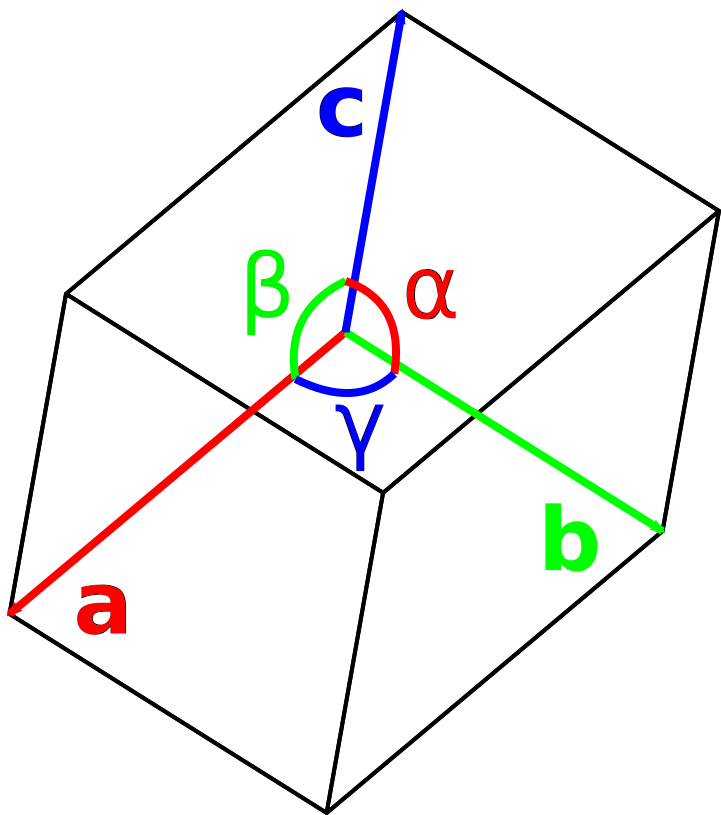
\includegraphics[width = 0.2 \textwidth]{figures/cell}
	\caption[Crystal unit cell.]{
		The unit cell of a crystal is given by its coordinate vectors $a$, $b$, and $c$ 
		as well as their angles $\alpha$, $\beta$, and $\gamma$.
		Figure drawn after the figure in Ref. \cite{wiki_fractional}.}
	\label{fig:cell}
\end{figure}


%\subsection*{Basis vectors}

The next goal is to explicitly write the components of the vectors $\left| a \right>$, $\left| b \right>$, and $\left| c \right>$ 
in terms of their lengths $a = \sqrt{\left< a | a \right>}$, $b = \sqrt{\left< b | b \right>}$, $c = \sqrt{\left< c | c \right>}$,
and the three angles.
To that end, we first choose -- without loss of generality -- $\left| a \right>$ along the $x$ axis, $\left| b \right>$ in the 
$xy$ plane, and $\left| c \right>$ in general:
\begin{equation} 
	\boxed{ \left| a \right> \ =\  \left( \begin{array}{c} a_1 = a \\ 0 \\ 0 \end{array} \right), }
	\hspace{0.5cm} \left| b \right> \ =\  \left( \begin{array}{c} b_1 \\ b_2 \\ 0 \end{array} \right),
	\hspace{0.5cm} \left| c \right> \ =\  \left( \begin{array}{c} c_1 \\ c_2 \\ c_3 \end{array} \right).
\end{equation}


Inserting $\left| a \right>$ and $\left| b \right>$ into Eq. \ref{eq:ab} gives the first component
of the $\left| b \right>$ vector:
\begin{equation} \left< a | b \right > \ =\  a_1 b_1 \ =\  ab \cos \gamma
\hspace{0.5cm} \Rightarrow \hspace{0.5cm} b_1 \ =\  b \cos \gamma. \end{equation}


Using the cross product between $\left| a \right>$ and $\left| b \right>$, we get the second component of $\left| b \right>$:
\begin{equation} 
	\left\Vert \left| a \right> \times \left| b \right> \right\Vert \ =\ 
	\left\Vert \left( \begin{array}{c} 0 \\ 0 \\ a_1 b_2 \end{array} \right) \right\Vert \ =\ 
	ab \sin \gamma \label{eq:crossab}
	\hspace{0.5cm} \Rightarrow \hspace{0.5cm} b_2 \ =\  b \sin \gamma.
\end{equation}

The vector $\left| b \right>$ is now complete:
\begin{equation} 
\boxed{ \left| b \right> \ =\  \left( \begin{array}{c} b \cos \gamma \\ b \sin \gamma \\ 0 \end{array} \right). } 
\label{eq:bvec} 
\end{equation}


Inserting $\left| a \right>$ and $\left| c \right>$ into Eq. \ref{eq:ac} gives the first component of $\left| c \right>$:
\begin{equation} \left< a | c \right > \ =\  a_1 c_1 \ =\  ac \cos \beta
\hspace{0.5cm} \Rightarrow \hspace{0.5cm} c_1 \ =\  c \cos \beta.
\end{equation}



Inserting $\left| b \right>$ and $\left| c \right>$ into Eq. \ref{eq:bc} yields the second component of $\left| c \right>$:
\begin{equation} \left< b | c \right > \ =\  b_1 c_1 + b_2 c_2 \ =\  bc \cos \alpha, \end{equation}
\begin{equation} b \cos \gamma \cdot c \cos \beta + b \sin \gamma \cdot c_2 \ =\  bc \cos \alpha
	\hspace{0.5cm} \Rightarrow \hspace{0.5cm}
	c_2 \ =\  \frac{c \cos \alpha - c \cos \gamma \cos \beta}{\sin \gamma}. \end{equation}



The last component, $c_3$, can be obtained from the vector length normalisation, $ \left< c | c \right> = c^2 $:
\begin{equation} \left< c | c \right > \ =\  c_1^2 + c_2^2 + c_3^2 \ =\  c^2, \end{equation}
\begin{equation} c_3^2 \ =\  c^2 - c_1^2 - c_2^2
	\hspace{0.5cm} \Rightarrow \hspace{0.5cm}
	c_3^2 \ =\  c^2 \left[1 - \cos^2 \beta - \left(\frac{\cos \alpha - \cos \gamma \cos \beta}{\sin \gamma} \right)^2 \right].
\end{equation}

The full vector $\left| c \right>$ is now reads:
\begin{equation} \boxed{ \left| c \right> \ =\  \left( \begin{array}{c}
	c \cdot \cos \beta \\
	c \cdot \frac{\cos \alpha - \cos \gamma \cos \beta}{\sin \gamma} \\
	c \cdot \sqrt{ \sin^2 \beta - \left(\frac{\cos \alpha - \cos \gamma \cos \beta}{\sin \gamma} \right)^2 }
\end{array} \right). } \end{equation}



The crystallographic $A$ matrix, which transforms real-space fractional to lab coordinates (\AA) \cite{Lumsden2005},
is formed with the basis vectors in its columns \cite[p. 631]{Arens2015}:
\begin{equation}
	A \ =\  \left(
		\begin{array}{ccc}
			\left| a \right> & \left| b \right> & \left| c \right>
		\end{array}
	\right).
\end{equation}
Explicitly written out using the basis vectors, the matrix reads \cite{wiki_fractional}:
\begin{equation}
	A \ =\  \left(
		\begin{array}{ccc}
			\begin{array}{c} a \\ 0 \\ 0 \end{array}
			& 
			\begin{array}{c} b \cos \gamma \\ b \sin \gamma \\ 0 \end{array} 
			& 
			\begin{array}{c}
				c \cdot \cos \beta \\
				c \cdot \frac{\cos \alpha - \cos \gamma \cos \beta}{\sin \gamma} \\
				c \cdot \sqrt{ \sin^2 \beta - \left(\frac{\cos \alpha - \cos \gamma \cos \beta}{\sin \gamma} \right)^2 }
			\end{array}
		\end{array}
	\right).
\end{equation}


\paragraph{Reciprocal-space crystal lattice}
For calculations in solid-state physics and neutron scattering, one does not normally use
the real-space crystal lattice, but instead thinks in term of the so-called reciprocal-space
lattice \cite[pp. 11-15]{Shirane2002}.
Reciprocal space is constructed in a way to facilitate calculations with momenta on a periodic lattice,
for that reason it is also sometimes called momentum or Fourier space.
A comparison of the same Bragg scattering in real vs. reciprocal space is shown in Fig. \ref{fig:braggscattering_recip}.
It is obvious that the reciprocal view greatly simplifies the image: Bragg scattering on what is a set of parallel
crystal planes in real space in panel (a) becomes a single point in reciprocal space \cite[p. 66]{Gross2012},
the so-called Bragg peak $\left| G \right>$ in panel (c). The reciprocal vector $\left| G \right>$ is
perpendicular to the original crystal planes and its length is related to their distance $d$ by
$\left\Vert G \right\Vert = 2\pi/d$ \cite[p. 66]{Gross2012}. Panel (c) also shows how the lattice vector
together with the neutron beam directions forms the so-called scattering triangle, which is 
ubiquitous in visualisations of neutron scattering geometry \cite[pp. 14-15]{Shirane2002} and which will be 
discussed in the next section.
\begin{figure}[htb]
	\centering
	\includegraphics[width=1\textwidth]{figures/bragg_recip}
	\caption[Real and reciprocal lattice scattering.]{
		(a) Bragg scattering on crystal planes having a spacing $d$, viewed from real space.
			Figure drawn after Ref. \cite[p. 68, Fig. 2.7]{Gross2012}.
		(b) A view mixing real and reciprocal space. The reciprocal lattice vector, $\underline{G}$,
			is perpendicular to the real space crystal planes.
		(c) Bragg scattering viewed from reciprocal space. The direction of the incoming and outgoing
			neutron beams define wavevectors $\underline{k}_i$ and $\underline{k}_f$.
			Such a representation is called a scattering diagram or scattering triangle
			\cite[p. 14, Fig. 1.5]{Shirane2002}.}
	\label{fig:braggscattering_recip}
\end{figure}

From the construction of reciprocal space, it can be shown that the basis vectors of reciprocal space
are mutually perpendicular to the corresponding real space basis vectors \cite[p. 60]{Gross2012}.
This directly leads to the so-called $B$ matrix, which transforms reciprocal-space relative lattice units (rlu)
to lab coordinates (1/\AA) \cite{Lumsden2005}, is \cite[p. 60]{Gross2012}:
\begin{equation} B \ =\  2 \pi A^{-t}, \end{equation}
where $-t$ denotes the transposed inverse.
We can now also determine the metric tensor \cite[pp. 807-809]{Arens2015} corresponding to the coordinate
system defined by the $B$ transformation matrix, it reads \cite[p. 808]{Arens2015}:
\begin{equation}
	\left(g_{ij}\right) \ =\  \left<\underline{b}_i | \underline{b}_j \right> \ =\  B^T B,
\end{equation}
where the reciprocal basis vectors $\left| \underline{b}_i \right>$ form the columns of $B$ \cite[p. 631]{Arens2015}.

A rigorous introduction into the reciprocal crystal lattice can be found in the book by Gross
and Marx \cite[pp. 58 - 67]{Gross2012}.


\subsection{Example: lengths and angles in the reciprocal lattice}
Having a metric makes it straightforward to calculate lengths and angles.
The length of a reciprocal lattice vector $\left| G \right>$ seen from the lab system is 
(in 1/\AA{} units) \cite[p. 808]{Arens2015}:
\begin{equation}
	G  \ =\ 
	\left\Vert \left< G | G \right> \right\Vert \ =\  \sqrt{\left< G | G \right>}
		\ =\  \sqrt{G_i G^i} \ =\  \sqrt{g_{ij} G^i G^j}.
\end{equation}
The angle $\theta$ between two Bragg peaks $\left| G \right>$ and $\left| H \right>$ 
is given by their dot product \cite[p. 808]{Arens2015}:
\begin{equation}
	\frac{\left< G | H \right>}{\left\Vert \left< G | G \right> \right\Vert
		\cdot \left\Vert \left< H | H \right> \right\Vert} \ =\
	\frac{g_{ij} G^i H^j }{\sqrt{g_{ij} G^i G^j} \sqrt{g_{ij} H^i H^j}} \ =\  \cos \theta.
\end{equation}

Please note that if an index appears twice, both as subscript as well as a superscript, 
a summation over it is implied, see Ref. \cite{wiki_summation}.


\subsection{$U$ matrix}
The $B$ matrix alone yields the transformation from the non-orthogonal and reciprocal crystal 
coordinate system into the orthogonal lab units \cite{Lumsden2005}.
However, it does not yet take into account the actual rotation of the crystal so that a specific plane, 
the so-called scattering plane, can be accessed by the two-dimensional movements of the instrument. 
Such a rotation is performed by the $U$ matrix, whose rows contain two vectors inside the desired 
scattering plane and the plane normal \cite{Lumsden2005}.
These basis vectors are usually chosen along two orientation Bragg reflections \cite[pp. 87-88]{Shirane2002}
and are expressed in the orthogonal lab system, i.e. they are pre-multiplied by $B$.
For $U$ to be a rotation matrix, the basis vectors are normalised using, for instance, the
Gram-Schmidt algorithm \cite[p. 744]{Arens2015} \cite[pp. 269-270]{Arfken2013} or 
QR decomposition \cite[pp. 269-272]{Scarpino2011}.

In summary, a coordinate point $\left|Q_{\mathrm{rlu}}\right>$, which is given in relative lattice 
units of the reciprocal crystal, 
is transformed by the $B$ matrix into the orthogonal lab units used at the instrument \cite{Lumsden2005}.
It is then rotated by the $U$ matrix to account for the actual crystal orientation \cite{Lumsden2005}:
\begin{equation}
	\left|Q_{\mathrm{lab}}\right> \ =\  U \cdot B \cdot \left|Q_{\mathrm{rlu}}\right>.
	\label{eq:UBtrafo}
\end{equation}
In the rest of this work we will not use the $U$ matrix explicitly, though, but instead directly work 
with its basis vectors and the metric tensor. This is just a formality, though, the mathematics are the same.

% ------------------------------------------------------------------------------------------------------------------------------------




% ------------------------------------------------------------------------------------------------------------------------------------
\section{Scattering triangle and TAS angles \label{sec:tasangles}}

With the metric tensor \cite[pp. 807-809]{Arens2015} of the crystal coordinate system, we can now calculate the scattering angles
$2 \theta_M$, $2 \theta_S$, and $2 \theta_A$ from the monochromator, sample and analyser, respectively. 
The derivation of basic scattering geometries in triple-axis spectrometers can be found in \cite[Ch. 1.3]{Shirane2002},
which we follow here. 
The explicit calculation of the TAS angles based on the $UB$ formalism was originally presented in Ref. \cite{Lumsden2005}.

For the monochromator and analyser, the crystal angles $\theta_M$ and $\theta_A$ are coupled to 
their scattering angles, they are simply half their value, because the Bragg condition of Eq. \ref{eq:bragg}
always has to be fulfilled.
The crystal rotation for the sample is not necessarily half its scattering angle, $\Theta_S \ne 2\theta_S/2$, 
though, because the instrument can be freely positioned at any point of reciprocal crystal space.

The monochromator and analyser scattering angles follow directly from Bragg's equation 
\cite[p. 68]{Gross2012} \cite[p. 13]{Shirane2002}:

\begin{minipage}{0.45\textwidth}
	\centering
	\begin{equation} 2 d_{M}\sin \theta_{M} \ =\  n \lambda_{i}, \end{equation}
	\begin{equation} 2 k_{i} \sin \theta_{M} \ =\  2 \pi n / d_{M}, \end{equation}
	\begin{equation} \boxed{ \theta_{M} \ =\  \arcsin \left( \frac{\pi n}{d_{M} \cdot k_{i}} \right). } \end{equation}
\end{minipage}
\begin{minipage}{0.45\textwidth}
	\centering
	\begin{equation} 2 d_{A}\sin \theta_{A} \ =\  n \lambda_{f}, \end{equation}
	\begin{equation} 2 k_{f} \sin \theta_{A} \ =\  2 \pi n / d_{A}, \end{equation}
	\begin{equation} \boxed{ \theta_{A} \ =\  \arcsin \left( \frac{\pi n}{d_{A} \cdot k_{f}} \right). } \end{equation}
\end{minipage}

%\vspace{0.5cm}

To determine the sample scattering angle $2 \theta_S$, we use the so-called scattering triangle, see 
Fig. \ref{fig:scattering_triangle}, whose connection to the neutron beam direction has already 
been established in the previous section.
The scattering triangle can be directly determined by the angles the instrument is positioned at \cite[pp. 14-15]{Shirane2002}: 
For that, we have a look at the incoming and final neutron wavevectors $\left| k_i \right>$ and $\left| k_f \right>$, 
whose directions (but not lengths!) correspond directly to the neutron paths before and after the sample, 
respectively, as shown on the left-hand side of Fig. \ref{fig:scattering_triangle}. We can rearrange them so 
that their tips meet, as depicted on the right-hand side of Fig. \ref{fig:scattering_triangle}, where the 
scattering triangle is formed by $\left| k_i \right>$ and $\left| k_f \right>$ together with the
scattering vector $\left| Q \right> = \left| k_i \right> - \left| k_f \right>$ \cite[p. 14]{Shirane2002}.
Here, the two wavevectors enclose the scattering angle $2 \theta_S$.

\begin{figure}
	\begin{center}
		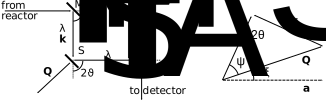
\includegraphics[width = 0.75 \textwidth]{figures/tas_triangle}
	\end{center}
	\caption[TAS layout and scattering triangle.]{
		Triple-axis layout (left) and corresponding scattering triangle (right).
		Figures inspired by Ref. \cite[p. 72, Fig. 3.8]{Shirane2002} and \cite[p. 15, Fig. 1.6]{Shirane2002}, respectively.
		\label{fig:scattering_triangle}}
\end{figure}

We can calculate $2 \theta_S$ via the cosine theorem \cite[pp. 694-695]{Arens2015}, i.e.
by forming the scalar product of $\left| Q \right>$ with itself in lab units \cite[p. 11]{Shirane2002}:
\begin{equation} 
	\left| Q \right> \ =\  \left| k_i \right> - \left| k_f \right>,
\end{equation}
\begin{equation} 
	\left< Q | Q \right> \ =\  \left( \left< k_i \right| - \left< k_f \right| \right) \cdot \left( \left| k_i \right> - \left| k_f \right> \right)
	\ =\  \left< k_i | k_i \right> + \left< k_f | k_f \right> - 2 \left< k_i | k_f \right>,
\end{equation}
\begin{equation} 
	Q^2 \ =\  k_i^2 + k_f^2 - 2 k_i k_f \cos \left( 2 \theta_S \right),
\end{equation}
\begin{equation}
	\boxed{ 2 \theta_S \ =\  \sigma_s \cdot \arccos \left( \frac{k_i^2 + k_f^2 - Q^2}{2 k_i k_f} \right). }
\end{equation}

We could now -- as is done in the work by Lumsden \textit{et al.} \cite{Lumsden2005} -- calculate the length
$Q$ of the vector $\left| Q \right>$ by explicitly transforming it into lab units using Eq. \ref{eq:UBtrafo}.
Instead, we directly determine its length in lab units from its native rlu system using the covariant dot 
product \cite[p. 808]{Arens2015}:
\begin{equation}
	Q %\ =\ Q_{\mathrm{lab}} 
	\ =\ 
	\sqrt{Q^{\mathrm{rlu}}_i Q_{\mathrm{rlu}}^i} \ =\  \sqrt{g_{ij} Q_{\mathrm{rlu}}^i Q_{\mathrm{rlu}}^j}.
\end{equation}

As we could scatter in either clockwise or counter-clockwise direction, $2 \theta_S$ can be positive or negative.
The sign of $2 \theta_S$ is given by the sample scattering sense $\sigma_s = \pm 1$.


%\vspace{0.5cm}


The final and most complicated angle to determine is the sample rotation $\Theta_S$.
It is given by the angle of the incoming wavevector $\left| k_i \right>$ to an (arbitrary) direction 
$\left| a \right>$ which is known from sample orientation, this is usually a Bragg peak \cite[p. 87]{Shirane2002}.
If we were to explicitly use the $U$ matrix here, this vector would be one of its rows.
The situation is shown in the right panel of Fig. \ref{fig:scattering_triangle}.
We split $\Theta_S$ into the angle $\psi$ between $\left| k_i \right>$ and $\left| Q \right>$ 
and the angle $\xi$ between $\left| Q \right>$ and $\left| a \right>$:
\begin{equation} \boxed{ \Theta_S \ =\  180^{\circ} - \left( \psi + \xi \right).} \end{equation}


%\vspace{0.5cm}


The angle $\psi$ between $\left| k_i \right>$ and $\left| Q \right>$ is determined from the scattering triangle, as before
in lab units:
\begin{equation}
	\left| k_f \right> \ =\  \left| k_i \right> - \left| Q \right>,
\end{equation}
\begin{equation} 
	\left< k_f | k_f \right> \ =\  \left( \left< k_i \right| - \left< Q \right| \right) \cdot \left( \left| k_i \right> - \left| Q \right> \right)
	\ =\  \left< k_i | k_i \right> + \left< Q | Q \right> - 2 \left< k_i | Q \right>,
\end{equation}
\begin{equation}
	k_f^2 \ =\  k_i^2 + Q^2 - 2 k_i Q \cos \psi,
\end{equation}
\begin{equation}
	\boxed{ \psi \ =\  \sigma_s \cdot \arccos \left( \frac{k_i^2 + Q^2 - k_f^2}{2 k_i Q} \right).}
\end{equation}


%\vspace{0.5cm}


The angle $\xi$ between $\left| Q \right>$ and orientation vector $\left| a \right>$ is also determined 
from the properties of the scalar product.
Here we have to use its covariant form via the metric tensor, $g_{ij}$, \cite[p. 808]{Arens2015},
because $\left| a \right>$ is a coordinate in crystal space naming a Bragg reflection,
while $\left| Q \right>$ would natively live, as before, in instrument space, where we can thus avoid transforming to,
unlike Ref. \cite{Lumsden2005}.
\begin{equation} 
	\boxed{ \xi \ =\  
\sigma_{\mathrm{side}} \cdot \arccos \left( \frac{ \left< Q_{\mathrm{rlu}} | a \right> }{ \sqrt{\left< Q_{\mathrm{rlu}} | Q_{\mathrm{rlu}} \right>} \sqrt{\left< a | a \right>} } \right) \ =\  
\sigma_{\mathrm{side}} \cdot \arccos \left( \frac{ Q_{\mathrm{rlu}}^i g_{ij} a^j }{ \sqrt{Q_{\mathrm{rlu}}^i g_{ij} Q_{\mathrm{rlu}}^j} \sqrt{a^i g_{ij} a^j} } \right).}
\label{eq:xi}
\end{equation}

The sign, $\sigma_{\mathrm{side}}$, of $\xi$ depends on which side of the orientation vector 
$\left| a \right>$ the scattering vector $\left| Q_{\mathrm{rlu}} \right>$ is located. 
The sign can be found by calculating the (covariant) cross product of $\left| a \right>$ and 
$\left| Q_{\mathrm{rlu}} \right>$ to give an out-of-plane vector $\left| x \right>$ which can be compared with 
the given scattering plane up vector.
The covariant cross-product is calculated as \cite[p. 815]{Arens2015}:
\begin{equation}
	x^l \ =\  g^{li} \epsilon_{ijk} a^j Q_{\mathrm{rlu}}^k,
\end{equation}
where $\epsilon_{ijk}$ is the general Levi-Civita symbol formed from the determinant of the 
basis vectors $\left| \underline{b}_i \right>$, see Ref. \cite[p. 815]{Arens2015}:
\begin{equation}
	\epsilon_{ijk} \ =\  \left|
		\begin{array}{ccc} \left| 
			\underline{b}_i \right> & \left| \underline{b}_j \right> & \left| \underline{b}_k \right>
		\end{array} \right|.
\end{equation}



\paragraph*{Special case}
For cubic crystals with $\alpha = \beta = \gamma = 90^{\circ}$ and the lattice constants all equal, 
$a = b = c$, the metric tensor is diagonal, $g_{ij} = \delta_{ij} \cdot \left( 2\pi / a \right)^2$.
With that Eq. \ref{eq:xi} simplifies to:
\begin{equation}
	\xi \ =\  \sigma_{\mathrm{side}} \cdot \arccos \left( \frac{ Q^{\mathrm{rlu}}_i a^i }{ \sqrt{Q^{\mathrm{rlu}}_i Q_{\mathrm{rlu}}^i} \sqrt{a_i a^i} } \right).
\end{equation}
% ------------------------------------------------------------------------------------------------------------------------------------


\section{Summary}
This chapter introduced some important concepts from solid-state physics and crystallography that are essential
for an understanding of the basic coordinate system transformations from the generally non-orthogonal (real or 
reciprocal) crystal coordinates to the orthonormal lab coordinates used at the instrument.
In practice, it is the crystal coordinates that are entered into the instrument control software by
the user, not the raw instrument angles. A pathfinding system for triple-axis spectrometers thus has to know both.
Internally, it will be more convenient for the software to use instrument-related coordinates, as we will see in 
the following chapters, but the input and output will be in crystal coordinates.

Having established all the necessary physical foundations, the next chapter will proceed to do the same for the 
essential concepts in computer science before putting everything together in a pathfinding algorithm.

%
% algorithms
% @author Tobias Weber <tweber@ill.fr>
% @date aug-2021
% @license see 'LICENSE' file
%

\chapter{Basic Concepts, Algorithms and Data Structures}
\label{ch:algos}
The  path-finding algorithm and implementation that will be presented in the following chapters
employ several different concepts, data structures and methods.
Among these concepts are the Voronoi diagram (section \ref{sec:voro}),
graph data structures and algorithms on them (section \ref{sec:graphs}),
as well as spatial index trees (section \ref{sec:indextrees}).
In this chapter, these basic building blocks are reviewed in a general manner.



\section{Voronoi diagrams}
\label{sec:voro}
As we will see in the next chapter, a concept that will play a central role for the path-finding 
algorithm of this work is the Voronoi diagram.
A good review of Voronoi diagrams is given in Ref. \cite[Ch. 7, pp. 147-171]{Berg2008} 
and in \cite[Ch. 5, pp. 209f]{FUH_geo2020}, which we follow in this chapter.

Starting with some basic definitions, a \textit{Voronoi diagram} is a set of 
\textit{bisectors}, $B\left(\underline{x},\, \underline{y}\right)$, separating \textit{Voronoi regions}.
A Voronoi region names the set of points $\underline{x}$ in a vector space $V$ that are closest to 
a given site $\underline{s}$ under a given metric $\left\Vert \cdot \right\Vert$, which measures distances in $V$.
The site can either be isolated vertices, lines or any other finite object.
Formally, the bisector between two sites $\underline{s}_1$ and $\underline{s}_2$ is, 
generalising from \cite[p. 140]{Icking2001},
\begin{equation}
	B\left(\underline{s}_1,\, \underline{s}_2\right)\ =\ \left\{ \underline{x} \in V \ |\ 
		\left\Vert \underline{x} - \underline{s}_1 \right\Vert = \left\Vert \underline{x} - \underline{s}_2 \right\Vert \right\}.
	\label{eq:bisector}
\end{equation}
Even though this definition of Voronoi diagrams does not restrict the vector space to the $\mathbb{R}^n$ 
and the underlying metric to the usual Euclidian one, 
\begin{equation}
	\left\Vert \underline{x} \right\Vert_2 \ =\ \sqrt{\left<x | x \right>},
\end{equation}
they are nevertheless implied in the rest of this work if nothing else is specified.
Specifically, we thus set $V = \mathbb{R}^2$ and $\left\Vert \cdot \right\Vert = \left\Vert \cdot \right\Vert_2$. 
Please refer to Ref. \cite{Icking2001} for other metrics and to Ref. \cite{Boissonnat2006} for further 
generalisations of the concept of Voronoi diagrams.



\subsection{Voronoi diagrams for vertex sites}
The simplest case to consider is the Voronoi diagram where the sites are vertices, 
the vector space is the $\mathbb{R}^n$ and the metric Euclidian. This case is called the 
\textit{affine Voronoi diagram} in the work by Boissonnat \textit{et al.},
its bisectors consist of $n-1$-dimensional hyperplanes \cite[pp. 72-81]{Boissonnat2006}.
Specifically for $\mathbb{R}^2$, the bisectors are either line segments or infinite lines, 
depending on the open or closed nature of the corresponding Voronoi region.
An example of two or several vertex sites and their bisectors is shown in Fig. \ref{fig:vertex_voro}.

\begin{figure}[htb]
	\begin{minipage}{1 \textwidth}
		\begin{center}
			\includegraphics[width = 0.35 \textwidth]{figures/vertex_voro}
		\end{center}
		\vspace{0.5cm}
		\begin{center}
			\includegraphics[width = 0.7 \textwidth]{figures/vertex_voro2}
		\end{center}
	\end{minipage}
	\caption[Voronoi diagrams for vertices.]{
		Top panel: Voronoi diagram for two vertex sites, $s_1$ and $s_2$. 
			The bisector, $B\left(s_1, s_2\right)$, separates $\mathbb{R}^2$ 
			into two open Voronoi regions forming half-planes.
		Bottom panel: Voronoi diagram for ten vertex sites, $s_1,\, s_2,\, ...,\, s_{10}$.
		The black lines are the bisectors of the Voronoi regions, where the solid lines are of finite size
		and delimit closed Voronoi regions. The dashed lines are of infinite length and delimit open Voronoi regions.
		The figure has been calculated using the test program that will be described in chapter \ref{sec:tests_hull}.
		\label{fig:vertex_voro}}
\end{figure}


\paragraph{Physical application: Brillouin zones}
Vertex-site Voronoi diagrams are ubiquitous in solid-state physics and all its connected disciplines
like neutron scattering, magnetism, etc., although they are not called so in these fields.
In physics, one usually thinks in terms of the reciprocal (dual, Fourier) space of a crystal lattice, as discussed
in chapter \ref{ch:xtal}. Due to the periodic nature of the crystal and its reciprocal space, one can define a smallest
cell around the vertex sites in reciprocal space (here called ``Bragg peaks'', as discussed before) for which all physics is 
the same, the so-called \textit{first Brillouin zone} of the reciprocal lattice \cite[pp. 63-64]{Gross2012}. 
The definition of the first Brillouin zone corresponds to that of the Voronoi region of the Bragg peaks.
The crystal and its reciprocal lattice are assumed to be infinite. This is a good approximation as one usually
considers physics in the \AA{}ngstr\"om scale ($10^{-10}\,\mathrm{m}$), while the crystals used in neutron scattering usually have volumes on the
$cm^3$ scale. Having an infinite lattice has the effect that the Voronoi diagram does not possess any open regions.
As the crystal is regular and periodic, only one shape of Voronoi region exists, which repeats to fill the
entire reciprocal space without gaps.
Typical examples of Brillouin zone shapes for cubic crystals and two-dimensional cuts through them 
are shown in Fig. \ref{fig:cubic_bzs}.

\begin{figure}[h]
	\begin{center}
		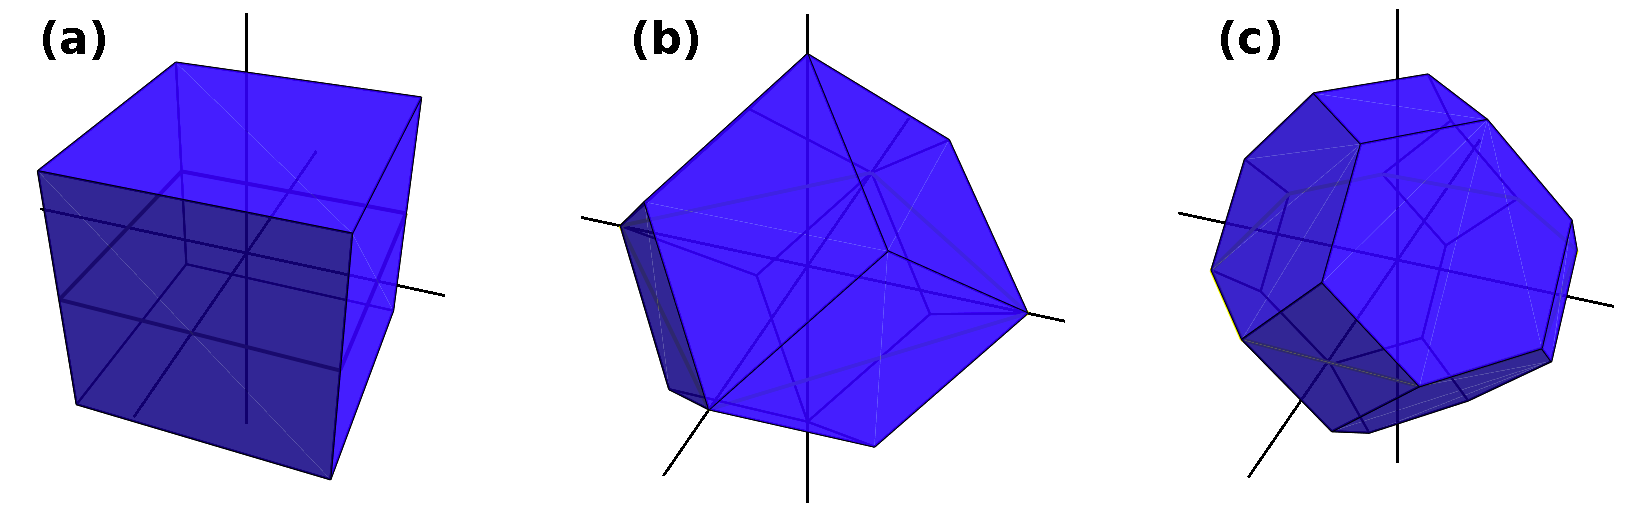
\includegraphics[width = 0.95 \textwidth]{figures/bz}

		\vspace{0.5cm}
		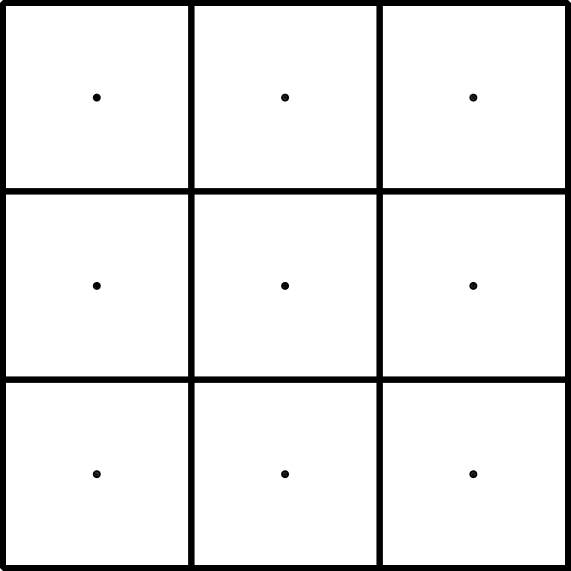
\includegraphics[width = 0.2 \textwidth]{figures/sc}
		\hspace{2.2cm}
		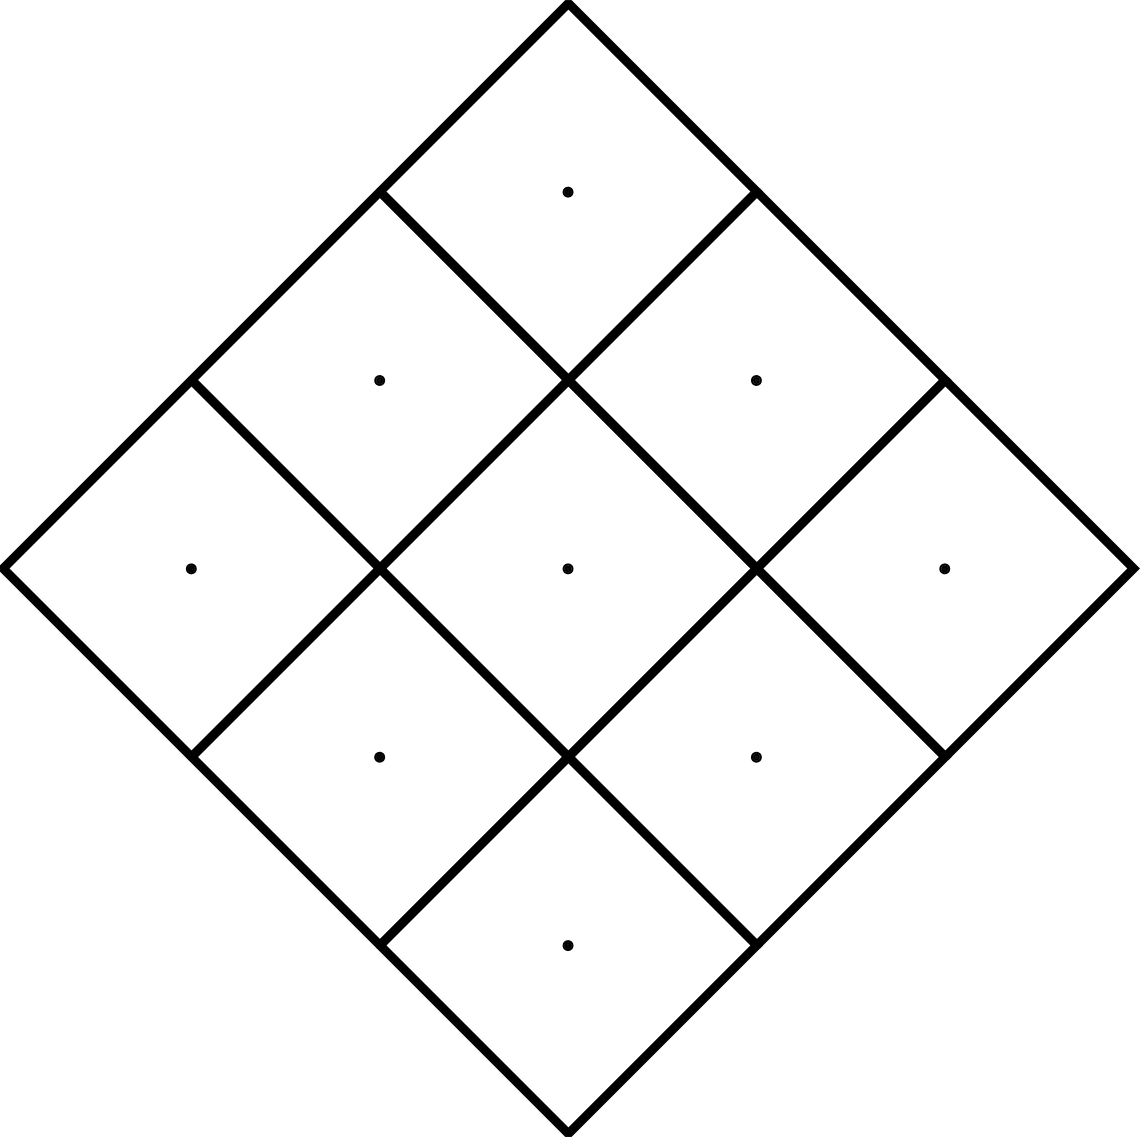
\includegraphics[width = 0.2 \textwidth]{figures/bcc}
		\hspace{2.2cm}
		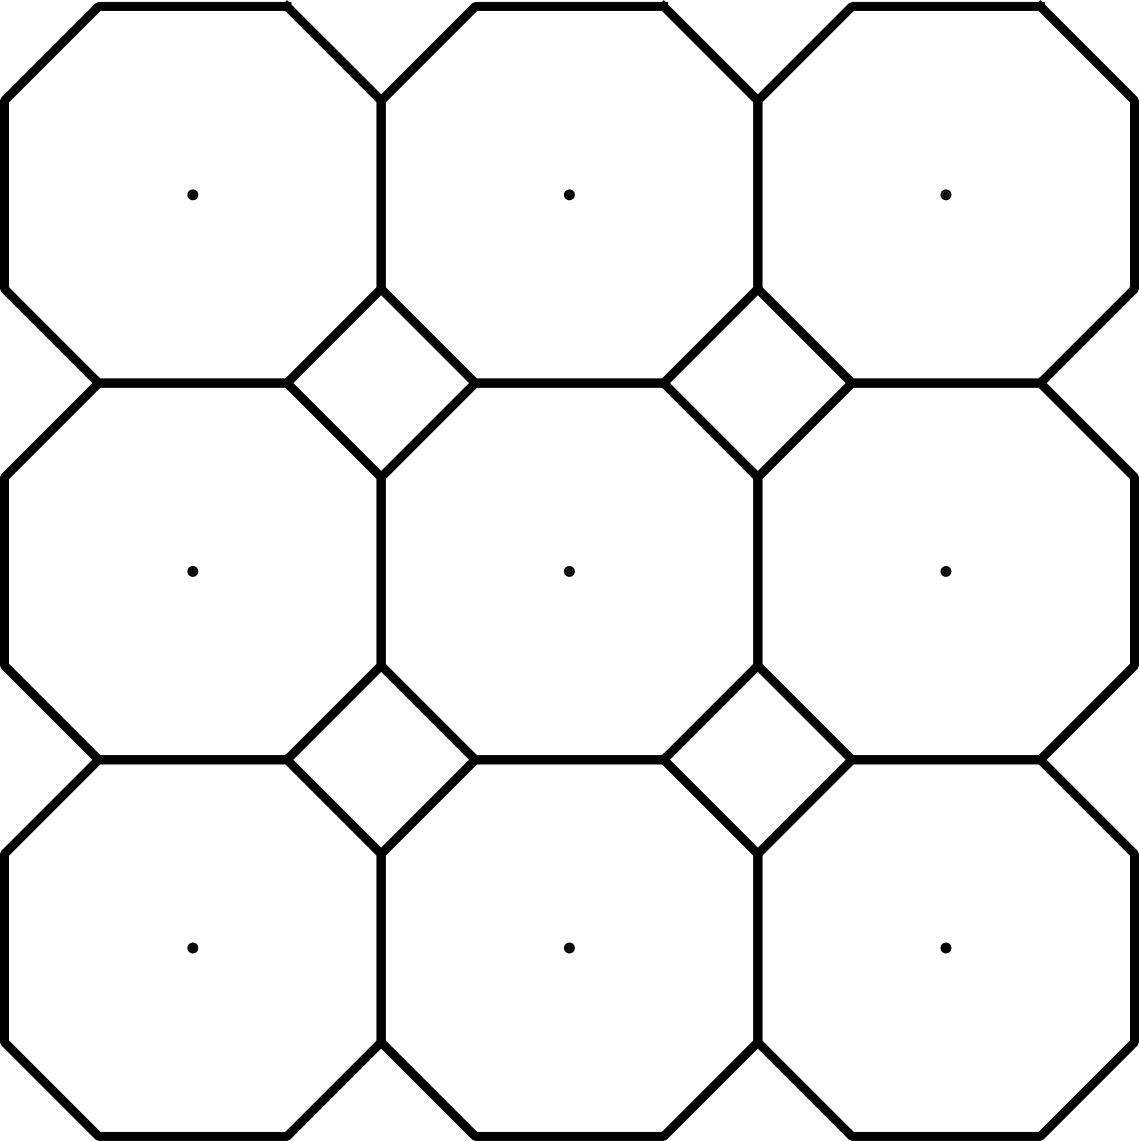
\includegraphics[width = 0.2 \textwidth]{figures/fcc}
	\end{center}
	\caption[Brillouin zones.]{
		First Brillouin zone for
			(a) a simple cubic,
			(b) a body-centred cubic, and
			(c) a face-centred cubic crystal lattice.
		In the top panels, 3-d views of only the bisectors are shown.
		In the bottom panels, 2-d cuts through the horizontal plane show the Brillouin zones 
		completely filling the space. The vertex sites (Bragg peaks) are shown as small dots.
		Such 2-d views are typically used for experiments at triple-axis spectrometers.
		The apparent gaps in in the 2-d cut of panel (c) come from Brillouin zones which are 
		above or below the cutting plane.
		Calculated using the \textit{Takin} software \cite{Takin2021, Takin2017, Takin2016}.
		\label{fig:cubic_bzs}}
\end{figure}



\subsection{Voronoi diagrams for line segment sites}
\label{sec:voro_ls}
Voronoi diagrams over the vector space $\mathbb{R}^n$ with either a non-Euclidian metric or sites that
are not point-shaped are called non-affine and possess curved bisectors \cite[p. 72]{Boissonnat2006}.
We now look at the special case of Voronoi diagrams over the $\mathbb{R}^2$ constructed from line segments.
A description of this case can be found in \cite[Ch. 7.3, pp. 160-163]{Berg2008} and in 
\cite[pp. 242-247]{FUH_geo2020}, whose descriptions we follow in this section.

For this case, the Voronoi region of a line $l_i$ consists of all points in $\mathbb{R}^2$ that 
are closest to $l_i$. The bisector is the boundary between the Voronoi regions of two line segments 
$l_i$ and $l_j$, $i \neq j$,
and is the curve of equal distance between the two line segments $l_i$ and $l_j$.
Its shape is either linear or quadratic, where, in the linear case, the bisector curve can also be either
finite or infinite \cite[pp. 243-244]{FUH_geo2020}.

A linear bisector is obtained for the distance calculated between two line segment endpoints or between two inner 
points on the line segments which are not the endpoints.
This can easily be seen, because, (a) in the case of two endpoints, the middle perpendicular line between these 
two points is equidistant to them; and (b) in the case of two line segments, the angular bisector of the two lines is
equidistant to them \cite[pp. 243-244]{FUH_geo2020}.
On the other hand, the bisector curve segment follows a parabolic shape if the distance is calculated 
between a line segment endpoint and one inner point of the other segment. This is the same as the bisector between
a point and a line and its parabolic shape is proven in \cite[pp. 260-261]{FUH_geo2020}.
An example of two or several line segment sites and their bisectors is shown in Fig. \ref{fig:linesegs_voro}.

\begin{figure}[htb]
	\begin{minipage}{1 \textwidth}
		\begin{center}
			\includegraphics[width = 0.7 \textwidth]{figures/linesegs}
		\end{center}
		\vspace{0.5cm}
	\end{minipage}
	\begin{minipage}{1 \textwidth}
		\vspace{0.25cm}
		\begin{center}
			\includegraphics[width = 0.95 \textwidth]{figures/linesegs2}
		\end{center}
	\end{minipage}
	\caption[Voronoi diagrams for line segments.]{
		Top panel: Voronoi regions for two line segments, $l_1$ and $l_2$.
		Bottom panel: Voronoi regions for five line segments, $l_1,\, l_2,\, ...,\, l_5$.
		The line segments and their endpoints are marked in blue. The small red points represent the Voronoi vertices.
		The black lines are the bisectors of the Voronoi regions, where the solid lines delimit finite and the dashed lines
		infinite regions. Helper lines are marked in red. The figure has been calculated using the line segments
		test program which will be described in chapter \ref{sec:tests_linesegs}. The program uses 
		the \textit{Boost.Polygon} library \cite{web_boost_polygon_voronoi}.
		\label{fig:linesegs_voro}}
\end{figure}




\subsection{Voronoi diagrams for curves}
\label{sec:voro_median}
A generalisation of Voronoi diagrams for curves or, more generally, curved hypersurfaces in $\mathbb{R}^n$ under 
an Euclidian metric, are the so-called \textit{medial axes} or \textit{topological skeletons} 
\cite{wiki_medial, wiki_medial2, wiki_skeleton}, which are comprehensively described in 
Refs. \cite[pp. 109-114]{Boissonnat2006} and \cite[pp. 244-252]{Cazals2006}, both of which we follow here.




\subsection{Software libraries}
A stable and efficient C/C++ library for calculating Voronoi diagram in $\mathbb{R}^n$ is the popular and very 
high-quality \textit{QHull} library by C. B. Barber \cite{web_qhull}. While it does only calculate 
the Voronoi diagrams for vertices, and not for line segments, it is also capable of calculation the Delaunay
triangulation and -- as the name implies -- convex hull of the sites.
The \textit{OpenCV} library \cite{web_opencv} also features a module for calculating Voronoi diagrams
(and the dual Delaunay triangulation), but is also restricted to vertex sites and to two dimensions.

Several libraries for calculating the line segment Voronoi diagrams in $\mathbb{R}^2$ exist, noteworthy 
are \textit{VRONI} by M. Held \cite{Held2001}, \textit{OpenVoronoi} by A. E. Wallin \cite{web_openvoronoi}, \textit{VoroLS} 
by W. Schumann \cite{DiplomaSchumann}, as well as the Voronoi calculator \cite{web_boost_polygon_voronoi} 
by A. Sydorchukof, which is part of the \textit{Boost.Polygon}  \cite{web_boost_polygon, Simonson2009} 
C++ library.
A further noteworthy library, which is capable of caluclating 2D Voronoi diagrams and Delaunay triangulations
for both vertex and line segment sites is the \textit{2D Segment Delaunay Graphs} library by M. Karavelas \cite{web_2dsegdel} 
which is part of the \textit{CGAL} \cite{web_cgal} software package.
The first three libraries are not feasible for the present project, though: 
\begin{itemize}
	\item \textit{VRONI} \cite{Held2001} is reported in a paper, but is neither freely available 
		nor under a suitable open-source license.
	\item The opposite is true for \textit{OpenVoronoi} \cite{web_openvoronoi}: 
		It is available under an open-source license, but our first tests deemed it too unstable 
		for use in a production-quality software. 
		The source code for our tests can be found in the function \lstinline[language=C++]|geo::calc_voro_ovd()|, 
		which resides in file \lstinline|./src/libs/hull.h| of the accompanying code archive. 
		The source code for the test tool itself is located in: \lstinline|./src/tools/lines.cpp|.
	\item \textit{VoroLS} \cite{DiplomaSchumann} is stable and does even handle intersecting lines, but is a \textit{Java}
		software, not a library, and is not under an open-source license.
	\item All requirements were met by \textit{Boost.Polygon} \cite{web_boost_polygon}, though, and we will use 
		this library for the calculations of the present work.
		\textit{Boost.Polygon}  uses Fortune's sweep algorithm \cite{Fortune1987} to construct 
		the Voronoi diagram, which has an upper bound in complexity of $\mathcal{O}\left( n \log_2 n \right)$ in time
		and $\mathcal{O}\left( n \right)$ in storage space for $n$ line segments \cite[p. 168]{Fortune1987}.
		The library is internally based on integers coordinates for optimal performance \cite{web_boost_polygon}.
		The reliance on integer coordinate representation is also responsible for \textit{Boost.Polygon}'s 
		inability to handle intersecting lines, because the intersection point may be at a non-integer coordinate. 
		Intersecting lines need to be carefully filtered out before calculation, because they can unfortunately cause the 
		\textit{Boost.Polygon} library to either crash, hang, or yield wrong bisectors.
	\item The \textit{2D Segment Delaunay Graphs} library \cite{web_2dsegdel} also fulfills all requirements with respect
		to its open-source licensing model and its capabilities to calculate line segment Voronoi diagrams, even for 
		intersecting line segments. We nevertheless opt for \textit{Boost.Polygon} because with its optimisation
		for integer numbers we can generally expect a better performance, which is crucial for the large number of
		line segment that is expected in the present application.
		Furthermore, as is discussed by Boissonat \textit{et al.}, \textit{2D Segment Delaunay Graphs} uses an incremental 
		algorithm \cite[pp. 114-115]{Boissonnat2006}, which has a time complexity of only
		$\mathcal{O}\left( n \log_2^2 n \right)$ for live-inserting $n$ line segments \cite[p. 104]{Boissonnat2006}, 
		but can also achieve $\mathcal{O}\left( n \log_2 n \right)$ when inserting the line segments in randomised 
		order \cite[p. 105]{Boissonnat2006}.
\end{itemize}




\section{Graphs}
\label{sec:graphs}
Another crucial concept for path-finding on a mesh of nodes is the graph.
A good review of graph theory can be found in Ref. \cite{FUH_algo_graphs_2021},
which we will follow in this section.

A graph is a tuple $G = \left(V, E\right)$ of a set of vertices $V$ and edges $E \subseteq V \times V$ 
connecting the vertices. For the present case, we only consider directed and weighted graphs 
\cite[pp. 1-3]{FUH_algo_graphs_2021}.
\textit{Directed} means that the existence of an edge $e = \left(v_1, v_2\right)$ connecting vertices 
$v_1 \in V$ and $v_2 \in V$ does not imply the existence of the reverse connection $e'= \left(v_2, v_1\right)$
from $v_2$ to $v_1$. That would only be the case in an undirected graph.
\textit{Weighted} means that a weight function $w: E \rightarrow \mathbb{R}$ exists which maps each 
edge $e \in E$ to a weight factor $w\left(e\right) \in \mathbb{R}$ quantifying that edge. 
For example, the weight factors could be distances for a graph whose vertices correspond to Cartesian coordinates.
Another restriction that will be used in this work is the exclusion of loops in the graph, i.e.
no edges $e = \left(v, v\right)$ connecting a vertex $v \in V$ to itself will be allowed.
Finally, we define a path in the graph as a tuple of $n$ vertices $p = \left(v_1, v_2, ..., v_n\right)$
where subsequent vertices $v_i$ and $v_{i+1}$, $i \in \left[1, n\right]$, are connected by an edge and 
where each vertex in the tuple is unique, i.e. $v_i \neq v_j$ for $i \neq j$.
Specifically, this signifies that there are no loops and no vertex is visited multiple times upon 
traversal of the path.
An example for a directed and weighted graph is shown in Fig. \ref{fig:example_graph}.
This example graph will also serve for the algorithm demonstrations in the following.

\begin{figure}[h]
	\begin{center}
		\includegraphics[width = 0.9 \textwidth, trim=1cm 1cm 1cm 1cm, clip]{figures/example_graph}
	\end{center}
	\caption[Example graph.]{
		Example of a directed, weighted graph containing five vertices, $v_1$, $v_2$, ..., $v_5$.
		The figure has been drawn using the \textit{Dot} tool from the \textit{Graphviz} software \cite{Ellson2003}.
		\label{fig:example_graph}}
\end{figure}


\paragraph{Data structures}
There are two common data structures to store graphs, the adjacency matrix and the adjacency list, which are
both discussed in general and in terms of complexity in Ref. \cite[pp. 3-5]{FUH_algo_graphs_2021}.
The adjacency matrix for a graph with $n$ vertices is an $n \times n$ matrix that stores the 
weights $w\left(e_{ij}\right)$ for edge $e_{ij}$ between vertices $v_i$ and $v_j$ in its elements,
where either $0$ or a special \textit{null} symbol means that the corresponding edge does not exist.
The adjacency list for a graph with $n$ vertices is an array with $n$ elements $l_i$ which point 
to the head of a (doubly) linked list whose entries contain pointers to all the vertices $v_j$ that are reachable 
from vertex $v_i$ along with the weight factors for edge $e_{ij}$.
Table \ref{tab:example_graph_structure} shows an example for an adjacency matrix and an adjacency list.

\begin{table}[h]
	\centering
	\begin{tabular}{|c|ccccc|}
			\hline
			      & $v_1$ & $v_2$ & $v_3$ & $v_4$ & $v_5$ \tabularnewline
			\hline
			$v_1$ &  null &     1 &  null &     9 &    10 \tabularnewline
			$v_2$ &  null &  null &     3 &     7 &  null \tabularnewline
			$v_3$ &    10 &  null &  null &     1 &     2 \tabularnewline
			$v_4$ &  null &     1 &  null &  null &     2 \tabularnewline
			$v_5$ &  null &  null &  null &  null &  null \tabularnewline
			\hline
	\end{tabular}
	\hspace{1cm}
	\begin{tabular}{|c|c|ccccc|}
			\cline{1-1} \cline{3-7}
			$v_1$ &  $\rightarrow$ &  $v_2\, [1]$ &  $\leftrightarrow$ &  $v_4\, [9]$ &  $\leftrightarrow$  & $v_5\, [10]$ \tabularnewline
			\cline{1-1} \cline{3-7}
			$v_2$ &  $\rightarrow$ &  $v_3\, [3]$ &  $\leftrightarrow$ &  $v_4\, [7]$ &   &  \tabularnewline
			\cline{1-1} \cline{3-7}
			$v_3$ &  $\rightarrow$ &  $v_1\, [10]$ &  $\leftrightarrow$ &  $v_4\, [1]$ &  $\leftrightarrow$  & $v_5\, [2]$ \tabularnewline
			\cline{1-1} \cline{3-7}
			$v_4$ &  $\rightarrow$ &  $v_2\, [1]$ & $\leftrightarrow$  &  $v_5\, [2]$ &   &  \tabularnewline
			\cline{1-1} \cline{3-7}
			$v_5$ &  $\rightarrow$ & null &   &   &   &  \tabularnewline
			\cline{1-1} \cline{3-7}
	\end{tabular}
	\caption[Adjacency matrix and list.]{
		Adjacency matrix (left) and adjacency list (right) for the example graph shown in Fig. \ref{fig:example_graph}.
		For the adjacency matrix, the weight factors directly form the entries, whereas for the adjacency list, 
		the weight factors are stored alongside the vertex entries and are here shown in square brackets.
		These tables follow the design of Ref. \cite[pp. 4, table 4.1]{FUH_algo_graphs_2021}.}
	\label{tab:example_graph_structure}
\end{table}



\subsection{Shortest path and Dijkstra's algorithm}
\label{sec:dijkstra}
\paragraph{Shortest path}
The shortest path in a graph is the path between two vertices which minimises the sum of the weights
of all edges that are traversed along the way.
Two general classes of algorithms for finding the shortest path in a graph exist.
The first class of algorithms solves the so-called \textit{single source shortest path (SSSP)} problem,
which calculates the shortest paths from one source vertex to all other vertices \cite[pp. 273-297]{Erickson2019}.
The second class of algorithms solves the \textit{all pairs shortest path (APSP)} problem, which calculates
all possible pairs of shortest paths between any two vertices in the graph \cite[pp. 309-320]{Erickson2019}.
Noteworthy representatives of these two classes are the Bellman-Ford \cite[pp. 11-14]{FUH_algo_graphs_2021} 
and the Dijkstra algorithm \cite[pp. 14-18]{FUH_algo_graphs_2021} for SSSP, 
as well as the Johnson \cite[pp. 19-21]{FUH_algo_graphs_2021} 
and the Floyd-Warshall algorithm \cite[pp. 21-24]{FUH_algo_graphs_2021} for APSP.

For the case presented in the following chapters we are interested in calculating a single path between 
a source and target point and will thus need to solve an SSSP problem.
To that end we choose Dijkstra's algorithm, because in the best case it can be implemented 
in $\mathcal{O}\left( n_e \log_2 n_v \right)$ time and $\mathcal{O}\left( n_v \right)$ space 
complexity when using a heap as internal data structure \cite[pp. 17-18]{FUH_algo_graphs_2021}, 
where $n_v$ is the number of vertices in the graph, and $n_e$ the number of edges.
The Bellman-Ford algorithm would be less efficient, with time and storage complexities of 
$\mathcal{O}\left( n_v n_e \right)$ and $\mathcal{O}\left( n_v \right)$, respectively 
\cite[pp. 13]{FUH_algo_graphs_2021}.

\paragraph{Dijkstra's algorithm}
Following the pseudo-code description in Ref. \cite[p. 17]{FUH_algo_graphs_2021}, Dijkstra's algorithm
works by inserting all vertices of the graph into a priority search queue, where they are sorted according 
to distances values to the start vertex that are to be determined and which are initially set to $0$ for
the start vertex and to infinity for all other vertices.
As long as the priority queue is not empty, its top vertex, i.e. the one with the lowest distance value, 
$v_i$, is removed from it. 
It is tested for each of $v_i$'s outgoing edges, $e_{ij}$, if the path length from the start vertex to 
vertex $v_j$ (saved as the distance value for $v_j$) becomes smaller when going over vertex $v_i$ (determined
as the distance value for $v_i$ plus the weight of the edge $e_{ij}$). 
If so, the distance value for $v_j$ is set to this shorter path length and $v_i$ is remembered as the
predecessor of $v_j$ along the path.
In total, Dijkstra's algorithm is at its core a breath-first search of a graph, where the next neighbour 
vertex to visit is chosen by the lowest weight factor of the connecting edges.
As discussed before, the priority search queue should use a heap as its internal data structure for
optimal run time.

It should be noted that while this is the textbook example of Dijkstra's algorithm, J. Erickson describes
a slightly modified version which is more general in its support of negative edge weights and which is not
less efficient than the standard version \cite[pp. 284-288]{Erickson2019}:
This modified version does not directly initialise the priority search queue with all vertices beforehand, 
but only with the start vertex (using, as before, a distance of $0$ to itself).
It inserts the neighbour vertices $v_j$ (as defined above) only if they are discovered to lead to a shorter 
path in the iteration of all neighbours of the current top vertex in the queue, $v_i$. Full pseudo-code 
for that can be found in Ref. \cite[p. 285]{Erickson2019}.

\paragraph{Example}
The two variants of Dijkstra's algorithm are best demonstrated using an example.
In table \ref{tab:example_dijk} we show each step of the algorithm by finding the shortest
paths from start point $v_1$ of the graph in Fig. \ref{fig:example_graph}.
From the final results, a shortest path can be constructed by traversing the predecessors in
reverse. For instance, for the shortest path from $v_1$ to $v_5$ we look at the predecessor
of $v_5$, which is $v_3$. Next, the predecessor of $v_3$ is $v_2$ and that of $v_2$ is $v_1$.
The shortest path is thus $v_1$, $v_2$, $v_3$, $v_5$.

\begin{table}[h]
	\begin{minipage}[t]{0.45 \textwidth}
	Dijkstra's algorithm \cite[p. 17]{FUH_algo_graphs_2021} run:
	\begin{itemize}
	\item Initialisation.
	
	\begin{tabular}{|c|ccccc|}
			\hline
			     Heap & $v_1$ & $v_2$ & $v_3$ & $v_4$ & $v_5$ \tabularnewline
			\hline
			Distances &  $0$  &  $\infty$ &  $\infty$ &     $\infty$ &    $\infty$ \tabularnewline
			\hline
	\end{tabular}\\
	\begin{tabular}{|c|ccccc|}
			\hline
			     Vertices & $v_1$ & $v_2$ & $v_3$ & $v_4$ & $v_5$ \tabularnewline
			\hline
			Predecessors &  -  &  - &  - &     - &    - \tabularnewline
			\hline
	\end{tabular}
	

	\item Iteration 1: Outgoing edges from $v_1$ to $v_2$, $v_4$, and $v_5$
		all lead to shorter paths.
	
	\begin{tabular}{|c|cccc|}
			\hline
			     Heap & $v_2$ & $v_4$ & $v_3$ & $v_5$ \tabularnewline
			\hline
			Distances &  $1$  &  $9$ &  $\infty$ &     $10$  \tabularnewline
			\hline
	\end{tabular}\\
	\begin{tabular}{|c|ccccc|}
			\hline
			     Vertices & $v_1$ & $v_2$ & $v_3$ & $v_4$ & $v_5$ \tabularnewline
			\hline
			Predecessors &  -  &  $v_1$ &  - &     $v_1$ &    $v_1$ \tabularnewline
			\hline
	\end{tabular}


	\item Iteration 2: Outgoing edges from $v_2$ to $v_3$ and $v_4$
		both lead to shorter paths.
	
	\begin{tabular}{|c|ccc|}
			\hline
			     Heap & $v_3$ & $v_5$ & $v_4$  \tabularnewline
			\hline
			Distances &  $4$  &  $10$ &  $8$  \tabularnewline
			\hline
	\end{tabular}\\
	\begin{tabular}{|c|ccccc|}
			\hline
			     Vertices & $v_1$ & $v_2$ & $v_3$ & $v_4$ & $v_5$ \tabularnewline
			\hline
			Predecessors &  -  &  $v_1$ &  $v_2$ &     $v_2$ &    $v_1$ \tabularnewline
			\hline
	\end{tabular}


	\item Iteration 3: Outgoing edges from $v_3$ to $v_4$ and $v_5$
		both lead to shorter paths.
	
	\begin{tabular}{|c|cc|}
			\hline
			     Heap & $v_4$ & $v_5$  \tabularnewline
			\hline
			Distances &  $5$  &  $6$   \tabularnewline
			\hline
	\end{tabular}\\
	\begin{tabular}{|c|ccccc|}
			\hline
			     Vertices & $v_1$ & $v_2$ & $v_3$ & $v_4$ & $v_5$ \tabularnewline
			\hline
			Predecessors &  -  &  $v_1$ &  $v_2$ &     $v_3$ &    $v_3$ \tabularnewline
			\hline
	\end{tabular}


	\item Iteration 4: Outgoing edges from $v_4$ to $v_2$ and $v_5$
		do not lead shorter paths.
	
	\begin{tabular}{|c|c|}
			\hline
			     Heap & $v_5$ \tabularnewline
			\hline
			Distance &  $6$   \tabularnewline
			\hline
	\end{tabular}


	\item Finalisation: No outgoing edges from $v_5$.
	
	\begin{tabular}{|c|ccccc|}
			\hline
			     Vertices & $v_1$ & $v_2$ & $v_3$ & $v_4$ & $v_5$ \tabularnewline
			\hline
			Predecessors &  -  &  $v_1$ &  $v_2$ &     $v_3$ &    $v_3$ \tabularnewline
			Distances &  $0$  &  $1$ &  $4$ &     $5$ &    $6$ \tabularnewline
			\hline
	\end{tabular}

	\end{itemize}
	\end{minipage}
	%
	%
	%
	%
	\begin{minipage}[t]{0.45 \textwidth}
	%\footnotesize
	Modified Dijkstra's algorithm \cite[p. 285]{Erickson2019} run:
	\begin{itemize}
	\item Initialisation.
	
	\begin{tabular}{|c|c|}
			\hline
			     Heap & $v_1$ \tabularnewline
			\hline
			Distance &  $0$  \tabularnewline
			\hline
	\end{tabular}\\
	\begin{tabular}{|c|ccccc|}
			\hline
			     Vertices & $v_1$ & $v_2$ & $v_3$ & $v_4$ & $v_5$ \tabularnewline
			\hline
			Predecessors &  -  &  - &  - &     - &    - \tabularnewline
			\hline
	\end{tabular}
	

	\item Iteration 1: Outgoing edges from $v_1$ to $v_2$, $v_4$, and $v_5$
		all lead to shorter paths.
	
	\begin{tabular}{|c|ccc|}
			\hline
			     Heap & $v_2$ & $v_5$ & $v_4$ \tabularnewline
			\hline
			Distances &  $1$  &  $10$ &  $9$ \tabularnewline
			\hline
	\end{tabular}\\
	\begin{tabular}{|c|ccccc|}
			\hline
			     Vertices & $v_1$ & $v_2$ & $v_3$ & $v_4$ & $v_5$ \tabularnewline
			\hline
			Predecessors &  -  &  $v_1$ &  - &     $v_1$ &    $v_1$ \tabularnewline
			\hline
	\end{tabular}


	\item Iteration 2: Outgoing edges from $v_2$ to $v_3$ and $v_4$
		both lead to shorter paths.
	
	\begin{tabular}{|c|ccc|}
			\hline
			     Heap & $v_3$ & $v_5$  &  $v_4$  \tabularnewline
			\hline
			Distances &  $4$  &  $10$  &  $8$  \tabularnewline
			\hline
	\end{tabular}\\
	\begin{tabular}{|c|ccccc|}
			\hline
			     Vertices & $v_1$ & $v_2$ & $v_3$ & $v_4$ & $v_5$ \tabularnewline
			\hline
			Predecessors &  -  &  $v_1$ &  $v_2$ &     $v_2$ &    $v_1$ \tabularnewline
			\hline
	\end{tabular}


	\item Iteration 3: Outgoing edges from $v_3$ to $v_4$ and $v_5$
		both lead to shorter paths.
	
	\begin{tabular}{|c|cc|}
			\hline
			     Heap & $v_4$ & $v_5$  \tabularnewline
			\hline
			Distances &  $5$  &  $6$   \tabularnewline
			\hline
	\end{tabular}\\
	\begin{tabular}{|c|ccccc|}
			\hline
			     Vertices & $v_1$ & $v_2$ & $v_3$ & $v_4$ & $v_5$ \tabularnewline
			\hline
			Predecessors &  -  &  $v_1$ &  $v_2$ &     $v_3$ &    $v_3$ \tabularnewline
			\hline
	\end{tabular}


	\item Iteration 4: No outgoing edges from $v_4$ to $v_2$ and $v_5$
		do not lead to shorter paths.
	
	\begin{tabular}{|c|c|}
			\hline
			     Heap & $v_5$ \tabularnewline
			\hline
			Distance &  $6$   \tabularnewline
			\hline
	\end{tabular}


	\item Finalisation: No outgoing edges from $v_5$.
	
	\begin{tabular}{|c|ccccc|}
			\hline
			     Vertices & $v_1$ & $v_2$ & $v_3$ & $v_4$ & $v_5$ \tabularnewline
			\hline
			Predecessors &  -  &  $v_1$ &  $v_2$ &     $v_3$ &    $v_3$ \tabularnewline
			Distances &  $0$  &  $1$ &  $4$ &     $5$ &    $6$ \tabularnewline
			\hline
	\end{tabular}

	\end{itemize}
	\end{minipage}

	\caption[Example for Dijkstra's algorithm.]{
	Example runs of Dijkstra's algorithm (left column) and its modified version (right column)
	for the graph shown in Fig. \ref{fig:example_graph} and start vertex $v_1$.
	Note that from iteration 2 on, both variants have converged to the same results.}
	\label{tab:example_dijk}
\end{table}




\section{Spatial index trees}
\label{sec:indextrees}
Finding a certain number from a set of $n$ numbers which possess an ordering relation --
alternatively, all numbers that are smaller or greater than a certain number or lie within a range -- 
can be efficiently done in one dimension using a binary search tree.
Several well-known data structures exist, among them the \textit{AVL tree} \cite{wiki_avl} and the 
\textit{Red-black tree} \cite{wiki_redblack}.
Both of them possess a memory complexity linear in the number of elements, $n$, and -- since they 
are balanced with respect to their heights -- dual-logarithmic in time for searching, inserting 
and removing an element \cite{wiki_avl, wiki_redblack}.

In $k$ dimensions, there are several generalisations of search trees, among them the 
\textit{BSP tree} \cite[Ch. 12, pp. 259-281]{Berg2008} and the \textit{k-d tree} \cite[Ch. 5.2, pp. 99-105]{Berg2008}
as examples of multi-dimensional binary search trees, as well as the non-binary
\textit {R tree} \cite{wiki_rtree}.


\paragraph{BSP tree}
Following the definition in Ref. \cite[pp. 261-262]{Berg2008}, a BSP or \textit{binary space partitioning} 
tree divides the $k$ dimensional vector space it operates on into two half-spaces. 
These two half-spaces respectively lie left and right of 
an $k-1$ dimensional splitting hyperplane. The hyperplane is usually chosen so that each of the 
half-spaces contains an equal amount of stored objects (vertices, polygons, etc.). 
The algorithm is next applied recursively to each of the half-spaces, partitioning them in the same
fashion until there is only one object left, yielding a leaf node.


\paragraph{k-d tree}
The $k$-d, or \textit{$k$-dimensional tree} is a special case of the BSP tree where the splitting planes are 
axis-aligned \cite[p. 278]{Berg2008}. 
There is also less freedom to choose them as in the BSP case: In the recursion steps, a split by 
the $x_1 = const.$ plane is followed by the $x_2 = const.$ plane in the next depth level of the tree,
until the $x_k = const.$ plane is reached, after which the choice wraps around to the
$x_1 = const.$ plane. The only freedom is to choose the respective constant offsets of the
plane to have the tree optimally balanced.
A $k$-d tree of $n$ objects can be created with an upper bound in time complexity of 
$\mathcal{O}\left( n \log_2 n \right)$ and has a storage complexity linear in $n$,
its range query time lies in $\mathcal{O}\left( n^{1-1/k} + r \right)$, where $r$ is the number of
objects that are found by the query \cite[p. 105]{Berg2008}.
An example for a k-d tree is shown in Fig. \ref{fig:example_kdtree}.

\begin{figure}[h]
	\begin{center}
		\begin{minipage}{0.4 \textwidth}
			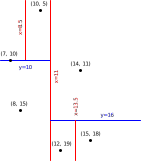
\includegraphics[width = 1 \textwidth]{figures/example_kd_plane}
		\end{minipage}
		\hspace{0.1cm}
		\begin{minipage}{0.58 \textwidth}
			\includegraphics[width = 1 \textwidth, trim=1cm 1cm 1cm 1cm, clip]{figures/example_kd}
		\end{minipage}
	\end{center}
	\caption[Example k-d tree.]{A k-d created from six vertices (left panel) and its graph representation (right panel).
		The vertices are drawn as black circles, the vertical and horizontal splitting planes
		are shown in red and blue, respectively.
		The splitting planes are written out explicitly to emphasise that a
		k-d tree is also a BSP tree (but not necessarily vice versa).
		The graph has been drawn using the \textit{Dot} tool from the \textit{Graphviz} software \cite{Ellson2003}.
		\label{fig:example_kdtree}}
\end{figure}


\paragraph{R tree}
R tree stands for \textit{rectangle tree} and is named for its use of (hyper-)rectangles 
grouping objects \cite{wiki_rtree}.
Each node in the tree has a hyperrectangle assigned to it, which serves as axis-aligned bounding box
for all the objects it contains in its child nodes. 
The tree is not necessarily a binary tree, in fact, the number of children that each node can have is 
a configuration parameter. 
The rectangular bounding boxes for the nodes at the same height may overlap, and the key to efficiency 
in this kind of tree is a good insertion algorithm which minimises such a overlap.
The most prominent of these overlap-minimised data structures is the so-called \textit{R* tree} \cite{wiki_rstartree}.
Fig. \ref{fig:example_rtrees} shows a comparison between a classical R tree and and R* tree for the
same vertex sites. The R trees shows a clearly more pronounced overlap than the R* tree.

\begin{figure}[h]
	\begin{center}
		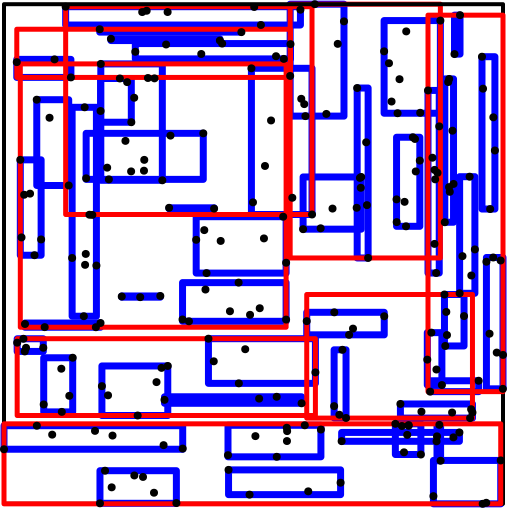
\includegraphics[width = 0.38 \textwidth]{figures/rtree8}
		\hspace{1cm}
		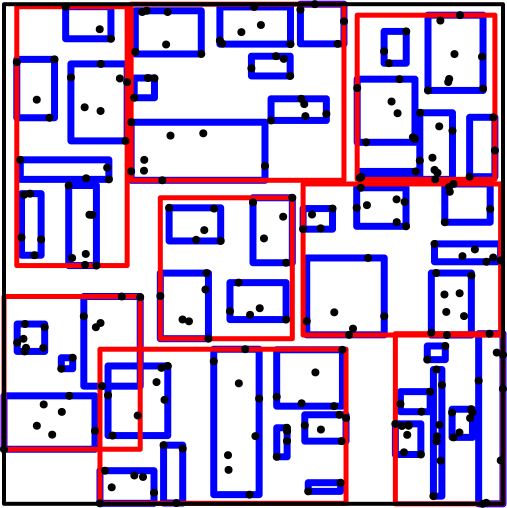
\includegraphics[width = 0.38 \textwidth]{figures/rstartree8}
	\end{center}
	\caption[Example R trees.]{An R tree (left panel) and an R* tree (right panel) for the 
		same 250 random, linearly distributed vertices (back circles). 
		The rectangular bounding boxes at each level of the R trees are marked in different colours, 
		the innermost rectangles are blue, the next level is red, and the outermost level 
		(at the root node) is black.
		The trees were created so that each node has maximally 8 children.
		These panels were calculated using the \lstinline[language=C++]|rtree| class \cite{web_boost_geometry_rtree}
		of the \textit{Boost.Geometry} library \cite{web_boost_geometry}.
		\label{fig:example_rtrees}}
\end{figure}


\subsection{Software libraries}
BSP trees are very popular in the field of computer graphics, and free and open-source implementations are 
readily available \cite{web_bsp_faq}. Unfortunately and surprisingly, the \textit{Boost} C++ libraries \cite{web_boost},
which is the preferred ressource for data types and algorithms in this work, do not feature one. 
Equally surprisingly, the \textit{Qt} libraries do feature a BSP tree implementation, but it is not part of 
their public API, but only used internally in the \lstinline[language=C++]|QGraphicsScene| class \cite{web_QGraphicsScene}.

Open-source k-d tree implementations can be found in \textit{OpenCV} \cite{web_opencv} 
and in \textit{CGAL} \cite{web_cgal}.

A high-quality implementation of R and R* trees as well as the insertion, deletion, and querying algorithms 
operating on them is readily available through the \textit{Boost.Geometry} library \cite{web_boost_geometry, web_boost_geometry_rtree}. As first tests could directly confirm the good performance of \textit{Boost.Geometry}'s,
R and R* tree codes, we will employ them for this work.



\section{Summary}
With the concept of the Voronoi diagram, basic graph theory, and spatial index trees, 
this chapter presented the foundations on which the path-mesh calculation and path-finding
algorithm of this work will be based. The following chapter will review different kinds
of path-finding methods and use parts of these to construct a bespoke method which
is suitable for the angular movement of triple-axis spectrometers.

%
% path-finding
% @author Tobias Weber <tweber@ill.fr>
% @date 2021
% @license see 'LICENSE' file
%
\chapter{Path-finding and Algorithm Overview}

This chapter is devoted to the development of the theoretical frameworks for path-finding in a triple-axis spectrometer (TAS). 
The path should furthermore be optimal in the sense that the instrument not only avoids obstacles like walls or equipment in 
the experimental area, but also keeps a maximum distance from them.

Before looking at the situation with TAS in section \ref{sec:tasrobot}, we shortly review the ideas of motion planning for a 
point-like robot in section \ref{sec:pointrobot}.



\section{Motion planning for a point-like robot}
\label{sec:pointrobot}

\subsection*{Sector-based method}
An algorithm for motion planning in a point-like robot based on decomposing the available space into sectors is 
given in Ref. \cite[Ch. 13, pp. 283-306]{Berg2008}, whose descriptions we follow in this section. 
While the book chapter also describes polygonal robots, we limit ourselves to the parts of the chapter 
that are relevant for the present work.

The movement of the point-like robot in question is not restricted to conventional Cartesian space, its coordinates are given in configuration
space  \cite[Ch. 13.1, pp. 284-286]{Berg2008}, which comprises its inherent degrees of freedom and can -- for instance -- include angular motion.

The algorithm consists of two parts: First, the separation of allowed space into sectors, within which the robot can move 
without hitting an obstacle \cite[p. 286]{Berg2008}. 
The second part concerns the computation of the actual path and is given in Ref. \cite[p. 289]{Berg2008}. 
In the first part, a trapezoidal map (explained below) is created for the configuration space containing the obstacles, 
both of polygonal shape. The trapezoids inside the obstacles are removed form the final map as the robot has to stay clear 
of them. The second part of the algorithm calculates the path of the robot by finding the trapezoids which contain the start 
and goal points, and finding the edges between adjacent trapezoids from starting to ending trapezoid via a breadth-first search in the 
trapezoidal map. The robot will thus first move to the centre of its containing trapezoid, followed by the centre of an edge connecting 
the current to the next trapezoid, next to the centre of the next trapezoid, and so forth until it arrives at its goal. 
The situation is depicted in Fig. \ref{fig:robot_trapezoids}, where we restrict ourselves to line-like obstacles for simplicity, effectively
only using the second part of the algorithm.

Trapezoidal maps and the algorithm for their calculation are given in Ref. \cite[Ch. 6, pp. 121-146]{Berg2008}. Basically, the map of
trapezoids is obtained by extending vertical lines from every vertex in a collection of line segments. The vertical
extensions reach out until they intersect with another line segment of the collection, or an outer bounding box. The original line 
segment and the intersected segment on top (or bottom, respectively) together with the vertical lines form a trapezoid, as shown in 
Fig. \ref{fig:robot_trapezoids}. Together with the trapezoid map, the algorithm constructs in $O \left(n \log_{2} n \right)$ time a data 
structure, which allows querying for the trapezoid containing a given point with time complexity $O \left( \log_{2} n \right)$, 
where $n$ is the number of line segments \cite[Theorem 6.3, p. 133]{Berg2008}.

\begin{figure*}[htb]
	\centering
	\includegraphics[width = 0.4 \textwidth]{figures/pointrobot_walls.pdf}
	\hspace{1 cm}
	\includegraphics[width = 0.4 \textwidth]{figures/pointrobot_walls_trapezoids.pdf}
	\caption{Left panel: A point-like robot has to find a way around line segments which represent obstacles. Right panel: 
		The algorithm outlined in Ref. \cite[p. 289]{Berg2008} constructs a trapezoid map and moves the robot on the
		shortest path from the centre of one trapezoid to the centre of the edge connecting to the next trapezoid, to the
		centre of that trapezoid, and so forth (blue arrows).}
	\label{fig:robot_trapezoids}
\end{figure*}

While the present algorithm can be extended towards polygonal robots \cite[Ch. 13.3, pp. 290-297]{Berg2008} and provides
some useful ideas, it has several severe drawbacks. First and foremost, the trapezoid map cannot handle the case when
two or more line segment vertices coincide, making it very difficult to model polygonal obstacles and not only using mere
line segments. Second, our own implementation has shown that for the algorithm to be stable, it has to handle many 
special cases, for example to eliminate vertices with equal $x$ coordinate components or vertical lines.

\vspace{0.5cm}

\subsection*{Retraction method}
Apart from decomposing the available configuration space into sectors, a more direct approach can be taken. This
approach is called the retraction method and is based on constructing the Voronoi regions (see \ref{ch:voronoi})
of the obstacles and moving the robot along the Voronoi edges, which ensures that the path is optimal in the
sense that the robot is always at the farthest distance from any obstacle \cite[pp. 163 and 304]{Berg2008}.
An example path for the same problem as before is given in Fig. \ref{fig:robot_voronoi}.
It is this approach we will follow for TAS motion planning.

\begin{figure}[htb]
	\centering
	\includegraphics[width = 0.4 \textwidth]{figures/pointrobot_walls_voronoi.pdf}
	\caption{The accessible configuration space is subdivided into the Voronoi regions of the obstacles (coloured). The optimal
		path (blue arrows) in the sense that it keeps the robot at maximum distance from any obstacle, has it move along the 
		Voronoi edges.}
	\label{fig:robot_voronoi}
\end{figure}



\section{Motion planning for a triple-axis spectrometer}
\label{sec:tasrobot}

As it is imperative that the instrument not move into any walls, we choose the retraction method using the obstacles' Voronoi regions.
As for a TAS several coordinate systems are available, we have several equivalent possibilities to describe its movement. 

\subsection*{Instrument positions configuration space}
The first possibility would be to model the entire instrument as a polygonal robot arm and directly use the position of the robot as
its configuration space. This way it would be directly possible to use a polygonal representation of the walls and construct their
Voronoi regions -- or even trapezoidal maps -- as discussed in Sec. \ref{sec:pointrobot}. The main problem with this approach is the
very complicated treatment necessary for the instrument itself.

\subsection*{Crystal coordinates configuration space}
A better way is to use a configuration space where the instrument is represented as a single point in that space. This comes at the 
cost of the shape of the walls becoming more complicated when transformed into configuration space, 
they may not even be simply-connected anymore in that space. There
are two choices for such a configuration space: We can either use the reciprocal crystal coordinates as discussed in Ch. \ref{ch:xtal}
or use a configuration space comprised of the instrumental angles.

Using the reciprocal crystal coordinates as configuration space would need a transformation of the walls into the four-dimensional
reciprocal space (three momentum and on energy coordinate). Even when taking into account that the TAS is usually restricted
to a two-dimensional scattering plane, thereby dropping one of the momentum dimensions, the problem would still be 
three-dimensional.

\subsection*{Angular configuration space}
On the other hand, using the instrument angles seems to be even more complicated at first glance. The instrument comprises
six angles, namely the crystal and scattering angles for the monochromator, the sample and the analyser crystals, respectively,
leading to a six-dimensional configuration space. When can take into account that not all angles are independent of one another:
The monochromator and analyser scattering angles are always double their respective crystal angles, because they both
have to fulfill the Bragg condition. We are therefore left with four independent angles: the monochromator and analyser 
scattering angles as well as the sample crystal and scattering angle. 

We are mainly interested in collisions of the instrument with walls or itself, this way the sample crystal angle can be dropped 
from the analysis, because it only rotates the sample axis, but does not move the instrument. It can still lead to forbidden 
positions if it rotates too far and rips out cables or tubes, but these cases we can treat as their own one-dimensional problem. 

A further simplification is possible when taking into account that during a typical experiment the instrument usually only moves 
either its monochromator or analyser angle to choose the energy transfer, but not both. Therefore, one of these angles, 
usually the analyser angle, rests at a constant value. In total, we are left with a two-dimensional configuration space comprised 
of the monochromator and the sample scattering angle. A typical situation is shown in Fig. \ref{fig:tas_wall}. Here, the instrument 
motion is blocked by an obstacle in the experimental zone. The configuration space image shows that the obstacle transforms
into a non-primitive geometric object in configuration space, which -- as already mentioned -- does not even have to be
simply-connected.

\begin{figure}[htb]
	\centering
	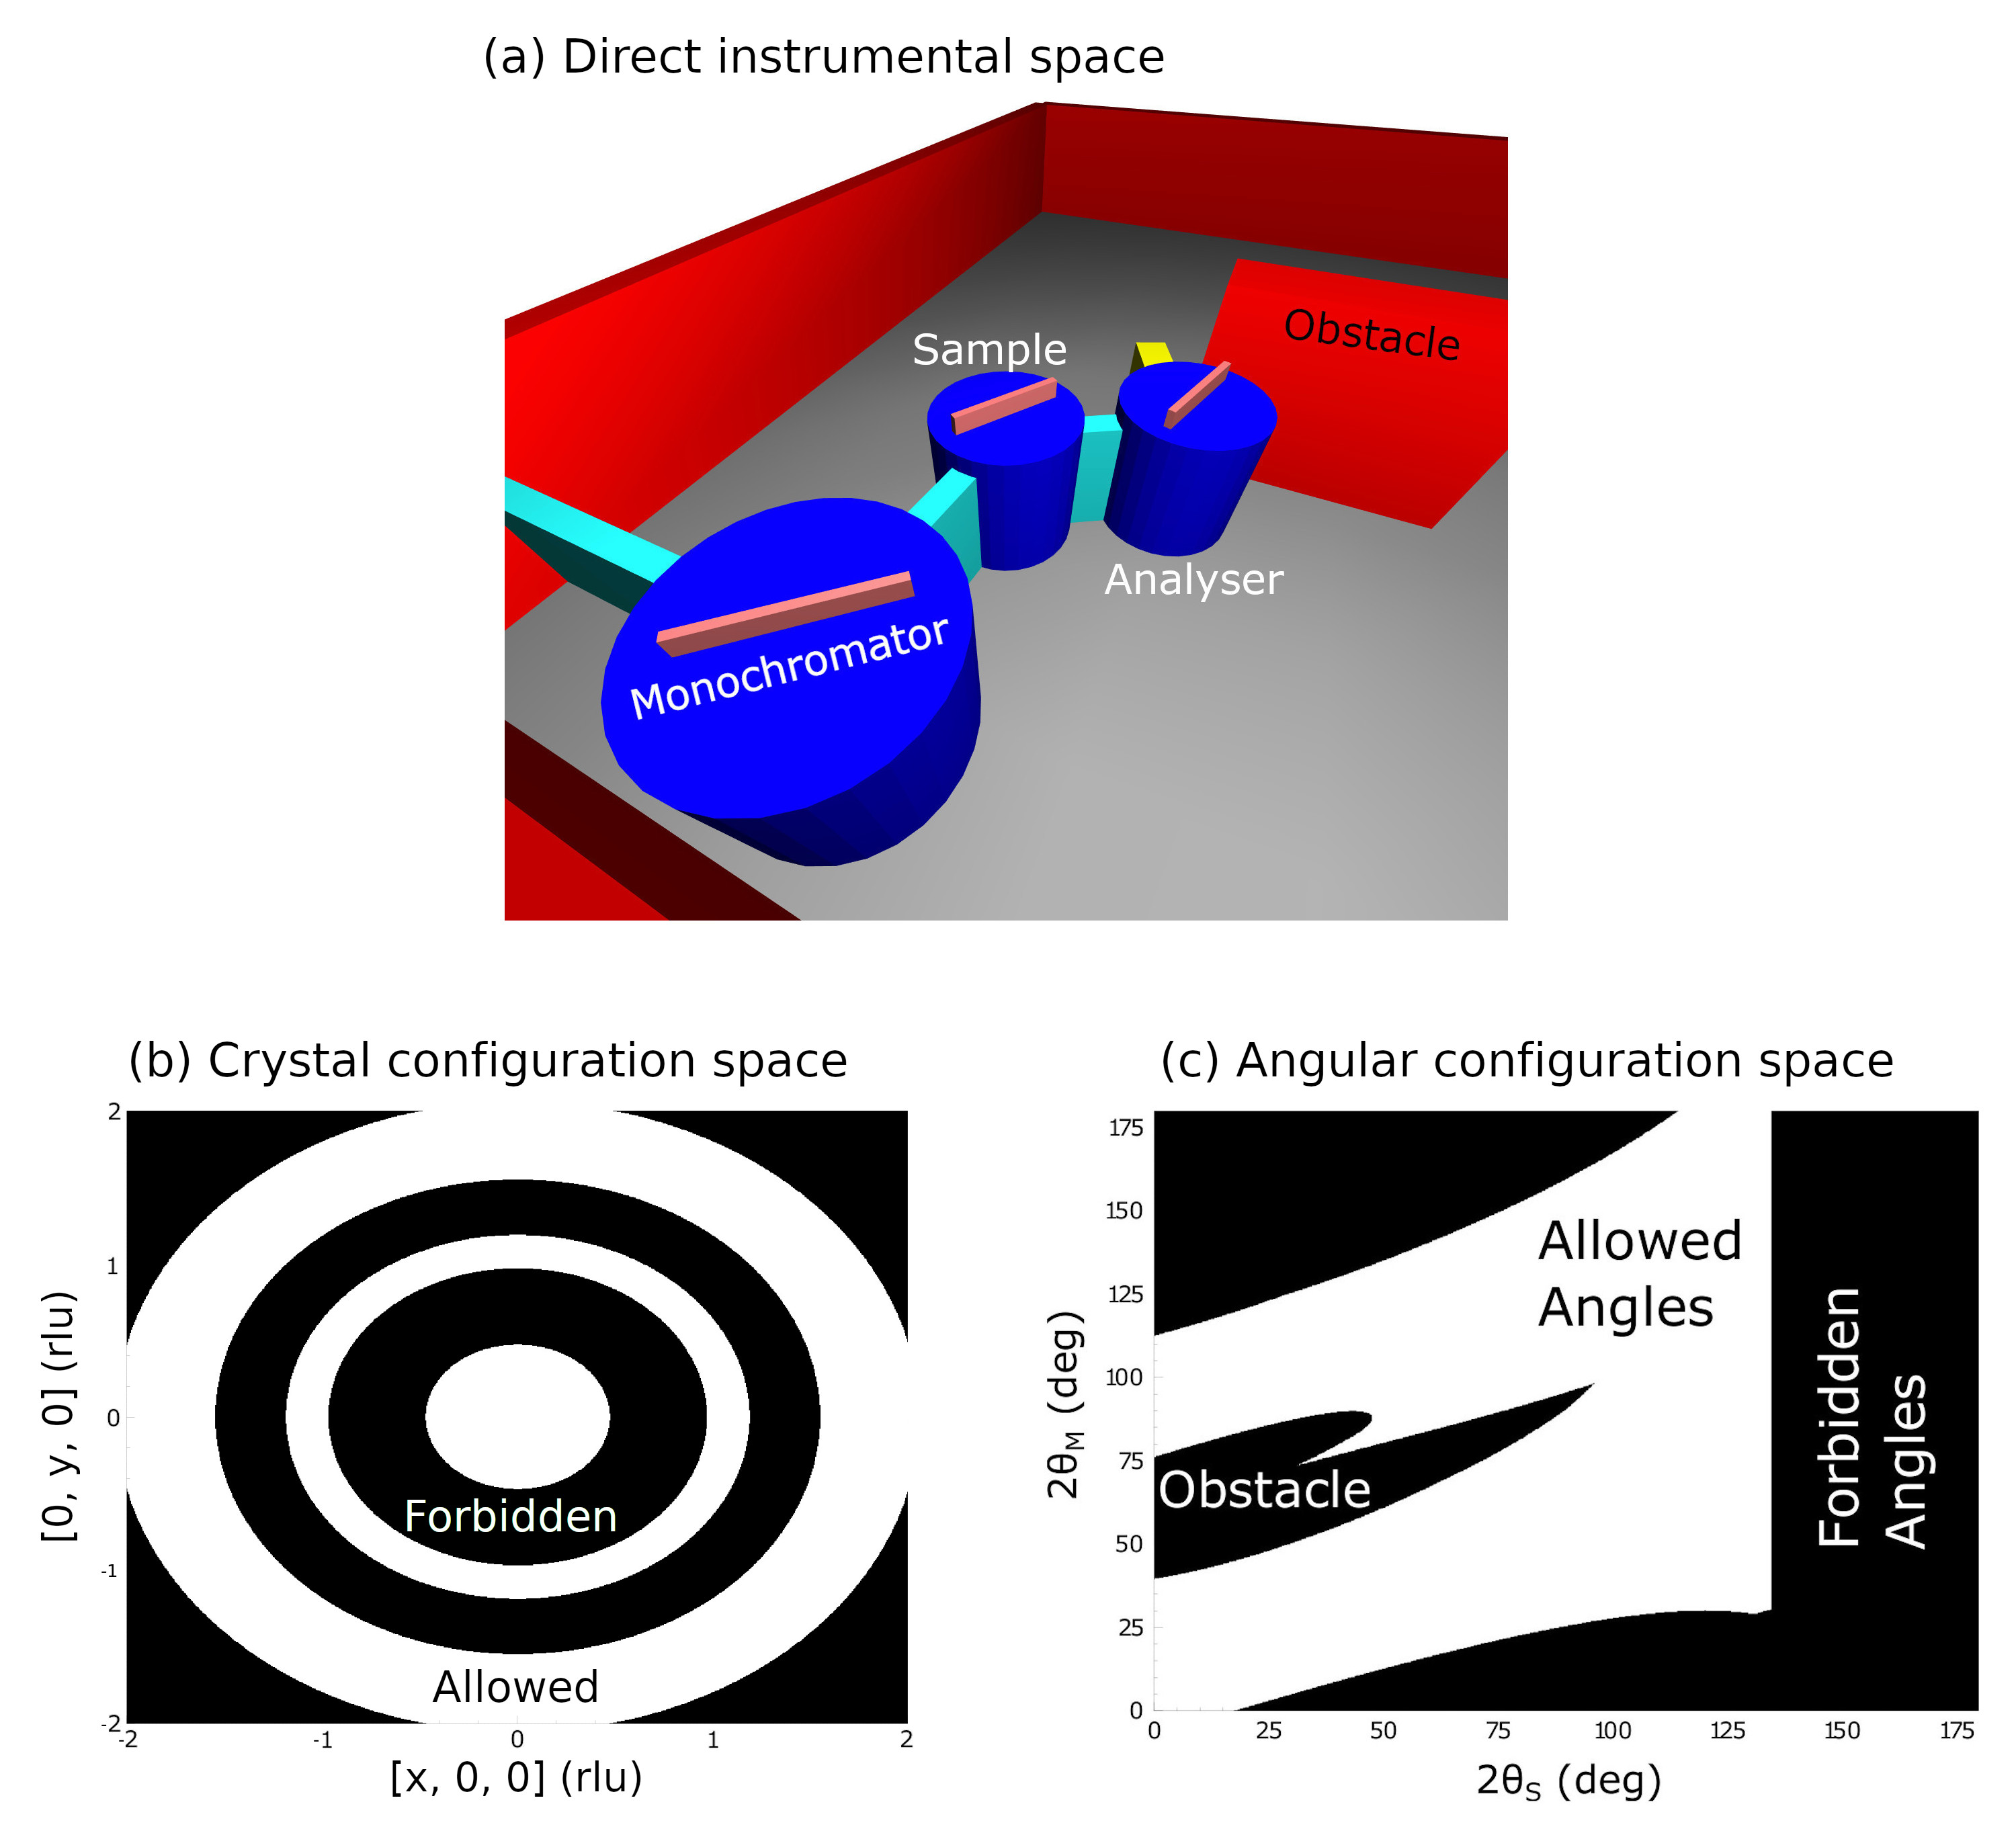
\includegraphics[width = 0.95 \textwidth]{figures/tas_wall.jpg}
	\caption{An obstacle as it appears in the instrument space (left) and in the angular configuration space (right). 
		In the configuration space, allowed instrument angular positions are shown in white, forbidden positions in black. 
		The outer areas of disallowed positions are given either by collisions of the instrument with the outer walls or 
		with itself.}
	\label{fig:tas_wall}
\end{figure}


\subsection*{Overall strategy}

The strategy for planning the motion of the spectrometer comprises several steps. Modifying the algorithm for
a point-like robot described in Ref. \cite[Ch. 13, pp. 283-306]{Berg2008} (see Sec. \ref{sec:pointrobot}), we summarise the
steps here before describing them in detail together with the actual implementation in the next chapter.

Two tasks are needed. The first task is building the possible paths the instrument can move along. The second task contains the movement of the instrument on the generated paths. The two tasks comprise these following steps:
\begin{enumerate}
	\item Building the path.
	\begin{enumerate}
		\item Calculate the angular configuration space as described above.
		\item Trace the obstacle contours in angular configuration space. This step is necessary because they can be of arbitrary
			shape in this representation and are not necessarily geometric primitives, as seen in Fig. \ref{fig:tas_wall}.
		\item Approximate the traced contour curves with line segments.
		\item Simplify the line segments. This is necessary because the line segments generated in the previous step are not optimal:
			First, they may contain back-to-back collinear lines which can be unified. Second, jagged edges and zigzag lines may be
			produced in practice. These need to be eliminated or at least smoothed before the next step.
		\item Split all polygonal line segments that build up the contours into convex regions. With this we can group all lines
			in a convex region and only calculate the Voronoi diagrams for these groups instead of all line segments.
		\item Calculate the Voronoi diagram (see Ch. \ref{ch:voronoi}) for the line segment groups. The Voronoi edges are the
		possible instrument paths in configuration space. Save both the Voronoi diagram as well as its representation in a graph structure.
		\item Simplify the Voronoi diagram. For example, Voronoi vertices and edges inside obstacle regions have to be removed.
			These are generated in the previous step because, there, no differentiation was made between the ``inside'' and
			``outside'' regions of the convex line segment contour groups.
	\end{enumerate}

	\item Executing the instrument motion.
	\begin{enumerate}
		\item Convert the given crystal coordinates into instrument coordinates.
			The user of a triple-axis spectrometer usually enters the coordinates in the crystal coordinate system
			(see Ch. \ref{ch:xtal}). The start and end point of the instrument path have to be converted from crystal
			coordinates into instrument angles. The instrument angles form a coordinate point in angular configuration
			space.
		\item Determine the Voronoi regions of the start and end coordinate points.
		\item Move the instrument to the edge of the start Voronoi region.
		\item Calculate the shortest path to the edge of the Voronoi region containing the end point using Dijkstra's algorithm
			(see Ch. \ref{ch:dijkstra}) and move the instrument along that path.
		\item Move the instrument from the edge of the Voronoi region containing the end point towards that point.
	\end{enumerate}
\end{enumerate}

%
% path-finding
% @author Tobias Weber <tweber@ill.fr>
% @date 2021
% @license see 'LICENSE' file
%

\chapter{Path-finding Details and Implementation}
\label{ch:impl}

In this chapter we describe the individual steps of the strategy (see p. \pageref{sec:strategy}) in detail
and present an implementation in C++ \cite{Stroustrup2008, Stroustrup2018}. Specifically,
the latest version 20 of the C++ standard \cite{ISOCPP20} was employed in the creation of the software
together with the Boost C++ template libraries \cite{web_boost}. The source code for the implementation
can be found in the directory \lstinline|./src/core| together with the library routines in \lstinline|./src/libs|
of the repository at \url{https://code.ill.fr/scientific-software/takin/paths}. Stable versions of the
source code have furthermore been registered under the DOI \href{https://doi.org/10.5281/zenodo.4625649}{10.5281/zenodo.4625649}.

Section \ref{sec:tasmodel} is dedicated to modelling the triple-axis spectrometer (TAS), 
section \ref{sec:buildpath} discusses the steps involved in building up the instrument path, 
and section \ref{sec:exepath} focuses on executing the instrument motion along the path.
The graphical user interface is presented separately, namely in chapter \ref{ch:gui}.





% -----------------------------------------------------------------------------
% instrument model
% -----------------------------------------------------------------------------
\section{TAS instrument modelling}
\label{sec:tasmodel}

The instrument space comprising the triple-axis spectrometer, the walls and obstacles as well as the floor is modelled in
the class \lstinline[language=C++]|InstrumentSpace|. It also serves as high-level interface for loading and saving
the instrument geometry and states, signalling mechanisms for state changes using the publish-subscribe mechanism
via Boost.Signals2 \cite{web_boost_signals}, as well as checking the instrument for collisions.

The classes \lstinline[language=C++]|Instrument| and \lstinline[language=C++]|Axis| contain the actual instrument definition.
The spectrometer is modelled as a hierarchy of the three principal axes, namely monochromator, sample and analyser.
Each axis has three local coordinate systems, namely the rotation relative to the incoming and outgoing vector, respectively,
and an internal rotation which is decoupled from the other local rotations.
Geometrical objects are derived from the abstract, purely virtual class \lstinline[language=C++]|Geometry| and can be
coupled to any of these three local coordinate systems.
This makes it possible to model neutron-optical components attached to the either the incoming or outgoing path of the
neutron beam at the specific axis. It furthermore makes it possible to have components which rotate independently of
the axis.
Physically, the outgoing coordinate system is equal to the scattering angle, while the internal angle corresponds
to the crystal rocking angle (see Ch. \ref{ch:xtal}).
The transformation matrices corresponding to the three local coordinate systems are calculated as follows:

\begin{equation}
\begin{split}
	T_{\mathrm{in}}^{i} & \ =\  T_{\mathrm{out}}^{i-1} \cdot P^{i} \cdot R\left(\theta_{\mathrm{in}}^{i}\right), \\
	T_{\mathrm{int}}^{i} & \ =\  T_{\mathrm{in}}^{i} \cdot R\left(\theta_{\mathrm{int}}^{i}\right), \\
	T_{\mathrm{out}}^{i} & \ =\  T_{\mathrm{in}}^{i} \cdot R\left(\theta_{\mathrm{out}}^{i}\right).
\end{split}
\end{equation}

Here, $T_{\mathrm{in,\, int,\, out}}^{i}$ names the transformation matrices of the incoming, internal (decoupled) and outgoing
coordinate system of axis $i$, respectively.
$T_{out}^{i-1}$ is the outgoing transformation of the preceding instrument axis, or the identity if it is the first axis in the hierarchy.
$R\left(\theta_{\mathrm{in,\, int,\, out}}\right)$ are the corresponding rotation matrices and $P^i$ is the translation
of the local coordinate origin of the respective axis $i$.
The situation is depicted in Fig. \ref{fig:tas_axes}.


\begin{figure*}
	\begin{minipage}{0.45 \textwidth}
		\begin{center}
			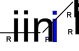
\includegraphics[width = 0.75 \textwidth]{figures/axis}
		\end{center}
	\end{minipage}
	%\hspace{1cm}
	\begin{minipage}{0.45 \textwidth}
		\begin{center}
			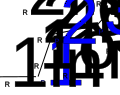
\includegraphics[width = 0.95 \textwidth]{figures/axes}
		\end{center}
	\end{minipage}
	\caption{Left panel: Local transformations for an axis. The symbols $R_{\mathrm{x}}^i$ are shorthands
	for the rotation matrices $R\left( \theta_{\mathrm{x}}^i \right)$, with $x = \left\{ \mathrm{in,\, int,\, out} \right\}$.
	$P^i$ is the point of origin for the axis.
	Right panel: Three coupled axes build up the triple-axis spectrometer, with axes 1, 2, and 3 naming the monochromator,
	the sample, and the analyser axis, respectively.
	\label{fig:tas_axes}}
\end{figure*}

% -----------------------------------------------------------------------------





% -----------------------------------------------------------------------------
% path building
% -----------------------------------------------------------------------------
\section{Path-building}
\label{sec:buildpath}

As discussed in chapter \ref{sec:tasrobot}, path-creation will be based on the angular configuration space
(as opposed to -- for example -- crystal configuration space). The top-level C++ class for creating the path
is named \lstinline[language=C++]|PathBuilder|. It mainly calls the low-level routines from the geometry
library situated in the directory \lstinline|./src/libs| of the source code repository.


\subsection{Angular configuration space}
As the obstacles do not have any geometrically primitive shape in angular configuration space, we iterate
through the configuration space on a two-dimensional grid and create a bitmap of allowed and forbidden
positions. The grid extends towards the scattering angles $2\theta_S \in \left[ -180^{\circ},\, 180^{\circ} \right]$ and monochromator angles of $2\theta_M \in \left[0^{\circ},\, 180^{\circ} \right]$, where, for the monochromator, we do
not the full angular range as this is not possible in real instruments which has the monochromator at a fixed position
and only scatters in one direction. The sample scattering angle, on the other hand, needs the full angular range as
scattering on both sides of the axis is done in practice.

To check for the allowed positions, the instrument model as described in sec \ref{sec:tasmodel} is moved to
each $\left( 2\theta_S,\, 2\theta_M \right)$ position on the grid and tested for collisions with the walls or with
itself. Even though the instrument model itself is a three-dimensional representation of the spectrometer, we
can nevertheless simplify the collision detection checks to a two-dimensional plane. The reason for this is
that all possible obstacles in the instrument path, for instance walls and pillars, are upright and do not have
any sloped angles. The same is true for the instrument itself.

Collision calculation on the two-dimensional grid is spread out on several processor cores using 
the \lstinline[language=C++]|thread_pool| \cite{web_boost_asio_threadpool} class from the 
Boost.Asio \cite{web_boost_asio} asynchronous input/output library.


\subsection{Contour tracing}


\subsection{Line-segment generation and simplification}


\subsection{Generation of convex regions}


\subsection{Calculation of the Voronoi diagram}
\label{sec:voronoi}


\subsection{Simplification of the Voronoi diagram}


% -----------------------------------------------------------------------------





% -----------------------------------------------------------------------------
% instrument motion
% -----------------------------------------------------------------------------
\section{Instrument movement}
\label{sec:exepath}


\subsection{Determination of the start and end coordinates}



\subsection{Calculation of Dijkstra's shortest path}
\label{sec:dijkstra}


% -----------------------------------------------------------------------------

%
% gl
% @author Tobias Weber <tweber@ill.fr>
% @date aug-2021
% @license see 'LICENSE' file
%

\chapter{Interlude: Mathematics for 3-d Graphics}
\label{ch:gl}

The software of this work uses \textit{OpenGL} \cite{web_OpenGL} for visualisation in its main graphical user interface (GUI).
Before discussing the main GUI proper, this chapter reviews concepts behind three-dimensional graphics in a general way.
Here, we mainly describe the most important mathematical aspects of 3-d graphics, a comprehensive overview of 
\textit{OpenGL} and the mathematics involved can be found in Ref. \cite{Sellers2002}.



\section{Coordinate systems and transformations}
To draw a three-dimensional object onto the screen, several principal coordinate systems are typically maintained,
namely the local coordinate system of the 3-d object, a global coordinate system common for all objects in the scene, the
system of the camera, as well as screen (device) and window coordinates \cite[pp. 63-66]{Sellers2002}.
The vertices of the 3-d object, $\left|x\right>$, are thus transformed into a window's 2-d pixels by using four
matrices transforming from one coordinate system to the next,
\begin{equation}
	\boxed{\left|x_{\mathrm{window}}\right> \ =\ W \cdot P \cdot V \cdot  M \cdot  \left| x_{\mathrm{model}} \right>,}
	\label{eq:gl_mvp}
\end{equation}
where $M$ is a matrix transforming the model's local system (used, for example, to spin the object around one of
its axes) into the global coordinate system of the scene. $V$ is the view matrix given by the camera's coordinate system
which transforms global object coordinates into the camera's viewing frame. These matrices take the form
described in section \ref{sec:gl_trafos}.
$P$ projects the three-dimensional scene onto the two-dimensional plane representing the screen \cite{web_gl_ortho, web_gl_perspective} and is described in section \ref{sec:gl_projs}. 
Finally, $W$ is the window or viewport matrix which scales and translates the projected screen coordinates 
into the pixel coordinates of the display window \cite{web_gl_viewport}, it is discussed in section \ref{sec:gl_viewport}.

Historically, \textit{OpenGL} used a fixed transformation and lighting pipeline \cite{wiki_gl_history} for
these transformations. The pipeline maintained different stacks of matrices for the combined model-view and
projection matrices \cite{web_gl_matrixmode}.
Modern \textit{OpenGL} \cite{web_OpenGL} versions do not use internal matrix stacks anymore, instead all
transformation and lighting operations of the rendering pipeline are programmable through small \textit{shader}
programs that are directly executed on the graphics processing unit (GPU) \cite{wiki_gl_history}
and are written in a \textit{C}-like language \cite{wiki_glsl}.
Going even further than \textit{OpenGL}, its successor \textit{Vulkan} \cite{web_Vulkan} makes the pipeline
itself dynamic and programmable, not only the shaders of its individual steps, but sacrificing the ease of use in 
exchange for flexibility.
While the transformation given by Eq. \ref{eq:gl_mvp} is not fixed anymore, its form is usually maintained
in the shaders by the user. More information on the rendering pipeline and the shaders is given in 
section \ref{sec:gl_shaders}.

\paragraph{Object selection}
The transformation inverse to Eq. \ref{eq:gl_mvp} is also of importance, namely to be able to select objects in the
three-dimensional scene by mouse. 
To that end, a line is calculated by ``unprojecting'' two homogeneous $\left|x_{\mathrm{window}}\right>$ vectors
(see next section) having the same mouse position as their $x$ and $y$ components and the distance of the
near and far planes of the so-called view frustum (see section \ref{sec:gl_perspective_proj})
as two different $z$ coordinate components.
Finally, the intersection of the line through these two unprojected $\left|x_{\mathrm{model}}\right>$ points 
with the scene geometry is calculated. 
The unprojection operation as the inverse of Eq. \ref{eq:gl_mvp} is given by \cite{web_gl_unproject}:
\begin{equation}
	\left|x_{\mathrm{model}}\right> \ =\ M^{-1} \cdot V^{-1} \cdot P^{-1} \cdot  W^{-1} \cdot  \left| x_{\mathrm{window}} \right>,
\end{equation}
and normalising $\left|x_{\mathrm{model}}\right>$ by its fourth (homogeneous) component \cite{web_gl_unproject}.



\section{3-d transformations}
\label{sec:gl_trafos}
To simplify the calculations when translations are involved, \textit{OpenGL} uses homogeneous coordinates.
Homogeneous coordinates append a fourth component to the three-dimensional vectors, which is set to zero for
directions and non-zero for vertices, where the original vertex coordinates are recovered by normalising this
fourth component to one \cite[pp. 235, 357]{Bronstein2008}. Homogeneous coordinates help describing translations
in matrix form, and projective division using the normalisation operation by the fourth component, as will be
described next.


% -----------------------------------------------------------------------------
% scaling
% -----------------------------------------------------------------------------
\subsection{Translation}
Using homogeneous coordinates, vertices can be translated by left-multiplying with a 
matrix whose fourth column represents the translation vector \cite{web_gl_translate}:
\begin{equation}
	\left( \begin{array}{c} x + t_x \\ y + t_y \\ z + t_z \\ 1 \end{array} \right) 
	\ =\  
	\left( \begin{array}{cccc} 
		1 & 0 & 0 & t_x \\
		0 & 1 & 0 & t_y \\
		0 & 0 & 1 & t_z \\
		0 & 0 & 0 & 1
	\end{array} \right) \cdot
	\left( \begin{array}{c} x \\ y \\ z \\ 1 \end{array} \right).
\end{equation}
Note that direction vectors, which have their fourth component zero, are not affected by a translation.
% -----------------------------------------------------------------------------


% -----------------------------------------------------------------------------
% scaling
% -----------------------------------------------------------------------------
\subsection{Scaling}
By the same token, scaling along the principal axes is performed by setting the diagonal matrix 
elements \cite{web_gl_scale}:
\begin{equation}
	\left( \begin{array}{c} s_x \cdot x \\ s_y \cdot y \\ s_z \cdot z \\ 1 \end{array} \right) 
	\ =\  
	\left( \begin{array}{cccc} 
		s_x & 0 & 0 & 0 \\
		0 & s_y & 0 & 0 \\
		0 & 0 & s_z & 0 \\
		0 & 0 & 0 & 1
	\end{array} \right) \cdot
	\left( \begin{array}{c} x \\ y \\ z \\ 1 \end{array} \right).
\end{equation}
% -----------------------------------------------------------------------------


% -----------------------------------------------------------------------------
% rotation
% -----------------------------------------------------------------------------
\subsection{Rotation}
The set of rotations in three-dimensional space forms an algebraic group, the special orthogonal group $\mathrm{SO\left(3\right)}$,
which comprises all orthogonal matrices with determinant 1 \cite[pp. 849-851]{Arfken2013}.
There are two popular ways to describe rotations $R \in \mathrm{SO\left(3\right)}$ given the rotation axis and angle, 
namely the Rodrigues formalism and quaternions. 
% As they are both ubiquitous in computer graphics, we describe each of them briefly in the following paragraphs.
For clarity, we only write out the left-upper 3x3 part of the homogeneous 4x4 matrices.


\subsubsection{Rodrigues formalism}
For the derivation in this section we follow Refs. \cite[p. 718, p. 816]{Arens2015} and \cite{wiki_rodrigues}.
The matrix $R$ describing the rotation about a normalised vector $\left|v\right>$ under an angle $\alpha$ can be decomposed into
three projections onto the rotated coordinate system \cite[p. 718, p. 816]{Arens2015}:
\begin{equation}
	\boxed{R \ = \ P_{||} + P_{\perp} \cos \alpha + P_{\times} \sin \alpha.}
	\label{eq:rodrigues}
\end{equation}
Here, $P_{||}$ is the projector onto the axis itself, which remains invariant under a rotation and is written as \cite[p. 814]{Arens2015}:
\begin{equation}
	P_{||} \ =\ \left|v\right> \left<v\right| \ =\ 
		\left( \begin{array}{ccc} 
			v_1^2   &    v_1 v_2 &       v_1 v_3 \\
			v_2 v_1 &      v_2^2 &       v_2 v_3 \\
			v_3 v_1 &    v_3 v_2 &         v_3^2
		\end{array} \right).
\end{equation}
To see that this is the case, one can apply a the projector to a test vector $\left| x \right>$ resulting in $\left|v\right> \left<v | x \right>$,
which is the projection of $\left| x \right>$ onto $\left| v \right>$ in the direction of $\left| v \right>$ \cite[p. 814]{Arens2015}.

The second axis for rotation is found by applying $P_{\perp}$, the orthogonal projector onto the plane, 
whose normal is given by $\left|v\right>$, and which reads \cite[p. 814]{Arens2015}
\begin{equation}
	P_{\perp} \ =\ 1 - \left|v\right> \left<v\right| \ =\ 
		\left( \begin{array}{ccc} 
			1 - v_1^2    &      - v_1 v_2 &         - v_1 v_3 \\
			   - v_2 v_1 &      1 - v_2^2 &         - v_2 v_3 \\
			   - v_3 v_1 &      - v_3 v_2 &         1 - v_3^2
		\end{array} \right).
\end{equation}
Here, $1$ names the unit matrix, and the equation is derived from completeness relation of the vector space under
a basis $\left| v_i \right>$ \cite[p. 814]{Arens2015}:
\begin{equation}
	1 \ =\  \sum_i \left| v_i \right> \left< v_i \right|.
\end{equation}

Finally, the third axis is found by applying $P_{\times}$, the skew-symmetric matrix for $\left|v\right>$.
This is the matrix which -- when applied to a vector $\left|x\right>$ -- gives the cross product of $\left|v\right>$ and $\left|x\right>$, 
and it reads \cite{wiki_skewsymm}:
\begin{equation}
	P_{\times} \ =\ 
		\left( \begin{array}{ccc} 
			0     & -v_3 &  v_2 \\
			v_3   & 0    & -v_1 \\
			-v_2  & v_1  & 0
		\end{array} \right).
\end{equation}

Explicitly writing Eq. \ref{eq:rodrigues} thus yields the full Rodrigues formula \cite[p. 718, p. 816]{Arens2015}:
\begin{equation}
	R \ = \ 
		\left( \begin{array}{ccc} 
			v_1^2   &    v_1 v_2 &       v_1 v_3 \\
			v_2 v_1 &      v_2^2 &       v_2 v_3 \\
			v_3 v_1 &    v_3 v_2 &         v_3^2
		\end{array} \right)
	+ 	\left( \begin{array}{ccc} 
			1 - v_1^2    &      - v_1 v_2 &         - v_1 v_3 \\
			   - v_2 v_1 &      1 - v_2^2 &         - v_2 v_3 \\
			   - v_3 v_1 &      - v_3 v_2 &         1 - v_3^2
		\end{array} \right)
		\cos \alpha 
	 + 
		\left( \begin{array}{ccc} 
			0     & -v_3 &  v_2 \\
			v_3   & 0    & -v_1 \\
			-v_2  & v_1  & 0
		\end{array} \right)
		\sin \alpha,
	\label{eq:rodrigues_expl}
\end{equation}
which is, for example, used in \textit{OpenGL}'s  \lstinline[language=C]|glRotate| functions \cite{web_gl_rotate}.

Using the canonical coordinate basis vectors $\left| x \right> = \left( 1\,0\,0 \right)^t$, $\left| y \right> = \left( 0\,1\,0 \right)^t$,
and $\left| z \right> = \left( 0\,0\,1 \right)^t$, respectively, we reproduce the well-known simple rotation matrices around the
coordinate axes as special cases \cite[p. 238]{Bronstein2008}:
\begin{equation}
	R_x \ =\ 
		\left( \begin{array}{ccc} 
			1 &            0 &            0  \\
			0 &  \cos \alpha & -\sin \alpha  \\
			0 & \sin \alpha  &  \cos \alpha
		\end{array} \right),\,
	R_y \ =\ 
		\left( \begin{array}{ccc} 
			  \cos \alpha &         0 &  \sin \alpha \\
			           0  &         1 &            0 \\
			-\sin \alpha  &         0 &  \cos \alpha
		\end{array} \right),\,
	R_z \ =\ 
		\left( \begin{array}{ccc} 
			 \cos \alpha & -\sin \alpha &             0  \\
			\sin \alpha  &  \cos \alpha &             0  \\
			           0 &            0 &             1
		\end{array} \right).
\end{equation}


\subsubsection{Quaternions}
Quaternions are hyper-complex numbers of the form $w + x \cdot i + y \cdot j + z \cdot k$, possessing one real 
component, $w$, and three imaginary components, $x$, $y$, and $z$. 
Usually, quaternions are written as tuples $\left( w,\,x,\,y,\,z \right) = \left( w,\,\underline{v} \right) \in \mathbb{H}$,
where the three imaginary components are treated as a vector component.
Algebraically, quaternions form the division ring $\mathbb{H}$, named after William Rowan Hamilton, which follows from the 
basic properties of the three imaginary units, $i$, $j$, and $k$ \cite[p. 103]{Kuipers2002}:
\begin{equation}
	i^2 \ =\ j^2 \ =\ k^2 \ =\ ijk \ =\ -1.
	\label{eq:quat_basic}
\end{equation}
A very good in-depth treatise of quaternion algebra and analysis can be found in the book by Kuipers \cite{Kuipers2002},
which we follow in this section.
Here we only present some important results, please refer to Ref. \cite{Kuipers2002} for the derivations.

\paragraph{Quaternion multiplication}
The product of two quaternions $\left( w_1,\,\underline{v_1} \right),\ \left( w_2,\,\underline{v_2} \right) \in \mathbb{H}$ 
derives from the basic algebraic property (Eq. \ref{eq:quat_basic}) and is \cite[pp. 106-110]{Kuipers2002}:
\begin{equation}
	\left( w_1, \,\underline{v_1} \right) \cdot \left( w_2, \;\underline{v_2} \right) \ \equiv \ 
	\left( w_1 w_2 - \underline{v_1} \cdot \underline{v_2}, \;\underline{v_1} \times \underline{v_2} + w_1 \underline{v_2} + w_2 \underline{v_1}\right).
\end{equation}
Multiplying a quaternion $q = \left( r,\, \underline{s} \right) \in \mathbb{H}$ with a vector 
$\underline{v} \in \mathbb{R}^3$  reduces to two quaternion multiplications and is done by \cite[p. 127]{Kuipers2002}:
\begin{equation}
	q \cdot \underline{v} \ =\ 
	q \cdot \left(0,\ \underline{v} \right) \cdot q^{*} \ =\ 
	\left( r,\, \underline{s} \right) \cdot \left(0,\ \underline{v} \right) \cdot \left( r,\, -\underline{s} \right).
	\label{eq:mult_quat_vec}
\end{equation}
where $q^{*} = \left( r,\, -\underline{s} \right)$ is the complex conjugate quaternion \cite[pp. 110-111]{Kuipers2002}.

\paragraph{SO(3)}
Representants of the special orthogonal group $\mathrm{SO\left(3\right)}$, which comprises rotations in 
three-dimensional space by an angle $\alpha$ around a normalised vector $\underline{v}$ \cite[pp. 849-851]{Arfken2013},
can be directly written in quaternion form in an analogy to Euler's formula for complex numbers \cite{wiki_quatrot}:
\begin{equation}
	\boxed{
	q_{\mathrm{rot}} \ =\ \left(\cos\left(\alpha/2 \right),\; \sin\left(\alpha/2 \right) \cdot \underline{v} \right).
	}
	\label{eq:quatrot}
\end{equation}
This is the quaternion equivalent of Eq. \ref{eq:rodrigues}. One can readily prove that Eqs. \ref{eq:rodrigues} and \ref{eq:quatrot} are equal by applying both formulas to a test vector (using the multiplication rule of Eq.
\ref{eq:mult_quat_vec} in the  latter case), simplifying occurring expressions using trigonometric 
identities \cite{wiki_trig} and triple vector products of the form 
$\left(\underline{a} \times \underline{b}\right) \times \underline{c} = 
	\left( \underline{c}\cdot \underline{a} \right) \underline{b} - 
	\left( \underline{c}\cdot \underline{b} \right) \underline{a}$ \cite{wiki_tripleprod},
and verifying that the results are equal in both cases.
Note that this equivalence can also be shown more theoretically by first representing quaternions in the 
special unitary group $\mathrm{SU\left(2\right)}$, with the algebraic identity of 
Eq. \ref{eq:quat_basic} being fulfilled by a set of basis vectors comprising the three Pauli matrices and the 
identity matrix \cite[p. 116]{Arfken2013}. And, secondly, invoking the homomorphism 
between groups $\mathrm{SO\left(3\right)}$ and $\mathrm{SU\left(2\right)}$ \cite[pp. 851-852]{Arfken2013}.
% -----------------------------------------------------------------------------


% -----------------------------------------------------------------------------
% projections
% -----------------------------------------------------------------------------
\section{3-d to 2-d projections}
\label{sec:gl_projs}
To be able to display it in 2-d, the 3-d scene needs to be projected onto a plane representing the screen.
For \textit{OpenGL} these screen coordinates have to be normalised to $x, y \in \left[-1,\, 1\right]$,
as well as $z \in \left[-1,\, 1\right]$ (alternatively, $z \in \left[0,\, 1\right]$ for \textit{Vulkan}) 
\cite{web_QVulkanWindow}.

\subsubsection{Parallel projection}
The standard orthogonal projection matrix fulfilling these requirements is given as
\cite{web_gl_ortho} \cite[p. 82]{Sellers2002}:
\begin{equation}
	P_{\mathrm{ortho}} \ =\
		\left( \begin{array}{cccc}
			\frac{2}{w} &                           0 &              0 &  0                  \\
			          0 &  \sigma \cdot \frac{2}{h} &              0 &  0                  \\
			          0 &                           0 &  \frac{s}{n-f} &  \frac{n+f_0}{n-f}  \\
			          0 &                           0 &              0 &  1
		\end{array} \right),
\end{equation}
where $w$ and $h$ are the respective distances between the left and right as well as the top and bottom 
view planes, and $n$ and $f$ are the distances of the near and far planes.
$\sigma$ is a sign factor depending on the coordinate system handedness, it is left-handed for
\textit{OpenGL} and right-handed for \textit{Vulkan},
$s$ and $f_0$ are scaling factors. The values for these constants are given in table \ref{tab:gl_constants}.
As can be directly read off, the matrix consists of a scaling by
$\left(2/w, \, 2\sigma/h, \, s/(n-f) \right)^t$
followed by a translation by $\left( 0, \, 0, \, (n+f_0)/(n-f) \right)^t$,
which map the $\left[-w/2, \, w/h\right]$, $\left[-h/2, \, h/2\right]$ and $\left[n,\,f\right]$ ranges into their respective
normalised ranges, namely $\left[-1,\, 1\right]$ for \textit{OpenGL}.
A comprehensive derivation of this matrix can be found in Ref. \cite{web_webgl_ortho}.



\subsubsection{Perspective projection}
\label{sec:gl_perspective_proj}
The most commonly used perspective matrix to project onto the near plane of a view frustum, which
has the form of a truncated pyramid whose near plane corresponds to the screen and whose far and side
planes serve as a cut-off for the geometry to be considered in rendering \cite{web_gl_frustum}.
With its opening angle $\phi$ with respect to $y$ coordinates, it defines a projection matrix given as
\cite{web_gl_perspective} \cite{web_gl_frustum} \cite[p. 81]{Sellers2002}:
\begin{equation}
	P_{\mathrm{persp}} \ =\
		\left( \begin{array}{cccc}
			\frac{2n}{w} &                          0 &                  0 &  0                 \\
			           0 &  \sigma \cdot \frac{2n}{h} &                  0 &  0                 \\
			           0 &                          0 &  \frac{n_0+f}{n-f} &  \frac{s n f}{n-f} \\
			           0 &                          0 &         \boxed{-1} &  0
		\end{array} \right) \ = \
		\left( \begin{array}{cccc}
			\frac{\rho}{\tan\left(\phi/2 \right)} &                                                0 &                  0 &  0                 \\
			                                    0 &  \sigma \cdot \frac{1}{\tan\left(\phi/2 \right)} &                  0 &  0                 \\
			                                    0 &                                                0 &  \frac{n_0+f}{n-f} &  \frac{s n f}{n-f} \\
			                                    0 &                                                0 &         \boxed{-1} &  0
		\end{array} \right),
\end{equation}
where the important difference to parallel projection is the $-1$ factor in row 4 and column 3,
which generates the perspective $1/z$ division upon normalisation by the fourth,
homogeneous component \cite[pp. 350-351]{Kuipers2002}.
As before, the rest is merely scaling and translation to ensure that the $x$, $y$, and $z$ ranges
are fulfilled.
The variables have the same meaning as in the orthogonal projection case.
Additionally, $\phi$ names the field of view angle and $\rho$ is the screen ratio (e.g. 9/16 or 3/4).
$n_0$ is a scaling factor. Typical values are given in table \ref{tab:gl_constants}.
A full derivation of this matrix is given in Ref. \cite[pp. 350-351]{Kuipers2002}
for a simplified case, and in Ref. \cite{web_webgl_perspective} for the full
problem.


\begin{table}[htb]
	\centering
	\begin{tabular}{|c|ccc|}
		\hline
		    Constant & Remark             &  \textit{OpenGL} &   \textit{Vulkan} \tabularnewline
		\hline
		    $\sigma$ & Handedness factor  &              $1$ &              $-1$ \tabularnewline
		       $n_0$ & Near plane factor  &              $n$ &               $0$ \tabularnewline
		       $f_0$ & Far plane factor   &              $f$ &               $0$ \tabularnewline
		         $s$ & $z$ scaling        &              $2$ &               $1$ \tabularnewline
		\hline
	\end{tabular}
	\caption[Projection matrix constants.]{
		Constant values for the perspective and orthogonal projection matrices used in the
		\textit{OpenGL} \cite{web_OpenGL} and \textit{Vulkan} \cite{web_Vulkan} graphics libraries.}
	\label{tab:gl_constants}
\end{table}
% -----------------------------------------------------------------------------



% -----------------------------------------------------------------------------
% window/viewport trafo
% -----------------------------------------------------------------------------
\section{Window transformation}
\label{sec:gl_viewport}
Scaling and centring of the projected screen coordinates into a graphics window with 
width $w_{\mathrm{win}}$, height $h_{\mathrm{win}}$, 
near $z$ value $n_{\mathrm{win}}$ and far $z$ value $f_{\mathrm{win}}$ is done by the 
following matrix \cite{web_gl_viewport}:
\begin{equation}
	W \ =\ 
	\left( \begin{array}{cccc} 
		\frac{1}{2} w_{\mathrm{win}} &                              0 &                                                          0 &                              \frac{1}{2} w_{\mathrm{win}} \\
		                           0 &   \frac{1}{2} h_{\mathrm{win}} &                                                          0 &                               \frac{1}{2} h_{\mathrm{win}} \\
		                           0 &                              0 & \frac{1}{2} \left(f_{\mathrm{win}}-n_{\mathrm{win}}\right) & \frac{1}{2} \left(f_{\mathrm{win}}+n_{\mathrm{win}}\right) \\
		                           0 &                              0 &                                                          0 &                                                          1
	\end{array} \right),
\end{equation}
where $z$ represents the values for the $z$ buffer.
A formal derivation of this transformation is given in Ref. \cite{web_webgl_viewport}.
% -----------------------------------------------------------------------------



% -----------------------------------------------------------------------------
% rendering / shaders
% -----------------------------------------------------------------------------
\section{Rendering}
\label{sec:gl_shaders}
Rendering in \textit{OpenGL} is performed as pipeline operations comprised of so-called shaders.
Shaders are small programs that are executed on the GPU and are written in the
\textit{OpenGL Shading Language} (\textit{GLSL}) \cite{wiki_glsl}
The pipeline passes buffered vertex data to the vertex shader, performs tessellation steps to triangulate
the resulting geometry, passes this data to a geometry shader, and rasterises it with the help
of a fragment shader \cite[p. 6]{Sellers2002}.
A minimum rendering pipeline to display geometry on the screen consists of at least a vertex and
a fragment shader.
Vertex shaders are called for each vertex of a given geometry and are responsible for the transformations
of the vertices from object into screen space as described above.
Fragment shaders are used for the rasterisation of triangles, i.e. drawing all its pixels on the screen. 
They are, for instance, used to apply colours and textures to polygons.

Constant values, such as the transformation and projection matrices mentioned above, can be propagated from the 
user (CPU) program to the shaders. To that end, \textit{OpenGL} provides API functions that allow the user 
program to write to shader variables that have been declared with the keyword \lstinline[language=C]|uniform|,
see Ref. \cite[pp. 103-126]{Sellers2002}.

The actual geometric information such as vertex positions, vertex normals, but also colours, are declared as
input attributes to the vertex shader using the keyword \lstinline[language=C]|in|.
Attributes can be set from the user program by binding a vertex array object \cite{wiki_vao} to them,
where the array has the exact configuration that is given by the vertex shader's order of \lstinline[language=C]|in|
variables \cite[pp. 97-102]{Sellers2002}.
The elements of the vertex array are each transformed by the vertex shader program, which stores the resulting 
transformed and projected screen space position in a reserved variable named \lstinline[language=C]|gl_Position|.
Further results can be output from the shader by declaring \lstinline[language=C]|out| variables.
These variables are connected to the inputs of the next shader in the rendering pipeline.
% -----------------------------------------------------------------------------



\section{Summary}
Having introduced the basic mathematical formalisms of three-dimensional graphics, we proceed
with the user-interfaces of this work's software. The software's graphical user interface makes use of the 
concepts presented here to create a 3-d interactive representation of the triple-axis instrumental geometry
and visualises possible collisions of the instrument with walls.

%
% pathfinding user interfaces
% @author Tobias Weber <tweber@ill.fr>
% @date july-2021
% @license see 'LICENSE' file
%

\chapter{Graphical and Scripting User Interfaces}
\label{ch:gui}
In the practical environment it is to be employed at, a software system often has to meet very different 
requirements concerning its usage. One user might find a graphical interface most useful to quickly
perform and visualise a calculation. Another user may be interested in automatising calculations 
in batch jobs using a script. A developer may wish to include the functionality of the software
in another software system, and use it as a library.
For the software of the present thesis, all these different forms of user and developer interfaces
have been realised. The current chapter is dedicated to describing them one after the other together
with typical use cases.

To help facilitate the inclusion of such a variety of interfaces, the software has been realised in a 
modular fashion, it comprises a core module, which was introduced in chapter \ref{ch:impl} 
and which can be easily used as a library and linked into external C++ applications. 
More details on directly employing the core library can be found in section \ref{sec:library}.
Such a library usage will be important in the future when we plan to utilise the software as a 
plug-in module to the instrument control software \textit{NOMAD} \cite{web_NOMAD} that is 
employed at the Institut Laue-Langevin.

Furthermore, a graphical user interface (GUI) has been implemented for a visual and interactive 
representation of the instrument and the underlying algorithms and to facilitate their use.
The GUI does not duplicate any core functionality, but instead links against the core library.
It is described in detail in section \ref{sec:gui}.

Finally, the software allows scripting via \textit{Python} \cite{Rossum2011, web_python}. 
Apart from simply setting up a workflow and plotting the results, the \textit{Python} interface 
aims to allow the usage of the software in \textit{Python}-based instrument control systems such as 
\textit{NICOS} \cite{web_NICOS}, which is used at the Forschungsreaktor M\"unchen II (FRM-II) \cite{web_mlz}. 
Details on the scripting interface can be found in section \ref{sec:scripting}.



\section{Core module and C++ library}
\label{sec:library}
The core module contains all necessary calculation as well as input and output sub-modules. 
Here, we only describe the latter two, since the computation functionality of the core module 
has already been treated in detail in chapter \ref{ch:impl}.

The instrument configuration is read from an \textit{XML} file whose hierarchical structure
mirrors the internal data organisation of the core module and its class hierarchy.
The \textit{XML} file is parsed using the \textit{Boost.PropertyTree} library \cite{web_boost_proptree}
and objects are created of the respective classes once the corresponding section in the \textit{XML}
structure is discovered. An \textit{XML} section is handed down to the corresponding C++ object,
so that each object only receives the portions of the \textit{XML} configuration it is responsible for.
Editing the \textit{XML} instrument configurations can be done using the GUI module of section \ref{sec:gui}.

While the central \lstinline[language=C++]|PathBuilder| class offers getter functions for all intermediate
data that is generated during each step of the calculation workflow, the final results are output using
the classes derived from the purely virtual class \lstinline[language=C++]|PathsExporterBase| that resides
in the file \lstinline|PathsExporter.cpp| of the \lstinline|./src/core/| directory. 
Currently, three possible output classes are available:
\begin{itemize}
	\item \lstinline[language=C++]|PathsExporterRaw|, which outputs the vertices of the calculated 
		final instrument path in a raw text format.
	\item \lstinline[language=C++]|PathsExporterNomad|, which writes out commands for driving the
		motors of instruments which are controlled by the \textit{NOMAD} software \cite{web_NOMAD}.
	\item \lstinline[language=C++]|PathsExporterNicos|, which generates \textit{Python} code to
		be used for driving the instrument using the \textit{NICOS} \cite{web_NICOS} control system.
\end{itemize}
For easy extensibility, and to isolate the \lstinline[language=C++]|PathBuilder| class from the output
code, the output class hierarchy is realised using the Visitor pattern \cite{wiki_visitor} 
\cite[Ch. 4.4.9, pp. 161-167]{FUH_prog2019}, where the \lstinline[language=C++]|PathBuilder|
accepts the output base class and dispatches to the desired child object.
%\cite[Ch. 4, pp. 141-147]{FUH_prog2019}

The core module functionality is self-contained and does, for instance, not depend on any GUI code.
It is therefore straightforward to statically or dynamically link it to external applications which 
wish to use the pathfinding functionality. To avoid exposing the user to the complexities of
the C++ language, a more comfortable approach is provided by both the graphical as well 
as the \textit{Python} interface, which are described in the following sections.



\section{Graphical user interface}
\label{sec:gui}
The software's main graphical user interface (GUI) is based on the \textit{Qt} framework 
\cite{web_Qt}, that allows for an easy and rapid cross-platform GUI development in C++. 
Both current releases of \textit{Qt} are supported, namely version 5 and version 6.
Fig. \ref{fig:gui} depicts a typical session of the GUI.
Similar to the core calculation module, the GUI is written in the recent C++20
standard \cite{ISOCPP20} of the C++ language family \cite{Stroustrup2008, Stroustrup2018}.
The source code of the GUI module can be found in the directory \lstinline|./src/gui| of the
source repository, see chapter \ref{ch:online} for more information.

\begin{figure}[htb]
		\begin{center}
			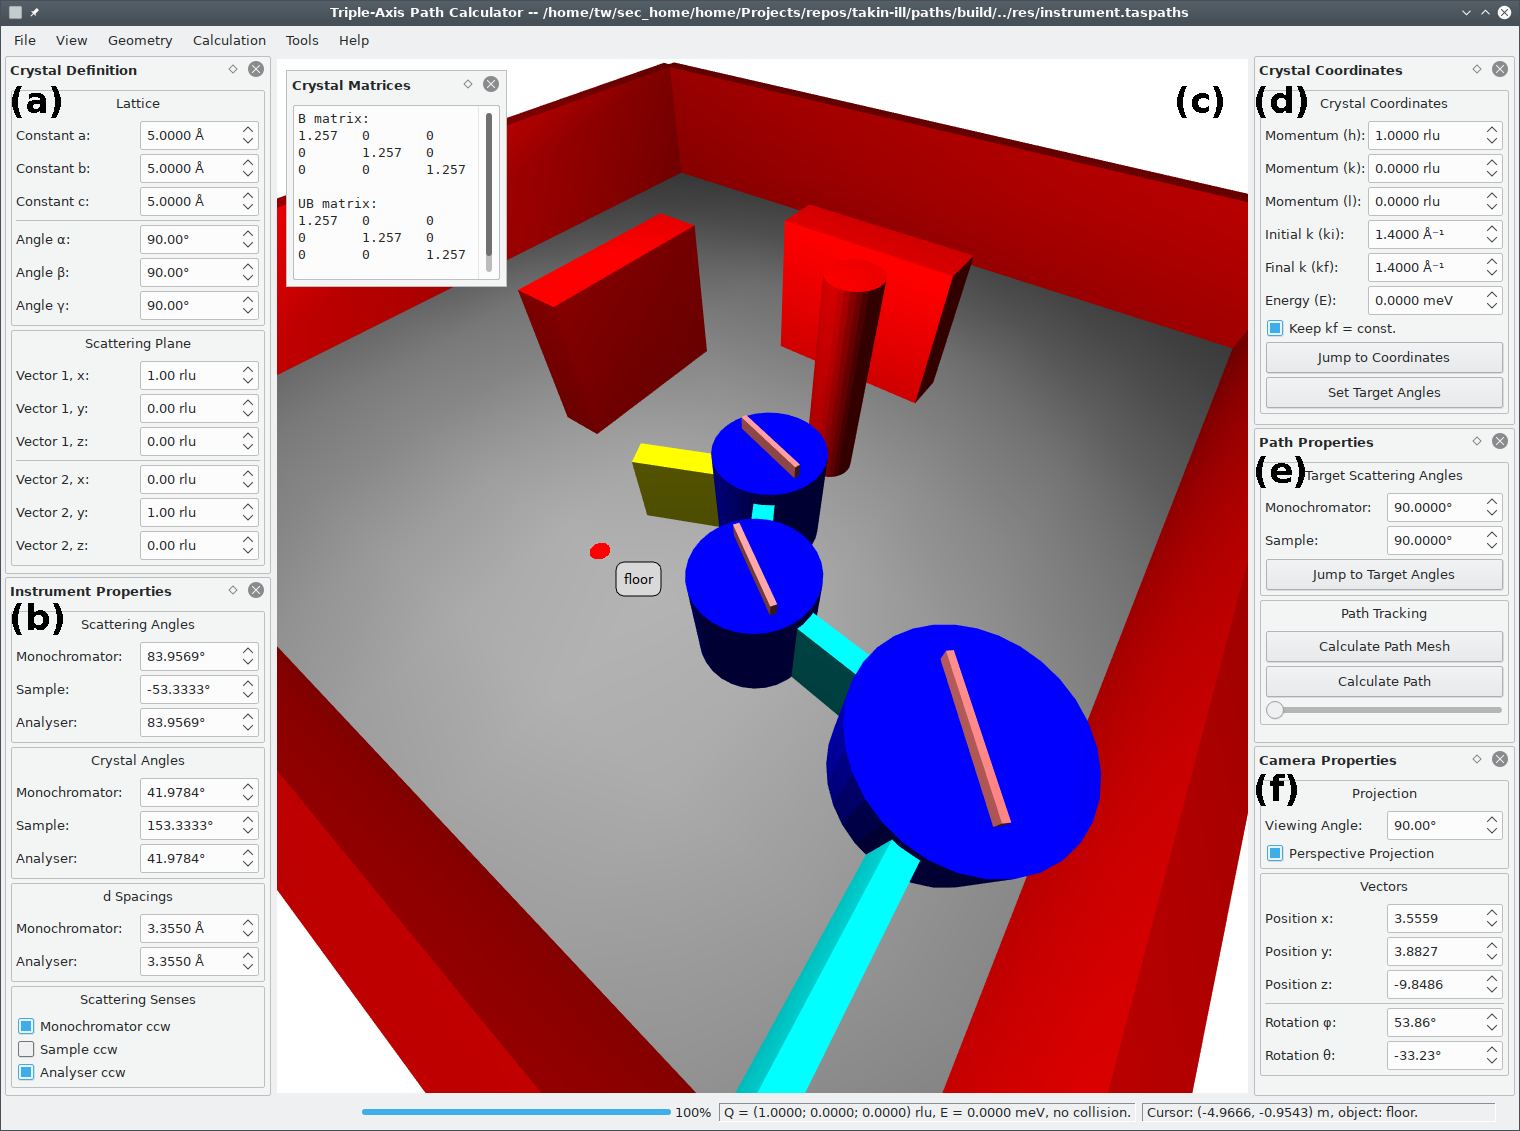
\includegraphics[width = 1 \textwidth]{figures/gui}
		\end{center}
	\caption[Main program GUI.]{Main GUI. 
		Here, instrument and sample crystal properties can be set up,
		walls can be added and moved. 
		Furthermore, paths around the walls can be calculated.
		The central view provides a three-dimensional visualisation of the instrument
		configuration and is fully dynamic: Each element, including the instrument
		and the wall segments, can be moved or manipulated using the mouse.
		See the text for a description of each interface element.
		\label{fig:gui}}
\end{figure}

The functions of the individual control elements of the main GUI, which are marked as (a)-(f)
in Fig. \ref{fig:gui}, are explained in the following sections. Each of the panels corresponds to a specific
functionality of the core module (chapter \ref{ch:impl}), to which all calculations are delegated. 
This way, the GUI is literally just an interface and only performs auxiliary calculations.
By the same token, the core module itself is completely independent of the GUI, or any other
interface code, and the full functionality of the software, except GUI-specific visualisation and editing
capabilities, is equally accessible from the other alternative interface modules, e.g. the \textit{Python}
interface described in section \ref{sec:scripting}, or the raw C++ library interface.

From within the GUI, the developer documentation is accessible via the ``Help'' menu.
The documentation for the entire source code is automatically generated using 
the \textit{Doxygen} \cite{web_doxygen} documentation generator.
Furthermore, a settings dialog exists which allows for a fine-tuning of the algorithm's
parameters.



\subsection{Crystal definition dock window}
\label{sec:gui_xtal}
\begin{minipage}{1 \textwidth}
\setlength{\intextsep}{0.25cm}
\begin{wrapfigure}{r}{0.46 \textwidth}
	\vspace{-0.25cm}
	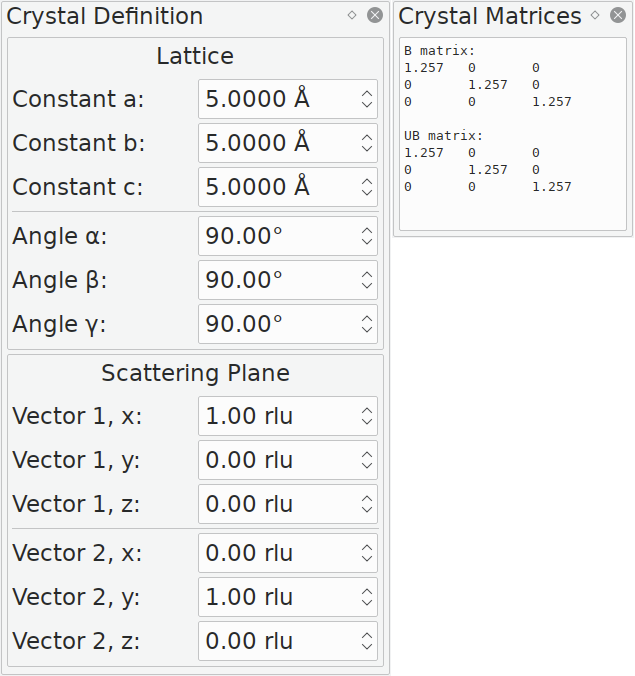
\includegraphics[width = 0.45 \textwidth]{figures/gui_xtal}
	\caption[Crystal definition window.]{Crystal definition window (a).
		\label{fig:gui_xtal}}
\end{wrapfigure}

Dock window (a) of the main GUI (Fig. \ref{fig:gui}) sets up the metric tensor \cite[pp. 807-809]{Arens2015}
corresponding to the crystal $UB$ matrix using the sample definition.
A magnified view of this window is provided in Fig. \ref{fig:gui_xtal}. 
As seen before, the $UB$ matrix transforms the crystal coordinate system into the instrument's 
laboratory coordinate system \cite{Lumsden2005}.
The necessary information for the $B$ matrix comprise the axis lengths of the sample lattice's
unit cell as well as the axis angles for the non-Cartesian crystal coordinate system.
The $UB$ matrix rotates the crystal coordinate system so that the $x$ and $y$ axes correspond
to the 2-d scattering plane accessible by the instrument.
The mathematical background to this formalism has been discussed in chapter \ref{ch:xtal}.
Finally, the $B$ and $UB$ matrices calculated from the entered crystal information are shown 
in the floating window right of (a).
\end{minipage}
\vspace{0.5cm}



\subsection{Instrument properties dock window}
\begin{minipage}{1 \textwidth}
\setlength{\intextsep}{0.25cm}
\begin{wrapfigure}{l}{0.3 \textwidth}
	\vspace{-0.25cm}
	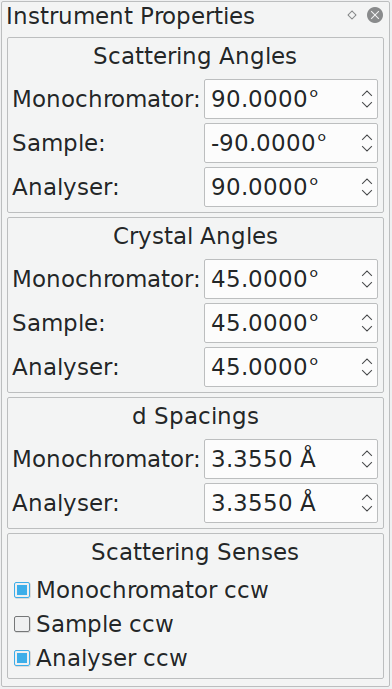
\includegraphics[width = 0.25 \textwidth]{figures/gui_instrument}
	\caption[Instrument properties window.]{Instrument properties window (b).
		\label{fig:gui_instr}}
\end{wrapfigure}

The raw instrument properties, which are agnostic of any sample crystal coordinates, are set up
using the dock window shown in Fig. \ref{fig:gui_instr}. It displays and lets the user modify
any crystal rotation angles, both the rocking angles of the crystals around their own axes
as well as the scattering angle with respect to the following axis. These angles and their
use in diffraction (two-axis) and spectroscopy (three-axis) instruments has been described 
in chapters \ref{ch:intro} and \ref{ch:xtal}. 
The fields named ``$d$ spacings'' correspond to the spacing of the crystal planes in the 
monochromator and analyser crystals. In our examples we use the value of $d\,=\,3.355\, \textup{\AA}$
which corresponds to scattering on the $\left(002\right)$ Bragg reflection of highly oriented
pyrolithic graphite (HOPG) \cite[p. 250]{Shirane2002}, which is one of the standard crystals used as a
monochromator or analyser in a TAS instrument.
Finally, the check boxes named ``scattering senses'' control the sign of the scattering angles.
If the box is checked, a positive angle corresponds to a counterclockwise sense, i.e. corresponding
to the usual mathematical definition, and alternatively to a clockwise sense when unchecked.
From the standpoint of the physics to be studied in the sample, these signs have no influence
in practice. They do, however, strongly affect the resolution of the instrument \cite{Eckold2014} \cite[p. 260]{Shirane2002}
and have to be considered carefully in the set-up of an experiment.
\end{minipage}



\subsection{Main workspace}
\label{sec:gui_gl}
The largest portion of the screen is reserved for the main workspace.
A typical view is shown in element (c) of Fig. \ref{fig:gui}.
Here, a graphical representation of the instrument space containing the instrument and the walls 
is performed using \textit{OpenGL} \cite{web_OpenGL} via \textit{Qt}'s
\lstinline[language=C++]|QOpenGLWidget| \cite{web_QOpenGLWidget} class.
The current view of the instrument is controlled by moving the mouse while holding the right button.
The camera position, viewing angle and direction as well as the type of projection matrix are 
displayed in dock window (f) and can also be entered directly.

The workspace is not restricted to a passive view of the instrument, but also functions as an editor
which allows for an easy interaction with the 3-d objects in the scene. For example, wall segments can
be inserted, edited and removed on the fly, see Fig. \ref{fig:gui_objects}.
The segments as well as the instrument axes themselves can be dynamically moved by dragging them using the 
mouse. This is realised by ``unprojecting'' the current mouse position from its coordinates with respect 
to the near and far planes of view frustum into the global object coordinate system in a first step, 
and finding all objects that intersect with a line through these two unprojected points in a second step. 
Mathematical details on this and other aspects of \textit{OpenGL} rendering have been discussed 
in chapter \ref{ch:gl}.
The renderer itself can be found in the class \lstinline[language=C++]|PathsRenderer|, located in
the file \lstinline|./src/gui/PathsRenderer.cpp|.

Internally, several data structures are maintained for the object system. 
The main hierarchical object system has its root in the \lstinline[language=C++]|InstrumentSpace|
class. This class is part of the core module (see chapter \ref{sec:tasmodel}) and is not dependent
on \textit{OpenGL} or the GUI.
To avoid introducing GUI- or rendering-specific details into the core, a second object
system is maintained in the GUI's \lstinline[language=C++]|PathsRenderer| itself. 
Here, all the \textit{OpenGL}-specific details, for example the vertex array objects \cite{wiki_vao} 
of all 3-d objects that are displayed on the screen, are stored.
Data in this secondary object system is updated automatically as soon as the user edits an object 
property from the main \lstinline[language=C++]|InstrumentSpace| instance.

\begin{figure}[htb]
	\begin{minipage}{0.45 \textwidth}
		\begin{center}
			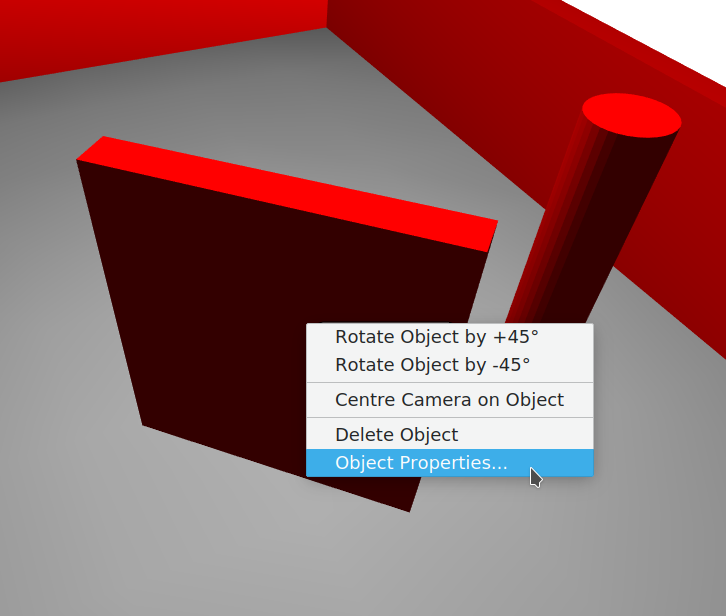
\includegraphics[width = 1 \textwidth]{figures/gui_object}
		\end{center}
	\end{minipage}
	\hspace{0.1cm}
	\begin{minipage}{0.5 \textwidth}
		\begin{center}
			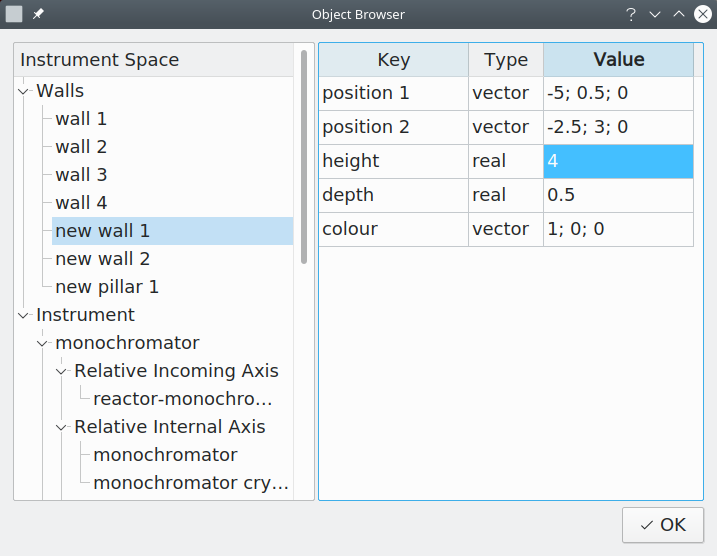
\includegraphics[width = 1 \textwidth]{figures/gui_objbrowser}
		\end{center}
	\end{minipage}
	\caption[Object manipulation.]{Manipulation of 3-d objects in the main GUI.
		Left panel: Objects can be moved by mouse and possess a context menu.
		Right panel: All objects in the instrument space are organised hierarchically. 
			Their properties can be dynamically edited, meaning that any change
			in the editor is immediately reflected in the \textit{OpenGL}
			visualisation, and vice versa.
		\label{fig:gui_objects}}
\end{figure}



\subsection{Crystal coordinates dock window}
\label{sec:gui_xtalcoords}
\begin{minipage}{1 \textwidth}
\setlength{\intextsep}{0.25cm}
\begin{wrapfigure}{r}{0.26 \textwidth}
	\vspace{-0.25cm}
	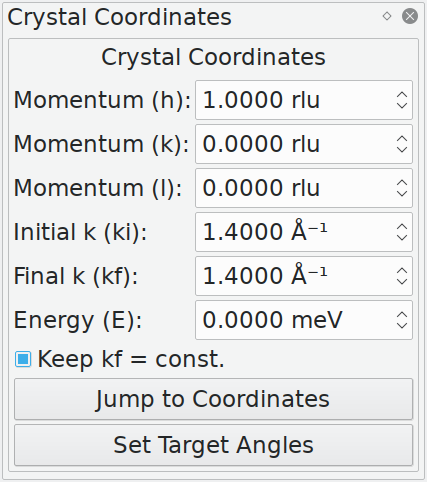
\includegraphics[width = 0.25 \textwidth]{figures/gui_xtalcoords}
	\caption[Crystal coordinates window.]{Crystal coordinates window (d).
		\label{fig:gui_xtalcoords}}
\end{wrapfigure}

Using the $UB$ transformation matrix that has been set up before (chapter \ref{sec:gui_xtal}),
an instrument position can be entered in the crystal coordinates dock window, which is
shown in Fig. \ref{fig:gui_xtalcoords}.
At triple-axis spectrometers, coordinates are given as four-dimensional tuples of the
form $\left(h\  k\  l\  E \right)^t$, where the three-dimensional momentum transfer
vector in the coordinate system of the instrument and its relation to the initial and final
wavevectors $\underline{k}_i$ and $\underline{k}_f$, is thus \cite[p. 11]{Shirane2002} \cite{Lumsden2005}
\begin{equation}
	\underline{Q}\ =\ UB\cdot \left(\begin{array}{c} h \\ k \\ l \end{array}\right) \ \equiv\ \underline{k}_i - \underline{k}_f.
\end{equation}
The fourth coordinate component, namely the energy transferred to the crystal, is \cite[p. 11]{Shirane2002}
\begin{equation}
	E \ =\ \frac{\left( \hbar k_i \right)^2}{2 m_n} - \frac{\left( \hbar k_f \right)^2}{2 m_n}.
\end{equation}
The checkbox labelled ``keep $k_f$ = const'' selects which one of the two wavenumbers, the incoming ($k_i$) 
or the outgoing ($k_f$), is kept constant and which is variable to effectuate the energy transfer
from the neutron to the sample.
Depending on the selected mode, the configuration space and motion planning calculations will either involve
the monochromator scattering angle (in case $k_f$ chosen to be constant), or the analyser scattering
angle (in case $k_i$ is chosen to be constant).
Please refer to chapters \ref{ch:intro} and \ref{ch:xtal} for details on the calculations and physical background.

The button labelled ``jump to coordinates'' sets the current (and initial path position)
of the instrument to the given crystal coordinates, whereas the ``set target angles'' button
sets the target position on the instrument path.

\end{minipage}



\subsection{Path properties dock window and dialog}
\begin{minipage}{1 \textwidth}
\setlength{\intextsep}{0.25cm}
\begin{wrapfigure}{l}{0.26 \textwidth}
	\vspace{-0.25cm}
	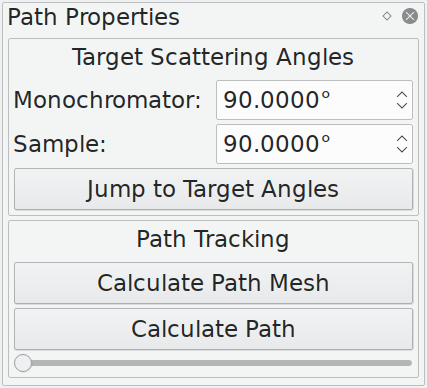
\includegraphics[width = 0.25 \textwidth]{figures/gui_path}
	\caption[Path properties window.]{Path properties window (e).
		\label{fig:gui_path}}
\end{wrapfigure}

Finally, the calculation of the instrument path is done using the path properties dock window
given in Fig. \ref{fig:gui_path}. Here, the target scattering angles are calculated from the crystal
coordinates and set by the previous step (section \ref{sec:gui_xtalcoords}). For direct positioning,
the angles can also be entered manually, thereby overriding the crystal coordinate calculations.

The button labelled ``calculate path mesh'' starts the calculation of the skeletal bisectors that are
described in chapter \ref{sec:polygonal_voronoi_diagram}.
Once a path mesh is available, the ``calculate path'' button finds the optimal path on the mesh and 
invokes the core library functions described in chapter \ref{sec:exepath}.
As soon as a path has been calculated, its positions can be tracked using the progress bar at the bottom
of the dock window.

Details on the path calculations, including the path mesh, are displayed in the angular configuration
space dialog that is depicted in Fig. \ref{fig:gui_configspace}.
Here, the start and target positions can also be directly dragged and dropped via mouse and the
effects on the calculation are visualised live.
The library \textit{QCustomPlot} \cite{web_QCustomPlot} is used for plotting.

\end{minipage}



\begin{figure}[htb]
		\begin{center}
			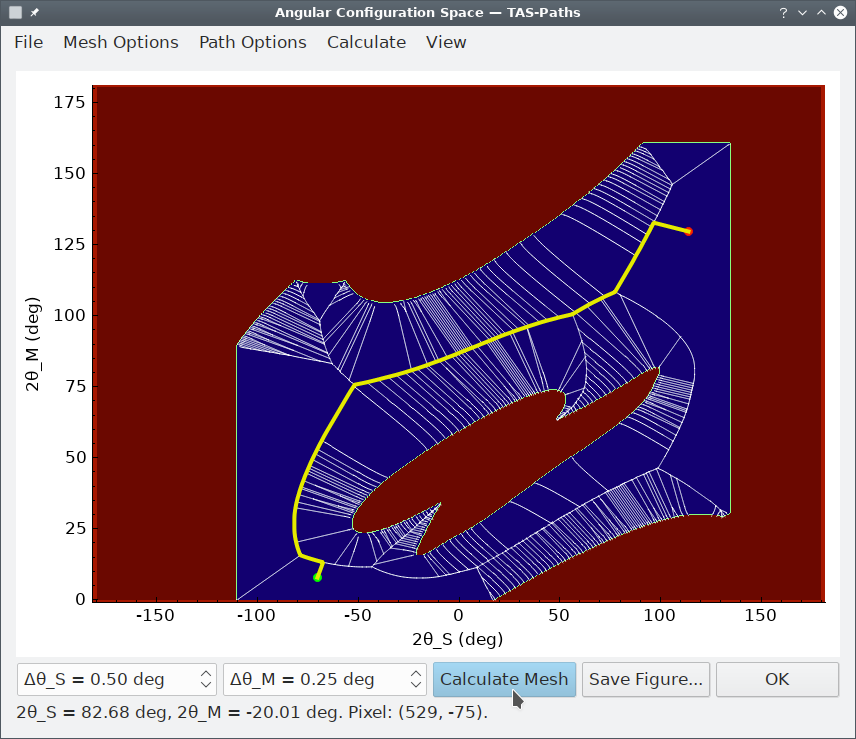
\includegraphics[width = 0.75 \textwidth]{figures/gui_configspace}
		\end{center}
	\caption[Configuration space dialog.]{Angular configuration space and path calculation dialog.
	Using the \textit{QCustomPlot} library \cite{web_QCustomPlot}, the dialog plots all possible
	instrument positions for the monochromator and sample scattering angles, $2\theta_M$ and $2\theta_S$, respectively.
	Forbidden positions are shown in red.
	These can be invalid angles as well as collisions of the instrument with walls
	(here, specifically, the pillar from Fig \ref{fig:gui}), or with itself.
	Allowed positions are drawn in blue. The mesh of all possible instrument
	paths is shown as white lines, while a currently selected example path from
	the red start to the green target position is shown as a yellow line.
		\label{fig:gui_configspace}}
\end{figure}


\subsection{Case study and illustrative example}
We proceed to present an illustrative example modelled after a situation that arose during an 
experiment that we performed at the instrument \textit{Thales} \cite{thales} some time ago. 
The situation is an archetypal one which often arises during a measurement and which
can be automatised and visualised using the present software.
The software was not yet available at the time of the experiment, though, so we still had to resort 
to long-winded manual driving of the instrument.

\paragraph{Problem}
After a series of scans, the instrument reached a position of 
$Q_\mathrm{start}\,=\,\left(1.5,\ 1.5,\ 0.5\right)\, \mathrm{rlu}$ and  $E_\mathrm{start}\,=\,10\, \mathrm{meV}$, where
$Q$ and $E$ refer to the momentum and energy transfer from the neutron to the crystal, respectively.
Here, ``rlu'' stands for \textit{relative lattice units}, see chapter \ref{ch:xtal}, and ``meV'' means energy units of milli-electronvolts,
which corresponds to the thousandths part of the energy gained by an electron moving through a potential of one volt \cite{wiki_eV}.
The real-space position of the instrument corresponding to these crystal coordinates is depicted in Fig. \ref{fig:casestudy_start}.
The crystal in question was cubic and had the lattice constant of $a = 8.9\,\textup{\AA}$, it was
oriented in a $(hhl)$ scattering plane, meaning that the plane was spanned by the vectors
$\left[1,\, 1,\, 0\right]$ and $\left[0,\, 0,\, 1\right]$.

For the next scans, the instrument was to drive back to the $\left(220\right)$ Bragg peak, 
i.e. to the coordinates $Q_\mathrm{target}\,=\,\left(2,\ 2,\ 0\right)\, \mathrm{rlu}$ and  $E_\mathrm{target}\,=\,0\, \mathrm{meV}$,
whose corresponding instrument configuration is depicted in Fig. \ref{fig:casestudy_target}.
Naively, one might assume that it were safe to directly drive the instrument from $\left(Q_\mathrm{start},\, E_\mathrm{start}\right)$
to $\left(Q_\mathrm{target},\, E_\mathrm{target}\right)$, as at least these two limiting positions are safe and nothing seems to block
the intermediate positions.

The control software would drive all motors at the same time, and the problem lies in the fact that not all motors
drive equally fast. The monochromator motors, which are responsible for selecting the energy transfer $E$, are
much slower than the two sample motors which drive the momentum transfer $Q$. In practice this would lead to
the situation where $Q$ has already reached the target position, while $E$ is still near its starting point, i.e. the instrument
would be at a mixed coordinate $\left(Q_\mathrm{target},\, E_\mathrm{start}\right)$,
which is shown in Fig. \ref{fig:casestudy_collision}.
As can be seen, issuing such a drive command would lead to a collision of the analyser drum with the outer wall.

\begin{figure}[H]
		\begin{center}
			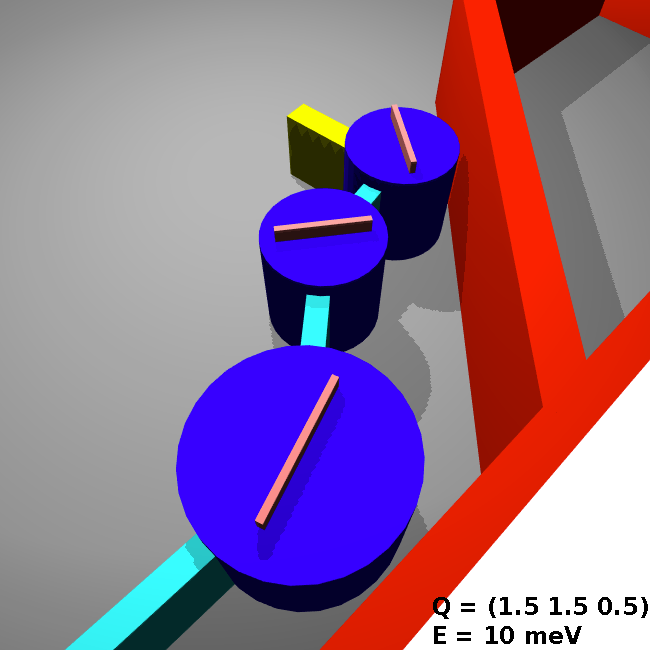
\includegraphics[width = 0.4 \textwidth]{figures/casestudy_15_15_05_10meV}
			\hspace{0.5cm}
			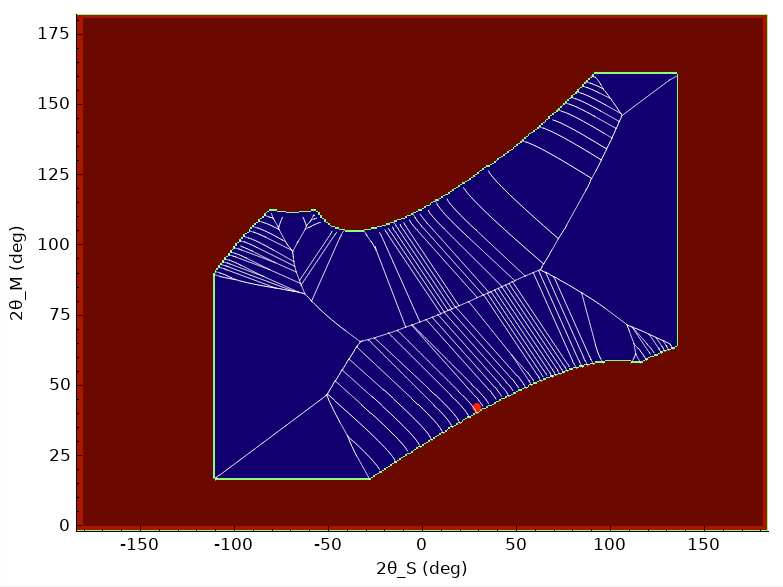
\includegraphics[width = 0.55 \textwidth]{figures/casestudy_15_15_05_10meV_cfg}
		\end{center}
	\caption[Case study: Start position.]{Start position shown in real (left) and in angular configuration space (right), 
		where the red dot indicates the current instrument position. 
		After some measurement the instrument was at a position
		corresponding to the crystal coordinates $Q_\mathrm{start}\,=\,\left(1.5,\ 1.5,\ 0.5\right)\, \mathrm{rlu}$ and 
		energy transfer $E_\mathrm{start}\,=\,10\, \mathrm{meV}$.
		\label{fig:casestudy_start}}
\end{figure}

\begin{figure}[H]
		\begin{center}
			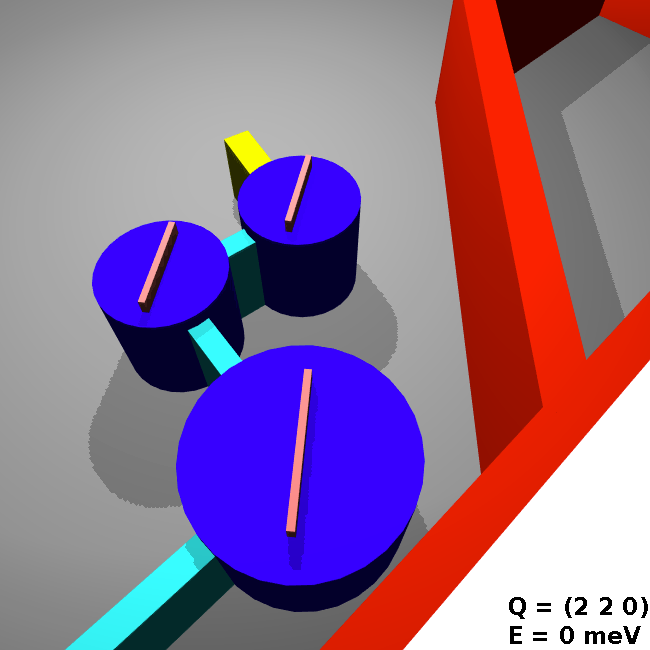
\includegraphics[width = 0.4 \textwidth]{figures/casestudy_2_2_0_0meV}
			\hspace{0.5cm}
			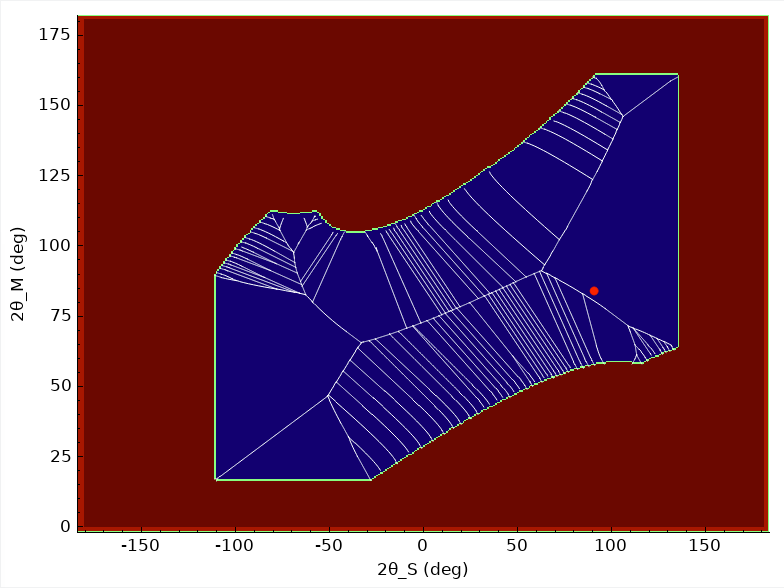
\includegraphics[width = 0.55 \textwidth]{figures/casestudy_2_2_0_0meV_cfg}
		\end{center}
	\caption[Case study: Target position.]{Target position shown in real (left) and in angular configuration space (right). 
		The next set of measurements required the instrument
		to move to the crystal coordinates $Q_\mathrm{target}\,=\,\left(2,\ 2,\ 0\right)\, \mathrm{rlu}$ and 
		energy transfer $E_\mathrm{target}\,=\,0\, \mathrm{meV}$.
		\label{fig:casestudy_target}}
\end{figure}

\begin{figure}[H]
		\begin{center}
			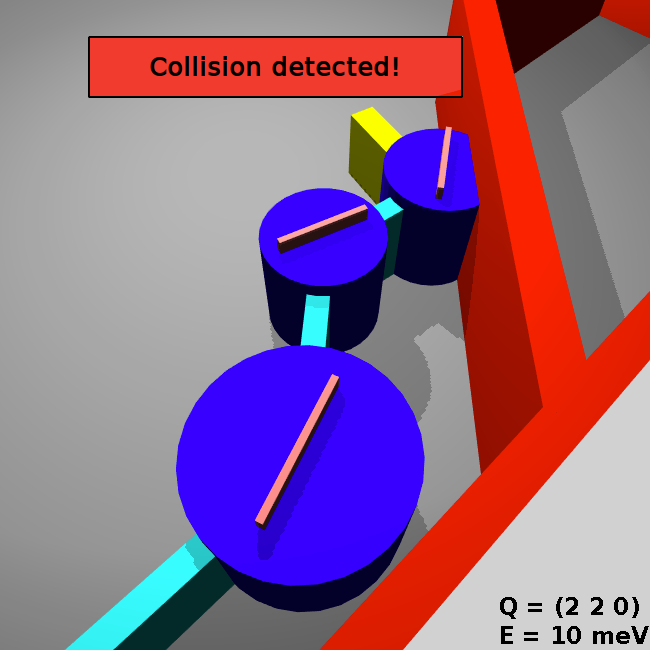
\includegraphics[width = 0.4 \textwidth]{figures/casestudy_2_2_0_10meV}
			\hspace{0.5cm}
			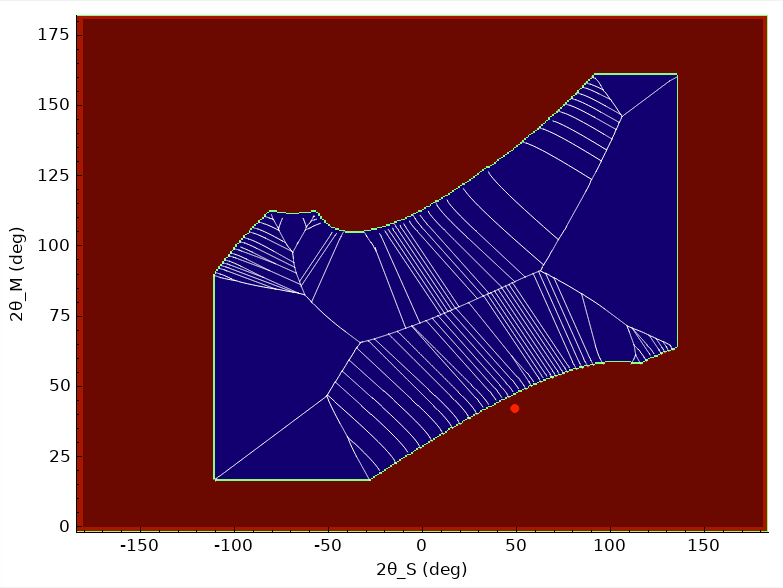
\includegraphics[width = 0.55 \textwidth]{figures/casestudy_2_2_0_10meV_cfg}
		\end{center}
	\caption[Case study: Collision.]{Collision. 
		If one were to drive the instrument directly from $\left(Q_\mathrm{start},\, E_\mathrm{start}\right)$ (Fig. \ref{fig:casestudy_start})
		to $\left(Q_\mathrm{target},\, E_\mathrm{target}\right)$ (Fig. \ref{fig:casestudy_target}), the instrument 
		would collide with the outer wall due to the monochromator motors being much slower than the other 
		motors of the instrument (see text for more explanations).
		\label{fig:casestudy_collision}}
\end{figure}



\paragraph{Solution}
The problem of avoiding the collision with the outer wall  is easily solved by calculating the
path along the skeleton mesh using the software. Figures \ref{fig:casestudy_sequence1} and 
\ref{fig:casestudy_sequence2} show key frames of the driving sequence from the start to the 
target position.
As can be seen in the figure panels, the algorithm ensures that first the monochromator 
(related to the energy) is driven primarily, while the sample scattering angle (related to the momentum) 
is initially driven away from the wall and in the opposite direction than that of its final position (Steps 1-3
in the panels of Fig. \ref{fig:casestudy_sequence1}).
The second part of the sequence primarily drives the sample scattering angle to nearly its
envisaged end position while also still continuing to drive the monochromator (Steps 3-4
in Figures \ref{fig:casestudy_sequence1} and \ref{fig:casestudy_sequence2}).
The third and final part continued driving the sample scattering angle, but drives the monochromator
back a bit, until both reach their target position (Steps 4-5 in Fig. \ref{fig:casestudy_sequence2}).

\begin{figure}[htb]
		\begin{center}
			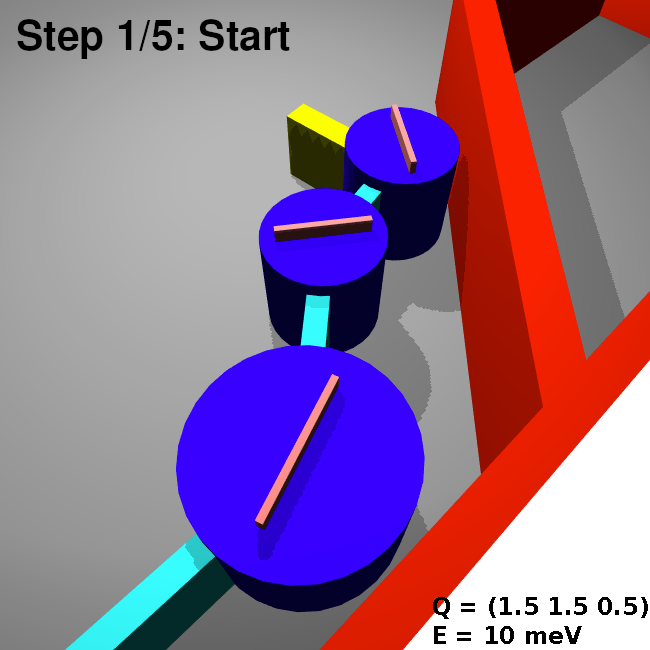
\includegraphics[width = 0.4 \textwidth]{figures/casestudy_step0}
			\hspace{0.5cm}
			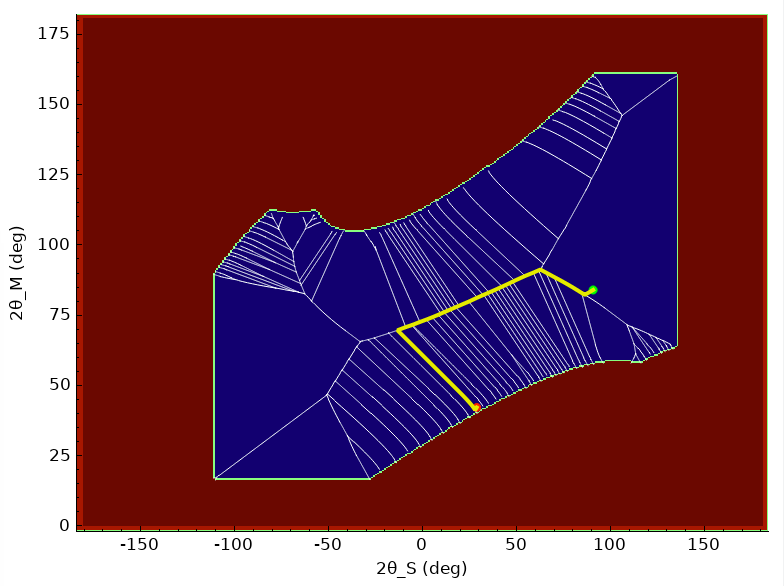
\includegraphics[width = 0.55 \textwidth]{figures/casestudy_path}
			\vspace{0.2cm}
			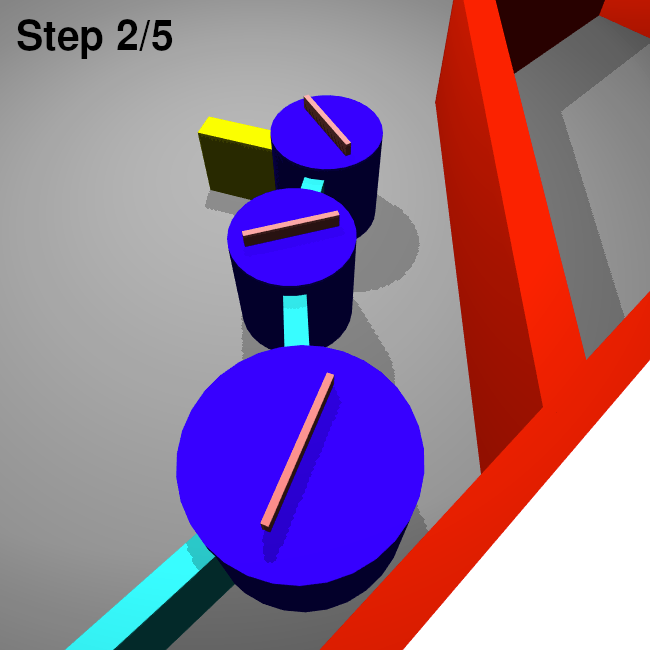
\includegraphics[width = 0.4 \textwidth]{figures/casestudy_step1}
			\hspace{0.5cm}
			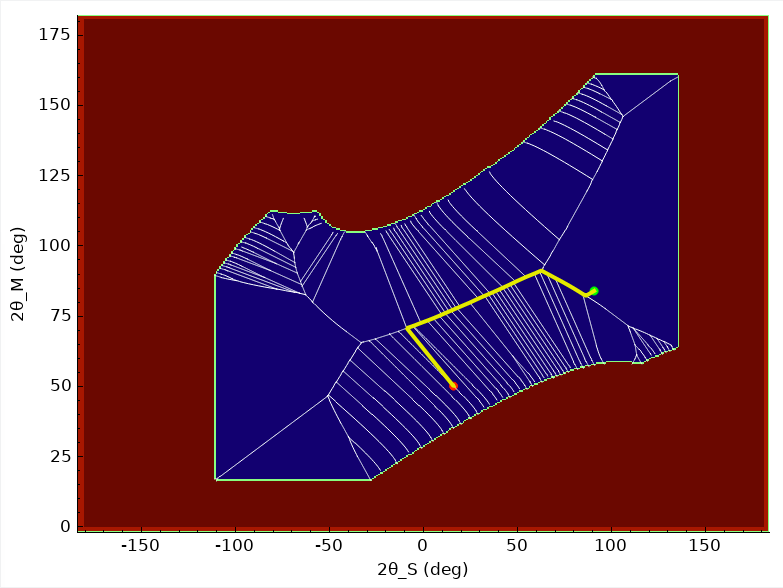
\includegraphics[width = 0.55 \textwidth]{figures/casestudy_step1_cfg}
			\vspace{0.2cm}
			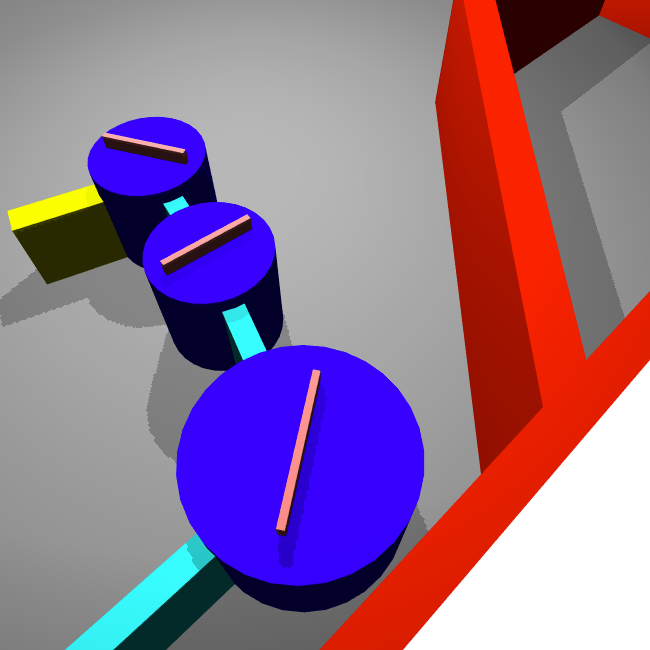
\includegraphics[width = 0.4 \textwidth]{figures/casestudy_step2}
			\hspace{0.5cm}
			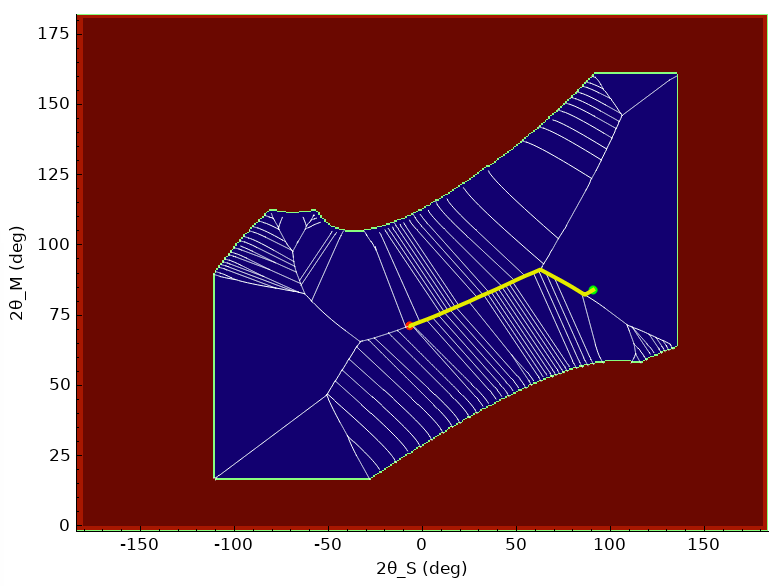
\includegraphics[width = 0.55 \textwidth]{figures/casestudy_step2_cfg}
		\end{center}
	\caption[Case study: Path 1/2.]{The first three steps of the path leading from the start
		to the target position and avoiding the collision with the outer wall. As before, the
		left-hand sides show the real-space instrumental configuration, while the right-hand
		sides show the corresponding angular configuration space with the red dot indicating the
		current instrument position, and the green dot being the target position.
		The calculated optimal path is drawn as a yellow line.
		\label{fig:casestudy_sequence1}}
\end{figure}

\begin{figure}[htb]
		\begin{center}
			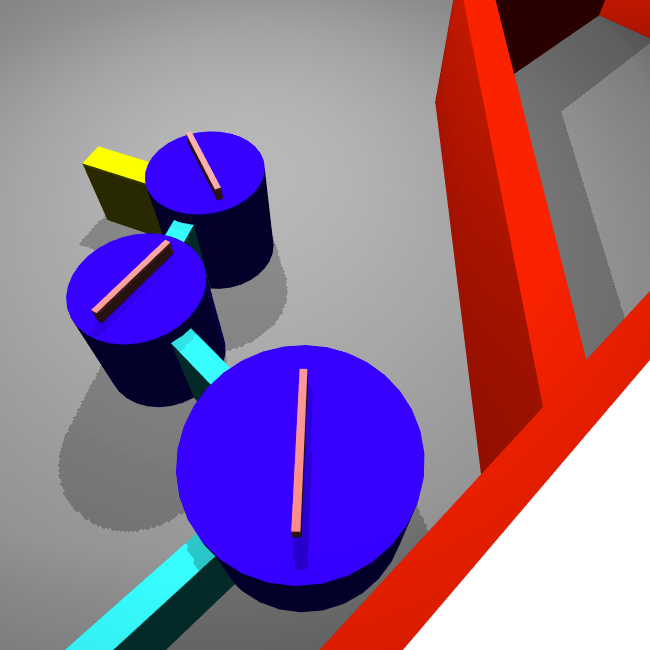
\includegraphics[width = 0.4 \textwidth]{figures/casestudy_step3}
			\hspace{0.5cm}
			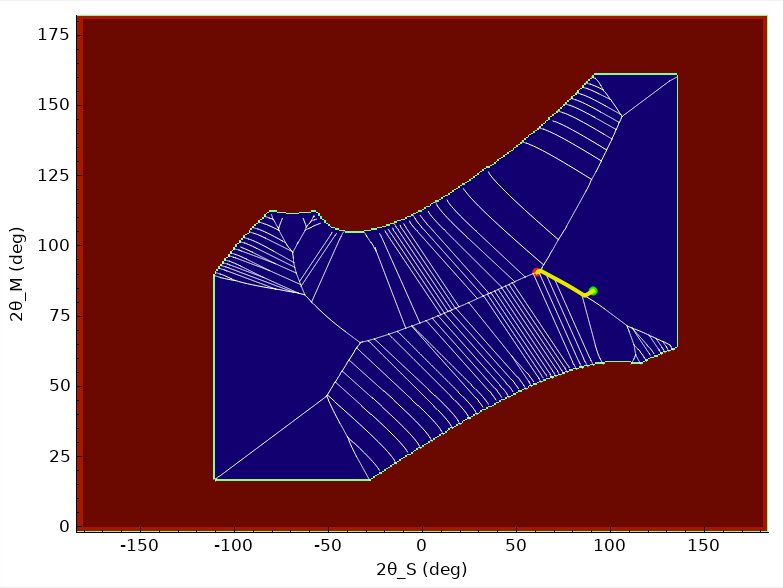
\includegraphics[width = 0.55 \textwidth]{figures/casestudy_step3_cfg}
			\vspace{0.2cm}
			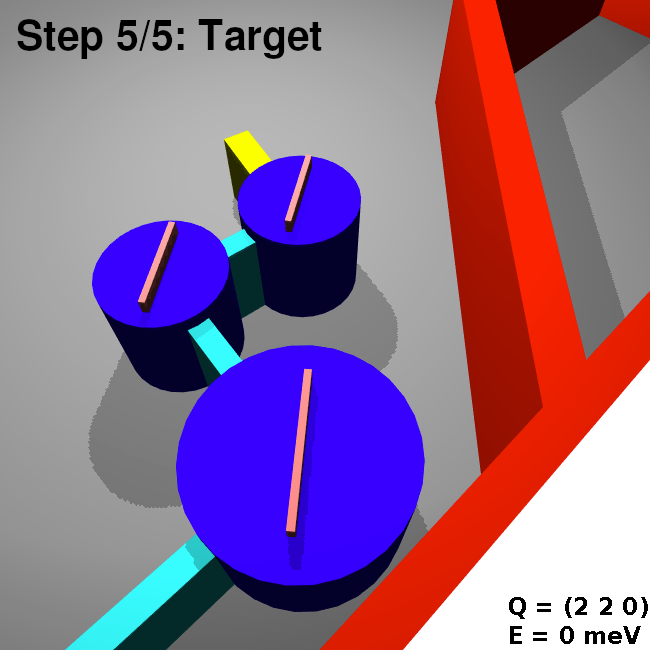
\includegraphics[width = 0.4 \textwidth]{figures/casestudy_step4}
			\hspace{0.5cm}
			\includegraphics[width = 0.55 \textwidth]{figures/casestudy_2_2_0_0meV_cfg}
		\end{center}
	\caption[Case study: Path 2/2.]{The second two steps of the path leading from the start
		to the target position and avoiding the collision with the outer wall.
		The left-hand sides show the real-space instrumental configuration, while the right-hand
		sides show the corresponding angular configuration space with the red dot indicating the
		current instrument position, and the green dot being the target position.
		The calculated optimal path is drawn as a yellow line.
		\label{fig:casestudy_sequence2}}
\end{figure}



\section{Python scripting interface}
\label{sec:scripting}

In order to allow for a simple way to automatise recurring calculations and workflows, as well as to provide
a possibility for inclusion of the core module (see section \ref{sec:library}) of the present 
software in other tools, a scripting interface has been developed using the interface generator \textit{SWIG} \cite{web_swig}. 
\textit{SWIG} is a tool which parses C or C++ header files and creates a native interface 
for several possible scripting languages, of which we opted for \textit{Python} \cite{Rossum2011, web_python} 
as it has become one of the most popular programming language in neutron science over the last decade.
As the core module already has the structure of a library, the effort to offer scripting functionality
was minimal. Only a few helper functions had to be included in several classes, because \textit{SWIG}
is not yet fully C++20 compliant and had some problems with new language features such as 
template concepts \cite{cppwiki_concepts}.
The \textit{SWIG} interface definition, which maps the C++ classes to corresponding \textit{Python} 
classes of the same name, can be found in the file \lstinline|./scripting/taspaths.i| of the source repository.

\paragraph{Typical workflow}
An example of the full workflow consisting of loading an instrument definition file, creating a path 
mesh and finding the path from a start position in crystal coordinates to a target position is given in listings 
\ref{lst:pyworkflow1}, \ref{lst:pyworkflow2} and \ref{lst:pyworkflow3}.
The native core module is imported into \textit{Python} as the name \lstinline[language=C++]|tas| on line 9 of the script,
instances of its classes are generated for the individual functionalities.
Specifically, the instrument space class from chapter \ref{sec:tasmodel}, which is the representation of the instrument 
and which is furthermore responsible for the local instrument axis coordinate systems, collision detection, as well as 
loading and saving of instrument configurations, is created on line 37. 
Next, the triple-axis and single-crystal calculator class from chapter \ref{ch:xtal} is created on line 51 and is 
used to set-up the instrument scattering senses and a single-crystal coordinate system.
Finally, the path builder class, which has been described in chapter \ref{sec:buildpath}, is created on line 64 
and used in the rest of the script to calculate the path mesh as well as the concrete path between the 
given crystal coordinate points.
The results of the script are shown in Fig. \ref{fig:pyworkflow}, where we employ \textit{Matplotlib} 
\cite{Hunter2007, web_matplotlib} to plot the calculated path and the obstacles in configuration space.

\begin{figure}[htb]
		\begin{center}
			\includegraphics[width = 0.66 \textwidth]{figures/pyworkflow}
		\end{center}
	\caption[Python workflow results.]{Results from the \textit{Python} workflow example of listings
		\ref{lst:pyworkflow1}, \ref{lst:pyworkflow2} and \ref{lst:pyworkflow3}, directly plotted 
		in \textit{Python} using \textit{Matplotlib} \cite{Hunter2007, web_matplotlib}.
		The obstacles are shown as red regions, the calculated instrument path is shown as a blue curve.
		\label{fig:pyworkflow}}
\end{figure}


\begin{listing}[htb]
	\begin{lstlisting} [language = Python, 
		basicstyle = {\scriptsize},
		breaklines = true, tabsize = 4,
		numbers = left, firstnumber = 1, numberstyle={\scriptsize}]
import sys
import os
import math as m

cwd = os.getcwd()
sys.path.append(cwd)

# import native C++ core module
import taspaths as tas

# -----------------------------------------------------------------------------
# helper functions
# -----------------------------------------------------------------------------
def error(msg):
	print("Error: %s" % msg)
	exit(-1)

def warning(msg):
	print("Warning: %s" % msg)
# -----------------------------------------------------------------------------

# -----------------------------------------------------------------------------
# options
# -----------------------------------------------------------------------------
write_pathmesh = False
write_path = False
show_plot = True
file_name = "../res/instrument.taspaths"
# -----------------------------------------------------------------------------

# -----------------------------------------------------------------------------
# load instrument
# -----------------------------------------------------------------------------
print("Loading instrument definition...")

# create the instrument space and load an instrument definition
instrspace = tas.InstrumentSpace()
[file_ok, file_date] = tas.InstrumentSpace.load(file_name, instrspace)

if file_ok:
	print("Loaded \"%s\", dated %s." % (file_name, file_date))
else:
	error("Could not load \"%s\"." % (file_name))

print("Instrument definition loaded.\n")
# -----------------------------------------------------------------------------

# -----------------------------------------------------------------------------
# set-up a sample single-crystal
# -----------------------------------------------------------------------------
tascalc = tas.TasCalculator()
tascalc.SetScatteringSenses(True, False, True)
tascalc.SetSampleLatticeConstants(5, 5, 5)
tascalc.SetSampleLatticeAngles(90, 90, 90, True)
tascalc.UpdateB()
tascalc.UpdateUB()
# -----------------------------------------------------------------------------
	\end{lstlisting}
	\caption[Python workflow example 1/3.]{Script showing an example workflow in \textit{Python}.
	Part 1 of 3: Set-up of the instrument and the sample crystal.
	\label{lst:pyworkflow1}}
\end{listing}



\begin{listing}[htb]
	\begin{lstlisting} [language = Python, 
		basicstyle = {\scriptsize},
		breaklines = true, tabsize = 4,
		numbers = left, firstnumber = 58, numberstyle={\scriptsize}]
# -----------------------------------------------------------------------------
# build path mesh
# -----------------------------------------------------------------------------
print("Building path mesh...")

# create the paths builder object
builder = tas.PathsBuilder()
builder.AddConsoleProgressHandler()
builder.SetInstrumentSpace(instrspace)
builder.SetTasCalculator(tascalc)
print("Path builder uses %d threads." % builder.GetMaxNumThreads())

# angular ranges to probe
angle_padding = 4.
a2_delta = 1./180.*m.pi
a4_delta = 2./180.*m.pi
a2_begin = 0. - angle_padding*a2_delta
a2_end = m.pi + angle_padding*a2_delta
a4_begin = -m.pi - angle_padding*a4_delta
a4_end = m.pi + angle_padding*a4_delta

if not builder.CalculateConfigSpace(
	a2_delta, a4_delta,
	a2_begin, a2_end,
	a4_begin, a4_end):
	error("Angular configuration space could not be calculated.")

if not builder.CalculateWallContours(True, False):
	error("Obstacle contours could not be calculated.")

if not builder.CalculateLineSegments():
	error("Line segments could not be calculated.")

if not builder.CalculateVoronoi(False):
	error("Voronoi diagram could not be calculated.")

print("Finished building path mesh.\n")
# -----------------------------------------------------------------------------

# -----------------------------------------------------------------------------
# set-up the start and target coordinates of a path
# -----------------------------------------------------------------------------
print("Calculating path...")

tascalc.SetKf(1.4)
start_angles = tascalc.GetAngles(0.5, 0., 0., 1.)
target_angles = tascalc.GetAngles(1.5, -0.5, 0., 2.5)

# take absolute angles
start_angles.monoXtalAngle = abs(start_angles.monoXtalAngle)
start_angles.sampleXtalAngle = abs(start_angles.sampleXtalAngle)
start_angles.sampleScatteringAngle = abs(start_angles.sampleScatteringAngle)
target_angles.monoXtalAngle = abs(target_angles.monoXtalAngle)
target_angles.sampleXtalAngle = abs(target_angles.sampleXtalAngle)
target_angles.sampleScatteringAngle = abs(target_angles.sampleScatteringAngle)

print("Start angles: a1 = %.2f deg, a5 = %.2f deg, a3 = %.2f deg, a4 = %.2f deg." % (
	start_angles.monoXtalAngle / m.pi*180.,
	start_angles.anaXtalAngle / m.pi*180.,
	start_angles.sampleXtalAngle / m.pi*180.,
	start_angles.sampleScatteringAngle / m.pi*180.))

print("Target angles: a1 = %.2f deg, a5 = %.2f deg, a3 = %.2f deg, a4 = %.2f deg." % (
	target_angles.monoXtalAngle / m.pi*180.,
	target_angles.anaXtalAngle / m.pi*180.,
	target_angles.sampleXtalAngle / m.pi*180.,
	target_angles.sampleScatteringAngle / m.pi*180.))
# -----------------------------------------------------------------------------
	\end{lstlisting}
	\caption[Python workflow example 2/3.]{Script showing an example workflow in \textit{Python}.
	Part 2 of 3: Calculation of the path mesh and the start and target positions from their crystal coordinates.
	\label{lst:pyworkflow2}}
\end{listing}


\begin{listing}[htb]
	\begin{lstlisting} [language = Python, 
		basicstyle = {\scriptsize},
		breaklines = true, tabsize = 4,
		numbers = left, firstnumber = 126, numberstyle={\scriptsize}]
# -----------------------------------------------------------------------------
# find path
# -----------------------------------------------------------------------------
path = builder.FindPath(
		start_angles.monoXtalAngle * 2., start_angles.sampleScatteringAngle,
		target_angles.monoXtalAngle * 2., target_angles.sampleScatteringAngle)
if not path.ok:
	error("No path could be found.")

builder.SetSubdivisionLength(0.5)
vertices = builder.GetPathVerticesAsPairs(path, True, True)

print("Finished calculating path.\n")
# -----------------------------------------------------------------------------

# -----------------------------------------------------------------------------
# output and plotting
# -----------------------------------------------------------------------------
# write the path mesh vertices to a file
if write_pathmesh:
	if not builder.SaveToLinesTool("lines.xml"):
		warning("Could not save line segment diagram.")

# write the path vertices to a file
if write_path:
	with open("path.dat", "w") as datafile:
		for vertex in vertices:
			datafile.write("%.4f %.4f\n" % (vertex[0], vertex[1]))

# plot the angular configuration space
if show_plot:
	import matplotlib.pyplot as plt

	# plot obstacles
	numgroups = builder.GetNumberOfLineSegmentRegions()
	print("Number of regions: %d." % numgroups)
	for regionidx in range(numgroups):
		region = builder.GetLineSegmentRegionAsArray(regionidx)
		x1, y1, x2, y2 = zip(*region)
		plt.fill(x1, y1, "-", linewidth = 1,
			fill = not builder.IsRegionInverted(regionidx), 
			color = "#ff0000")

	# plot path
	x, y = zip(*vertices)
	plt.xlabel("Sample Scattering Angle 2\u03b8_S (deg)")
	plt.ylabel("Monochromator Scattering Angle 2\u03b8_M (deg)")
	plt.plot(x, y, "-", linewidth=2)

	plt.show()
# -----------------------------------------------------------------------------

	\end{lstlisting}
	\caption[Python workflow example 3/3.]{Script showing an example workflow in \textit{Python}.
	Part 3 of 3: Calculation of the path between the start end target positions and plotting.
	\label{lst:pyworkflow3}}
\end{listing}


\section{Summary}
The modular design of the software keeps the interface code separate from the calculation core.
Several different types of interfaces were discussed in this chapter, most prominently the graphical 
user interface, which provides the most accessible way for the end user to interact with the software.
We demonstrated a typical situation of the instrument colliding with an outer wall, which arose 
during one of our past measurements, and which can be solved graphically using the software's GUI.
A separate scripting interface makes it easy to automatise calculations on the command line and 
to interface with other software tools.

Having outlined the entirety of the software, what remains to be done in the next chapter
is a description of the tools used to ensure that it stays bug-free, for example when
introducing new features to the core module.

%
% tests
% @author Tobias Weber <tweber@ill.fr>
% @date aug-2021
% @license see 'LICENSE' file
%

\chapter{Test Tools and Unit Tests}
\label{ch:tests}
Due to a rapid increase in its complexity over time, the software of this work 
necessitated a multi-tiered testing strategy during development, including test programs and unit tests.
Even after having finished the critical phases of development, the programs which are 
presented in this chapter serve to ensure that the software and its parts continue to work as intended. 
Problems that may arise can be rapidly analysed using the simplified environments these tools provide.

Before having being integrated into the main library or the GUI program, each essential function was tested 
separately. This was done either via small test programs or via dedicated unit tests, which are discussed in 
section \ref{sec:unit_tests}.
Integration tests of algorithms, where collections of functions are tested how and if they work together, 
were performed using larger bespoke test tools, which implemented a simplified versions of the functionality 
of the main programs. These are described in section \ref{sec:tests_tools}.



\section{Test tools}
\label{sec:tests_tools}
First, we describe the collection of tools that served in testing aspects of the main path-finding algorithm.
These tools share a common \textit{Qt}-based \cite{web_Qt} GUI codebase and are similar in their usage.
They all use the \lstinline[language=C++]|QGraphicsScene| class \cite{web_QGraphicsScene} and through that
allow a dynamic manipulation of their respective geometrical objects using the mouse. 
Calculations and results are automatically updated once the user changes the geometrical scenes.

Early versions of these tools were originally created in 2020 as preparation for the exam in the Algorithmic
Geometry course, the original repository can be found on-line at \url{https://github.com/t-weber/geo}. 
Afterwards, these programs were further developed for their current purpose during the present work.


\subsection{Line segments tool}
\label{sec:tests_linesegs}
The line segment tool (Fig. \ref{fig:linesgui}), whose code can be found in the file 
\lstinline|./src/tools/lines.cpp| of the source repository, 
performs several kinds of computations to test the line-based algorithms that are used in the core module.

The most important of these is the calculation of line segment Voronoi diagram bisectors as shown in 
Fig. \ref{fig:linesgui} (a), please also refer to chapter \ref{sec:voro_ls}.
To that end, it uses three different backend libraries between which the user can switch dynamically in
the program. These three backend libraries are \textit{Boost.Polygon}'s Voronoi module \cite{web_boost_polygon_voronoi},
the \textit{2D Segment Delaunay Graphs} \cite{web_2dsegdel} library, and \textit{OpenVoronoi} \cite{web_openvoronoi}.
The correctness of the calculation is furthermore checked by iterating the points of the $\mathbb{R}^2$ plane
on a grid and testing to which line segment they are closest. These are the coloured regions in Fig. \ref{fig:linesgui} (a).
The line segment tool can load the regions of the angular configuration space that are calculated in the main
program (chapter \ref{sec:line_seg_generation}), and was used for debugging purposes in its development and
for testing different approaches to the algorithms used in the main program.

Another calculation the line segment tool performs and which is shown in Fig. \ref{fig:linesgui} (b), is the 
calculation of trapezoidal maps (chapter \ref{sec:pointrobot_sector}), which are calculated according to the 
algorithm given in Ref. \cite[Ch. 6, pp. 121-146]{Berg2008}.
The purpose of this was for early testing which sector-based method would be most suitable
for path-mesh building. The trapezoid maps were deemed infeasible and were ruled out after
these tests.

The third calculation that was tested in this tool is the sweep-based intersection of line segments which
is used in the main algorithm for intersections checks between polygons, as has been discussed in 
chapter \ref{sec:angular_config_space}.
The implementation is based on the algorithm given in Ref. \cite[pp. 69-80]{FUH_geo2020}.

\begin{figure}[h]
	\centering
	\includegraphics[width = 0.49 \textwidth]{figures/linesgui_voro}
	\hspace{0.05cm}
	\includegraphics[width = 0.49 \textwidth]{figures/linesgui_trapezoid}

	\vspace{0.25cm}
	\includegraphics[width = 0.49 \textwidth]{figures/linesgui_inters}
	\caption[Line segments tool.]{Line segments tool.
		This program allows the dynamic calculation of
		(a) line segment Voronoi regions (coloured) and bisectors (black lines),
		(b) trapezoidal maps, and
		(c) sweep-based points of intersection (green points).
		Line segment vertices can be inserted, deleted and moved using the mouse.
		\label{fig:linesgui}}
\end{figure}



\subsection{Polygon tool}
The next tool performs calculations and tests on polygonal algorithms. 
Its source code can be found in the file \lstinline|./src/tools/poly.cpp|.

The main purpose of the polygon tool is the testing of the algorithm used for splitting concave 
polygonal regions into convex sub-regions that is used in building the path mesh in chapter \ref{sec:convex_regions}. 
Fig. \ref{fig:polygui} (a) shows a screenshot of a test run of the algorithm on a much simpler
polygonal region than what is calculated in the main program. The polygonal splitting algorithm 
itself is based on the description from Ref. \cite{Hegazy2014}.
Another function of the tool is the calculation of the visibility kernel \cite{TODO} of a 
polygonal region, see Fig. \ref{fig:polygui} (b).


\begin{figure}[h]
	\centering
	\includegraphics[width = 0.49 \textwidth]{figures/polygui_convex}
	\hspace{0.05cm}
	\includegraphics[width = 0.49 \textwidth]{figures/polygui_kernel}
	\caption[Polygon tool.]{Polygon tool.
		This program calculates the
		(a) convex sub-regions of a concave polygon, and
		(b) the visibility kernel (red) of a polygonal region.
		Polygon vertices can be inserted, deleted and moved using the mouse, updates
		are performed dynamically.
		\label{fig:polygui}}
\end{figure}



\subsection{Convex hull tool}
\label{sec:tests_hull}
The final tool performs calculations on collections of vertices.

Its main functionality consists of determining the convex hull \cite[Ch. 11, pp. 243-258]{Berg2008}, 
the Voronoi diagrams \cite[Ch. 7, pp. 147-171]{Berg2008}, 
as well as the Delaunay triangulation \cite[Ch. 9, pp. 191-218]{Berg2008} 
of the given set of vertices. This is shown in Fig. \ref{fig:hullgui} (a).
A secondary feature, depicted in Fig. \ref{fig:hullgui} (b), is the calculation of 
the minimal spanning tree between the vertices using Kruskal's algorithm \cite[pp. 265-268]{Erickson2019}.

For calculating the convex hull, several different algorithms have been implemented,
which can be selected in the program's ``backend'' menu.
These backends comprise the contour polygon method \cite[Ch. 3.1.5, pp. 125-128]{FUH_geo2020},
the iterative incremental calculation \cite[Ch. 3.1.3, pp. 117-123]{FUH_geo2020}, as well as the 
recursive divide-and-conquer method \cite[Ch. 3.1.4, pp. 123-125]{FUH_geo2020}, 
which have been implemented according to the pseudo-codes and descriptions given
in the respective references.
One further backend includes calculation via the \textit{QHull} library \cite{web_qhull}.
Not surprisingly, all backends yield the same results.

Similarly to the convex hull calculation, the calculation of the Delaunay triangulation
also supports multiple backend algorithms.
Among them are the incremental method \cite[Ch. 6.2, pp. 269-282]{FUH_geo2020}, 
delegating calculations \textit{QHull} \cite{web_qhull}, 
and third, the parabolic transformation \cite[Ch. 6.5, pp. 298-300]{FUH_geo2020}, 
which also partially uses \textit{QHull}, namely to calculate the three-dimensional 
convex hull of the transformed problem.

\begin{figure}[h]
	\centering
	\includegraphics[width = 0.49 \textwidth]{figures/hullgui_voro}
	\hspace{0.05cm}
	\includegraphics[width = 0.49 \textwidth]{figures/hullgui_kruskal}
	\caption[Convex hull tool.]{Convex hull tool.
		This program calculates 
		(a) the convex hull (thick black lines), the Voronoi diagram (red lines), 
			the Delaunay triangulation (thin black lines), as well as
		(b) Kruskal's minimum spanning tree (green lines)
		of a collection of vertices.
		As with the other test tools, the vertices can be inserted, deleted and moved 
		using the mouse, updates are performed dynamically.
		\label{fig:hullgui}}
\end{figure}




\section{Unit tests}
\label{sec:unit_tests}
A unit test tests if a given set of inputs to a function gives an expected set of outputs.
Testing an algorithm containing several function calls also allows to check if a set of invariants
is fulfilled during the algorithm run, meaning between function calls.
Possible checks can either be fixed input values which are tested against known output values,
or random inputs for which the correct output is calculated independently using a different 
method than the one being tested, or even an external program.
A comprehensive description of unit testing is given in Ref. \cite[Ch. 3, pp. 73-105]{FUH_prog2019}.

Unit tests allow to spot an error for which they are specifically designed. Conversely, they cannot 
prove that a software is free of errors. Such a feat would be the task of software
verification \cite[Ch. 5, pp. 117-144]{Berghammer2017}, which is complicated, if not impossible for
software systems of a certain size and complexity.
Software verification uses proofs via Hoare logic, which splits the program into its primitive
operations (e.g. assignments, conditions, loops) \cite[pp. 118-119]{Berghammer2017}, formulates
a set of axioms and derivation rules consisting of pre- and post-conditions for these primitive operations
\cite[pp. 122]{Berghammer2017}, reduces the complex program into these axioms \cite[pp. 123]{Berghammer2017},
and finally either proofs the partial or the total correctness of the program.
The former says that if the pre-condition is valid, the post-condition is also valid after running the
program, the latter means that the post-condition follows from the pre-condition and the execution
of the program \cite[pp. 121]{Berghammer2017}.

For the present software, unit tests of isolated functions and algorithms were performed using the 
C++ library \textit{Boost.Test} \cite{web_boost_test}.
In \textit{Boost.Test}, test modules are defined per unit test file, which contains one or more test cases.
These test cases can also be configured to create different instances of template functions using
different template arguments. The body of a test case contains a block of normal C++ code.
In the C++ code, conditions and invariants are tested using the 
\lstinline[language=C++]|BOOST_TEST()| macro. Each successful or non-successful evaluation
of the macro is registered by \textit{Boost.Test} and reported in a final summary.
Listings \ref{lst:unit_test} and \ref{lst:unit_test2} show an example of a unit test, which compares
a k-d and an R* tree (chapter \ref{sec:indextrees}) by creating 5000 random points in $\mathbb{R}^2$
(for 32, 64, and 128 bit floating point data types), 
building the respective trees, querying the closest point to a randomly given point, 
and testing if the query results from both tree data structures agree. 
The output of the unit test is shown in listing \ref{lst:unit_test_output}.

\begin{listing}[htb]
	\begin{lstlisting}[language = C++,
			basicstyle = {\scriptsize},
			breaklines = true, tabsize = 4,
			numbers = left, numberstyle={\scriptsize}]
#define BOOST_TEST_MODULE test_indextrees

#include <boost/test/included/unit_test.hpp>
namespace test = boost::unit_test;

#include <boost/iterator/function_output_iterator.hpp>
#include <boost/geometry.hpp>
#include <boost/geometry/index/rtree.hpp>
namespace bgeo = boost::geometry;
namespace geoidx = bgeo::index;

#include <boost/type_index.hpp>
namespace ty = boost::typeindex;

#include <tuple>
#include <vector>
#include <random>
#include <iostream>

#include "src/libs/trees.h"

BOOST_AUTO_TEST_CASE_TEMPLATE(trees, t_scalar,
	decltype(std::tuple<float, double, long double>{}))
{
	// show the scalar type
	std::cout << "\nTesting for "
		<< ty::type_id_with_cvr<t_scalar>().pretty_name()
		<< " type." << std::endl;

	// vector and r tree types
	using t_vec = tl2::vec<t_scalar, std::vector>;
	using t_vertex = bgeo::model::point<t_scalar, 2, bgeo::cs::cartesian>;
	using t_rtree = geoidx::rtree<t_vertex, geoidx::dynamic_rstar>;

	// number of points and epsilon value
	constexpr const std::size_t NUM_POINTS = 5000;
	constexpr const t_scalar eps = std::numeric_limits<t_scalar>::epsilon();

	// create random points
	std::mt19937 rng{std::random_device{}()};

	std::vector<t_vec> points;
	points.reserve(NUM_POINTS);
	for(std::size_t i=0; i<NUM_POINTS; ++i)
	{
		t_vec vec = tl2::create<t_vec>({
			std::uniform_real_distribution<t_scalar>{0., 100.}(rng),
			std::uniform_real_distribution<t_scalar>{0., 100.}(rng)
		});

		points.emplace_back(std::move(vec));
	}

	// a random vector to query
	t_vec query = tl2::create<t_vec>({
		std::uniform_real_distribution<t_scalar>{0., 100.}(rng),
		std::uniform_real_distribution<t_scalar>{0., 100.}(rng)
	});

	// create a two-dimensional k-d tree
	geo::KdTree<t_vec> kd(2);
	kd.create(points);

	// get point closest to query point
	t_vec closest_kd;
	if(const auto* node = kd.get_closest(query); node)
		closest_kd = *node->vec;
	\end{lstlisting}
	\caption[Unit test 1/2.]{Unit test for comparing the results of the k-d and the R* trees, part 1 of 2.
	\label{lst:unit_test}}
\end{listing}


\begin{listing}[htb]
	\begin{lstlisting}[language = C++,
			basicstyle = {\scriptsize},
			breaklines = true, tabsize = 4,
			numbers = left, firstnumber = 68, numberstyle={\scriptsize}]
	// create a two-dimensional R* tree
	t_rtree rt(typename t_rtree::parameters_type{8});
	for(const t_vec& pt : points)
		rt.insert(t_vertex{pt[0], pt[1]});

	// get point closest to the query point
	std::vector<t_vec> closest_rt;
	rt.query(boost::geometry::index::nearest(
		t_vertex{query[0], query[1]}, 1),
		boost::make_function_output_iterator([&closest_rt](const auto& point)
		{
			t_vec vec = tl2::create<t_vec>({
				point.template get<0>(), point.template get<1>()});
			closest_rt.emplace_back(std::move(vec));
		}));


	// test if all dimensions are correct
	BOOST_TEST((closest_kd.size() == 2 &&
		closest_rt.size() == 1 && closest_rt[0].size() == 2));

	// test if the two results (k-d and r* tree) are equal
	if(closest_kd.size() && closest_rt.size())
	{
		using namespace tl2_ops;
		std::cout << "kd result: " << closest_kd << std::endl;
		std::cout << "rt result: " << closest_rt[0] << std::endl;

		BOOST_TEST((tl2::equals<t_vec>(closest_kd, closest_rt[0], eps)));
	}
}
	\end{lstlisting}
	\caption[Unit test 2/2.]{Unit test for comparing the results of the k-d and the R* trees, part 2 of 2.
	\label{lst:unit_test2}}
\end{listing}


\begin{listing}[htb]
	\begin{lstlisting}[basicstyle = {\scriptsize},
			breaklines = true, tabsize = 4,
			numbers = left, numberstyle={\scriptsize}]
Running 3 test cases...

Testing for float type.
kd result: 79.1563; 22.7786
rt result: 79.1563; 22.7786

Testing for double type.
kd result: 96.6395; 52.7907
rt result: 96.6395; 52.7907

Testing for long double type.
kd result: 0.719367; 97.1848
rt result: 0.719367; 97.1848

*** No errors detected
	\end{lstlisting}
	\caption[Unit test output.]{Possible output from the unit test of listings \ref{lst:unit_test} and \ref{lst:unit_test2}.
	\label{lst:unit_test_output}}
\end{listing}

%
% outlook
% @author Tobias Weber <tweber@ill.fr>
% @date aug-2021
% @license see 'LICENSE' file
%

\chapter{Outlook and Future Developments}
\label{ch:outlook}
The software of this work is capable of finding a path around obstacles given start and target coordinates 
either in the crystal coordinate system or directly using the instrument angles.
While the software is fully functional, several more steps will need to be done to make it usable
at the instrument.

The first step is an integration into existing instrument control systems. 
With its modular design and the possibility to use it as C++ library without any graphical user interface
(see chapter \ref{sec:library}), care has already been taken to make this step as smooth as possible.
In a joint project with Y. Le Goc from the instrument control group at the ILL, a plug-in module for
the instrument control software \textit{NOMAD} \cite{web_NOMAD} will be developed that links against 
the path-finding library of this work. 
The idea is to have a settings tab in \textit{NOMAD} where the user can switch on or off the path-finding
functionality. If it is on, subsequent drive commands will not be directly executed and all motors thus
driven at the same time independently, but instead piped through the plug-in module. 
The module will give back a list of drive commands to \textit{NOMAD} which drives the instrument
along the determined optimal path in a step-wise fashion.

A second step will include an interface with the independent \textit{NOMAD 3D} \cite{TODO} software to replace the
collision detection performed on the simplified model with the full \textit{CAD} model \cite{TODO} of the instrument.
So far, \textit{NOMAD 3D} tries to calculate collisions between all polygons of the \textit{CAD} model, 
but -- as expected -- does not come to a result before running out of memory and time.
This problem of \textit{NOMAD 3D} might never be solved. 
But in that case, we have shown that a simplified model as is used in the present software is much more 
feasible. 
The simplified model may be thought of as the bounding boxes and cylinders of the real full-detail model.
The results are still correct and just rationalise away all details close to obstacles, which should
anyway be avoided.

A first general presentation of the software of this work will take place at the 
\textit{Innovative Inelastic Neutron Scattering} workshop in Autrans-M\'eaudre-en-Vercors, France 
in October 2021.


% Nomad interface
% Verweis auf Nomad 3D und vTAS/vEXP


\appendix
%\part{Back matter}
%\addcontentsline{toc}{part}{Back matter} 
%
% notation
% @author Tobias Weber <tweber@ill.fr>
% @date mar-2021
% @license see 'LICENSE' file
%

\chapter{Notation}

\begin{tabular}{|c|c|}
\hline
\bf{Notation} & \bf{Explanation} \tabularnewline
\hline
$ \underline{v} $ & A vector. \tabularnewline
\hline
$ M = \left( m_{ij} \right) $ & A matrix. \tabularnewline
\hline
$\left| x \right> \,=\, \left( x^i \right) $ & A contravariant vector. \tabularnewline
\hline
$\left< x \right| \,=\, \left( x_i \right) $ & A covariant vector. \tabularnewline
\hline
$s \,=\, \left< x | y \right> \,=\, x_i y^i \,=\, g_{ij} x^i y^j $ & A scalar/inner product, the sums over $i$ and $j$ are implied \cite{wiki_summation}. \tabularnewline
\hline
$\left(a^{i}_{\;j}\right) \,=\, \left| x \right> \left< y \right| \,=\, x^i y_j$ & A tensor/outer product. \tabularnewline
\hline
\end{tabular}

\chapter{List of publications}
The latest list of publications can be found on-line under \url{https://orcid.org/0000-0002-7230-1932}. 
We reproduce the current version as of July 2021 in the following.


\section{Works as principal author}
\subsection*{Papers}
\begin{itemize}
	\item T. Weber, \textit{Update 2.0 to ``Takin: An open-source software for experiment planning, visualisation, and data analysis'', (PII: S2352711016300152)},
	SoftwareX, Volume 14, 100667 (June 2021),
	DOI: \href{https://doi.org/10.1016/j.softx.2021.100667}{10.1016/j.softx.2021.100667}.

	\item T. Weber, J. Waizner, P. Steffens, A. Bauer, C. Pfleiderer, M. Garst, and P. B\"oni, 
	\textit{Polarized inelastic neutron scattering of nonreciprocal spin waves in MnSi},
	Physical Review B, Volume 100, 060404(R) (12 August 2019),
	DOI: \href{https://doi.org/10.1103/PhysRevB.100.060404}{10.1103/PhysRevB.100.060404}.

	\item  T. Weber, J. Waizner, G. S. Tucker, L. Beddrich, M. Skoulatos, R. Georgii, A. Bauer, C. Pfleiderer, M. Garst, and P. B\"oni, 
	\textit{Non-reciprocal magnons in non-centrosymmetric MnSi},
	AIP Advances, Volume 8, 101328 (9 October 2018),
	DOI: \href{https://doi.org/10.1063/1.5041036}{10.1063/1.5041036}.

	\item T. Weber, J. Waizner, G. S. Tucker, R. Georgii, M. Kugler, A. Bauer, C. Pfleiderer, M. Garst, and P. B\"oni, 
	\textit{Field dependence of nonreciprocal magnons in chiral MnSi},
	Physical Review B, Volume 97, 224403 (5 June 2018),
	DOI: \href{https://doi.org/10.1103/PhysRevB.97.224403}{10.1103/PhysRevB.97.224403}.

	\item T. Weber, B. Roessli, C. Stock, T. Keller, K. Schmalzl, F. Bourdarot, R. Georgii, R. A. Ewings, R. S. Perry, and P. B\"oni, 
	\textit{Transverse acoustic phonon anomalies at intermediate wave vectors in $MgV_2O_4$},
	Physical Review B, Volume 96, 184301 (7 November 2017),
	DOI: \href{https://doi.org/10.1103/PhysRevB.96.184301}{10.1103/PhysRevB.96.184301}.
	
	\item T. Weber, \textit{Update 1.5 to ``Takin: An open-source software for experiment planning, visualisation, and data analysis'', (PII: S2352711016300152)},
	SoftwareX, Volume 6, Pages 148-149 (10 July 2017),
	DOI: \href{https://doi.org/10.1016/j.softx.2017.06.002}{10.1016/j.softx.2017.06.002}.

	\item T. Weber, R. Georgii, and P. B\"oni,
	\textit{Takin: An open-source software for experiment planning, visualisation, and data analysis},
	SoftwareX, Volume 5, Pages 121-126 (14 July 2016),
	DOI: \href{https://doi.org/10.1016/j.softx.2016.06.002}{10.1016/j.softx.2016.06.002}.

	\item T. Weber, G. Brandl, R. Georgii, and P. B\"oni,
	\textit{An open-source software package for data treatment in a MIEZE experiment},
	Journal of Physics: Conference Series, Volume 528, 012034 (2014),
	DOI: \href{https://doi.org/10.1088/1742-6596/528/1/012034}{10.1088/1742-6596/528/1/012034}.
	
	\item T. Weber, G. Brandl, R. Georgii, W. H\"au\ss{}ler, S. Weichselbaumer, P. B\"oni,
	\textit{Monte-Carlo simulations for the optimisation of a TOF-MIEZE instrument},
	Nuclear Instruments and Methods in Physics Research Section A: Accelerators, Spectrometers, Detectors and Associated Equipment Volume Volume 713, Pages 71-75 (11 June 2013),
	DOI: \href{https://doi.org/10.1016/j.nima.2013.03.010}{10.1016/j.nima.2013.03.010}.
\end{itemize}


\subsection*{Theses}
\begin{itemize}
	\item T. Weber, \textit{Dynamics at the Orbital Ordering Phase Transition in $MgV_2O_4$ and at the Ferromagnetic Phase Transition in $MnSi$} (20 March 2017), ISBN: 978-3-8439-3114-4,
	PhD Thesis in Physics, Technische Universit\"at M\"unchen, Physikdepartment E21,
	Garching, Germany. URL: \url{http://nbn-resolving.de/urn/resolver.pl?urn:nbn:de:bvb:91-diss-20170320-1339645-0-4}.

	\item T. Weber, \textit{MIEZE in Theory, Simulation and Experiment} (5 December 2012), 
	Diploma Thesis in Physics, Technische Universit\"at M\"unchen, Physikdepartment E21,
	Garching, Germany.
\end{itemize}



\section{Works as contributing author}

\begin{itemize}
	\item Y. Nambu, J. Barker, Y. Okino, T. Kikkawa, Y. Shiomi, M. Enderle, T. Weber, B. Winn, M. Graves-Brook, J. M. Tranquada, T. Ziman, M. Fujita, G. E. W. Bauer, E. Saitoh, and K. Kakurai, 
	\textit{Observation of Magnon Polarization},
	Physical Review Letters, Volume 125, 027201 (6 July 2020),
	DOI: \href{https://doi.org/10.1103/PhysRevLett.125.027201}{10.1103/PhysRevLett.125.027201}.

	\item G. Song, L. Porcar, M. B\"ohm, F. Cecillon, C. Dewhurst, Y. Le Goc, J. Locatelli, P. Mutti, and T. Weber, 
	\textit{Deep Learning Methods On Neutron Scattering Data},
	EPJ Web of Conferences, Volume 225, 01004 (20 January 2020),
	DOI: \href{https://doi.org/10.1051/epjconf/202022501004}{10.1051/epjconf/202022501004}.

	\item D. W. Tam, H.-H. Lai, J. Hu, X. Lu, H. C. Walker, D. L. Abernathy, J. L. Niedziela, T. Weber, M. Enderle, Y. Su, Z. Q. Mao, Q. Si, and P. Dai,
	\textit{Plaquette instability competing with bicollinear ground state in detwinned FeTe},
	Physical Review B, Volume 100, 054405 (5 August 2019),
	DOI: \href{https://doi.org/10.1103/PhysRevB.100.054405}{10.1103/PhysRevB.100.054405}.
	
	\item R. Georgii and T. Weber,
	\textit{The Helical Magnet MnSi: Skyrmions and Magnons},
	Quantum Beam Science 2019, 3(1) (21 February 2019),
	DOI: \href{https://doi.org/10.3390/qubs3010004}{10.3390/qubs3010004}.
	
	\item R. Georgii, T. Weber, G. Brandl, M. Skoulatos, M. Janoschek, S. Mühlbauer, C. Pfleiderer, and P. B\"oni,
	\textit{The multi-purpose three-axis spectrometer (TAS) MIRA at FRM II},
	Nuclear Instruments and Methods in Physics Research Section A: Accelerators, Spectrometers, Detectors and Associated Equipment Volume 881, Pages 60-64 (11 February 2018),
	DOI: \href{https://doi.org/10.1016/j.nima.2017.09.063}{10.1016/j.nima.2017.09.063}.
\end{itemize}

\chapter{Errata and Online Resources}
Up-to-date errata for this work, comprising the thesis text and the software, 
will be published on-line under the DOI \href{https://doi.org/10.5281/zenodo.4625649}{10.5281/zenodo.4625649}.
Additionally, the main software repository is available here: \url{https://code.ill.fr/scientific-software/takin/paths},
a mirror of the repository can also be found here: \url{https://github.com/tweber-ill/ill_mirror-takin2-paths}.


%\section{Bibliography}
%\bibliographystyle{ieeetr}
\bibliographystyle{libs/thesis_bibstyle.bst}
\bibliography{tex/\jobname.bib}

% TODO: add chapter letters
\listoffigures{}
\listoftables{}
\cleardoublepage
\addcontentsline{toc}{chapter}{List of Listings}
\listof{listing}{List of Listings}
%\lstlistoflistings{}

% ====================================================================================================================================

\end{document}
